%%%%%%%%%%%%%%%%%%%%%%%%%%%%%%%%%%%%%%%%%%%%%%%%%%%%%%%%%%%%%%%%%%%%%%%%%%%%%%%%
%2345678901234567890123456789012345678901234567890123456789012345678901234567890
%        1         2         3         4         5         6         7         8

\documentclass[12pt]{article}  % Comment this line out if you need a4paper

\addtolength{\oddsidemargin}{-0.75in}
\addtolength{\evensidemargin}{-0.75in}
\addtolength{\textwidth}{1.5in}

\addtolength{\topmargin}{-1.0in}
\addtolength{\textheight}{1.75in}

\usepackage{pgfplots}
\pgfplotsset{compat=1.16}
\pdfobjcompresslevel=0

%In case you encounter the following error:
%Error 1010 The PDF file may be corrupt (unable to open PDF file) OR
%Error 1000 An error occurred while parsing a contents stream. Unable to analyze the PDF file.
%This is a known problem with pdfLaTeX conversion filter. The file cannot be opened with acrobat reader
%Please use one of the alternatives below to circumvent this error by uncommenting one or the other
%\pdfobjcompresslevel=0
%\pdfminorversion=4

% See the \addtolength command later in the file to balance the column lengths
% on the last page of the document

% The following packages can be found on http:\\www.ctan.org
\usepackage{cite}
\usepackage{url}
\usepackage{graphics} % for pdf, bitmapped graphics files
\usepackage{epsfig} % for postscript graphics files
\usepackage{mathptmx} % assumes new font selection scheme installed
\usepackage{mathrsfs}
\DeclareMathAlphabet{\mathcal}{OMS}{cmsy}{m}{n}
\usepackage{cuted}
\usepackage{subcaption}

%\usepackage{times} % assumes new font selection scheme installed
\usepackage{setspace}
\usepackage{amssymb,amsmath,amsfonts}
%\usepackage{mathrsfs}
%\usepackage{amsthm}
\usepackage{ntheorem}
\usepackage{booktabs}
\usepackage{makecell}
\let\labelindent\relax
\usepackage{enumitem}
\usepackage{mathtools}
\usepackage{esvect}

\usetikzlibrary{circuits}

\usetikzlibrary{intersections} 

\usetikzlibrary{scopes, arrows, fadings, patterns}

\usetikzlibrary{%
	decorations.pathreplacing,%
	decorations.pathmorphing%
}

\usetikzlibrary{positioning}

\usepackage{bm}
\usepackage{tikz}
\usepackage{pgfplots}
\usepackage{algorithm,algorithmic}  
%\pgfplotsset{compat=1.6}
\usepackage{multirow}

\renewcommand{\labelenumi}{(\arabic{enumi})} % change enumerate env to (1)(2)(3)


\newcommand{\Pb}{{\mathbb{P}}}
\newcommand{\Eb}{{\mathbb{E}}}
\newcommand{\Rb}{{\mathbb{R}}}
\newcommand{\Cb}{{\mathbb{C}}}
\newcommand{\Ib}{{\mathbb{I}}}
\newcommand{\Zb}{{\mathbb{Z}}}

\newcommand{\Fs}{{\mathscr{F}}} % filiteration
\newcommand{\Bs}{{\mathscr{B}}} % Borel set
\newcommand{\Es}{{\mathscr{E}}}


\newcommand{\Ec}{{\mathcal{E}}} %graph vertex edge
\newcommand{\Gc}{{\mathcal{G}}}
\newcommand{\Vc}{{\mathcal{V}}}


\newcommand{\Fc}{{\mathcal{F}}}
\newcommand{\Pc}{{\mathcal{P}}}

\newcommand{\Qc}{{\mathcal{Q}}} 
\newcommand{\Ac}{{\mathcal{A}}}
\newcommand{\Cc}{{\mathcal{C}}}
\newcommand{\Ic}{{\mathcal{I}}}
\newcommand{\Rc}{{\mathcal{R}}}
\newcommand{\Uc}{{\mathcal{U}}}
\newcommand{\Tc}{{\mathcal{T}}}
\newcommand{\Sc}{{\mathcal{S}}}
\newcommand{\Oc}{{\mathcal{O}}}
\newcommand{\Mc}{{\mathcal{M}}}
\newcommand{\Nc}{{\mathcal{N}}}
\newcommand{\Wc}{{\mathcal{W}}}
\newcommand{\Lc}{{\mathcal{L}}}
\newcommand{\Hc}{{\mathcal{H}}}
\newcommand{\Xc}{{\mathcal{X}}}
\newcommand{\Yc}{{\mathcal{Y}}}

\newcommand{\Ss}{{\mathscr{S}}}

\newcommand{\Oi}{{\tilde{O}_i}}
\newcommand{\Gi}{{\tilde{G}_i}}
\newcommand{\Si}{{\tilde{S}_i}}

\newcommand{\ra}{{\rightarrow}}
\newcommand{\ift}{{\infty}}
\newcommand{\ls}{\text{ls}}
\newcommand{\re}{\text{true}}
\DeclareMathOperator{\rs}{{rowspan}}
\DeclareMathOperator{\rank}{{rank}}
\DeclareMathOperator{\sgn}{{sgn}}
\DeclareMathOperator{\diag}{{diag}}
\DeclareMathOperator{\supp}{supp}


\theorembodyfont{\normalfont}
\newtheorem{proposition}{\textbf{Proposition}}
\newtheorem{lemma}{\textbf{Lemma}}
\newtheorem{theorem}{\textbf{Theorem}}
\newtheorem{remark}{\textbf{Remark}}
\newtheorem{assumption}{\textbf{Assumption}}
\newtheorem{corollary}{\textbf{Corollary}}
\newtheorem{conjecture}{\textbf{Conjecture}}
\newtheorem{definition}{\textbf{Definition}}
\newtheorem{problem}{\textbf{Problem}}
%\newtheorem{proposition}{Proposition}
\newtheorem*{proof}{\textbf{Proof}}

\title{\LARGE \bf Secure State Estimation against Sparse Integrity Attack for System with Non-derogatory Dynamics}


\author{Zishuo Li$^*$ and Yilin Mo% <-this % stops a space
%\thanks{*This work was supported by }% <-this % stops a space
\thanks{Zishuo Li and Yilin Mo are with the Department of Automation and BNRist, Tsinghua University, Beijing, China. Email:\{\texttt{lizs19@mails.tsinghua.edu.cn, ylmo@mail.tsinghua.edu.cn}\}. This work is supported by the National Key Research and Development Program of China under Grant 2018AAA0101601.
}
\thanks{Corresponding author.}}
\date{}

\begin{document}



\maketitle
%\thispagestyle{empty}
%\pagestyle{empty}


%%%%%%%%%%%%%%%%%%%%%%%%%%%%%%%%%%%%%%%%%%%%%%%%%%%%%%%%%%%%%%%%%%%%%%%%%%%%%%%%
\begin{abstract}
We consider the problem of estimating the state of a time-invariant linear Gaussian system in the presence of integrity attacks. The attacker can compromise $p$ out of $m$ sensors, the set of which is fixed over time and unknown to the system operator, and manipulate the measurements arbitrarily. Under the assumption that all the unstable eigenvalues of system matrix $A$ have geometric multiplicity 1 (unstable part of $A$ is non-derogatory), we propose a secure estimation scheme that is resilient to integrity attack as long as the system is $2p$-sparse detectable, which is proved to be necessary for the existence of a secure estimation. In the absence of attack, the proposed estimation coincides with Kalman estimation with a certain probability that can be adjusted to balance between performance with and without attack. Furthermore, the detectability condition checking in the designing phase and the estimation computing in the online operating phase are both computationally efficient. A numerical example is provided to corroborate the results and illustrate the performance of the proposed estimator.


\end{abstract}
%We further prove that if the system is not $2p$-sparse detectable, there exists an attack strategy that no estimator has bounded error, which means our proposed estimator is secure whenever it is possible.
%
%%%%%%%%%%%%%%%%%%%%%%%%%%%%%%%%%%%%%%%%%%%%%%%%%%%%%%%%%%%%%%%%%%%%%%%%%%%%%%%%
\section{Introduction}

As the confluence of sensors, platforms and networks increases, the already widespread applications of Cyber-Physical System (CPS) and Internet of Things (IoT) are expected to continue to emerge and expand \cite{2018DHS_report}.
They are playing an increasingly important role in critical infrastructures and everyday life, while the cyber-security risks and attack surfaces are also increasing \cite{cardenas2009challenges}.
However, CPS is vulnerable to a variety of cyber attacks since it usually relies on remote sensing devices, communication channels, and spatially distributed processors which are prone to failures when exposed to unintentional faults and malicious attacks.
Failure of CPS may cause sever damage to industrial infrastructures, economic order and environmental systems, e.g., the Stuxnet launched on Iran’s nuclear facilities\cite{STUXNET}, power blackouts in Ukraine \cite{Ukraine_Blackout}, North America and Europe \cite{2003_blackout}, etc. The research community has recognized the importance of CPS security, especially the design of secure detection, estimation, and control strategy\cite{cardenas2009challenges}. 


%The efforts fall into two major categories based on how the physical plant is modeled: 1) steady-state estimation (no dynamics) and 2) linear time invariant dynamics. In both categories the malicious attacker is assumed to corrupt a subset of sensors by manipulating the measurements, and the system operator intend to recover the system state based on the partly corrupted measurements.


%For the design of state estimators, Teixeira et al.~\cite{teixeira2010cyber} analyzed the effects of possible deceptions attacks for state
%estimators and proposed some policies to design deception attacks for both linear and nonlinear state estimation. Qi et al.~\cite{qi2015event}
%considered the event-based attack strategy against remote state estimation. Recently, Mo and Sinopoli~\cite{mo2015} proposed an estimator that
%has minimum mean square error against the worst-case attacks. However, the problem of designing a secure state estimator for a dynamic system
%is much more challenging because the bias injected by an adversary can accumulate in the dynamic state estimation and give rise to a large or
%even unbounded estimation error~\cite{moscs10security, mo2016}.


%To overcome the problem of bias accumulation in the dynamic state estimation, 

Recently, substantial research efforts have been devoted to secure state estimation against various types of attacks, such as deception attacks \cite{mo2016tac},
denial-of-service attacks \cite{yangguanghong2021tac} and false data injection attacks \cite{sandberg_TAC2014}. For false data injection attack, in order to identify the sparse malicious sensors and mitigate the impact of manipulated measurements, main research paths include error correction approach based on compressed sensing and begin estimation selection approach based on fault identification.
The error correction approach usually takes measurements in a finite time-window and adopts a sparsity-inducing optimization to handle the outliers. For example, minimizing the $\ell_0$ norm or its convex relaxation $\ell_1$ optimization for lower computational complexity\cite{FawziTAC2014}. Similarly, Shoukry and Tabuada \cite{ShoukryTAC2016} adopt a $2$-norm batch optimization approach for state estimation and a customized gradient descent algorithm to solve it efficiently.
However, in these works, the sensory data out of the time window are discarded, which may cause performance degradation and estimation delay.

Another solution is the switch estimator\cite{HespanhaACC2015}\cite{Shoukry2017}\cite{yorie}\cite{yangguanghong2018tac}\cite{luTAC2019} where the system operator switch between multiple estimate candidates\cite{HespanhaACC2015}\cite{yorie} or sensory data sources\cite{Shoukry2017}\cite{yangguanghong2018tac}\cite{luTAC2019} based on the evaluation of their reliability by consistency checking or malicious detection algorithms. However, the combinatorial nature of candidate estimates or sensor combinations poses challenges for storage or computation capability, and various solution are proposed. Shoukry et al.~\cite{Shoukry2017} aim at reducing searching complexity by Satisfiability Modulo Theory, and \cite{luTAC2019} reduces the number of candidates with the help of a set cover approach.
In view of the computational problems, Liu et al. \cite{liuxinghua-TAC2020} propose a secure estimation scheme based on decomposing Kalman filters into local estimators whose weighted sum recover the Kalman estimate with a certain probability in the absence of attack. The local estimates are fused securely by a quadratic programming problem with an $\ell_1$ term to handle the sparse outliers. However, in the designing phase, the sufficient condition for estimation resiliency is computationally hard to validate and stronger than $2p$-sparse observable, given that $2p$-sparse observable is the fundamental limit \cite{ShoukryTAC2016} for state reconstruction.
Similar to \cite{liuxinghua-TAC2020}, other results in the literature\cite{FawziTAC2014}\cite{sandberg_TAC2014} also impose more restrictive conditions than $2p$-sparse observable, whose validations are NP-hard problems.

In this paper, we intend to propose a estimation scheme that is secure to $p$ corrupted senors as long as the system is $2p$-sparse detectable under the assumption that stable part of $A$ is non-derogatory. This achieves the fundamental limit for dynamic state estimation since it has been proved that if the system is not $2p$-sparse detectable, there is no secure estimator \cite{yorie}. Moreover, by introducing non-derogatory assumption, the sparse detectablility index can be computed computational easily. For general system matrix $A$ with geometric multiplicity of unstable eigenvalues larger than 1, it has been proved that computing sparse observability is an NP-hard problem\cite{mao2021computational}, and there is no computational efficient solution unless P$=$NP. 
Therefore, our proposed scheme solves the computational complexity problem and acheives the fundamental limit at the same time.

%It has been proved   Moreover, for secure dynamic estimation the fundamental limit is proved to be $2p$-sparse detectable.
%
%In this paper, we intend to propose a 
%
% provides  these algorithms generally provides  to guarantee that there is an estimate that does not take measurements from corrupted sensors, the number of alternative estimates is combinatorial. Maintaining these estimates may incur heavy computation and storage burden of the devices and increase the complexity of selecting reliable estimates.
%
%Besides the aforementioned paths, Shoukry et al.~\cite{Shoukry2017} propose an algorithm by searching for reliable sensors using consistency check, and the searching complexity is reduced based on Satisfiability Modulo Theory.
%In addition to searching for reliable sensors, Guo et al. \cite{guoTSP2019} aim at locating compromised sensors by a Gaussian-mixture-model-based detection mechanism. The estimator fuses the measurements based on the belief given by the detection algorithm. 
%Liu et al. \cite{liuxinghua-TAC2020} design local estimators whose weighted sum coincides with the Kalman estimate with a certain probability in the absence of attack. The local estimates are fused securely by a quadratic programming problem with an $\ell_1$ term to handle the sparse outliers. 
%
%Even though various efficient secure estimation schemes have been provided by researchers, there are two aspects that can be improved.
%
%1) \textit{The computational complexity of secure estimator design can be significantly reduced.}
%For secure state recovery problem in the presence of $p$ malicious sensors, it is required that the system needs to be $2p$-sparse observable\cite{ShoukryTAC2016}, and calculating the sparse observability index for general systems is proved to be NP-hard\cite{yanwen_CDC19}. Besides sparse observability, other results \cite{FawziTAC2014}\cite{liuxinghua-TAC2020}\cite{sandberg_TAC2014} impose stronger conditions for system resiliency, whose validations are also NP problems.
%However, it has been observed by Mao et al. \cite{yanwen_CDC19} that when the eigenvalues of the system matrix $A$ have unitary multiplicity, the sparse observability index can be computed within polynomial time. 
%Leveraging upon this assumption, we prove that our proposed estimator is secure if the detectability index is no smaller than $2p$, which can be verified easily.
%
%2) \textit{The observability requirement for secure dynamic estimation can be relaxed.} For state reconstruction problem, it has been proved that $2p$-sparse observable is necessary for secure estimation\cite{ShoukryTAC2016}. However, for dynamic state estimation problem where dynamic is known to the system operator, observability for stable states is not required\cite{yorie}, since estimation error of stable states is trivially bounded (e.g., estimate stable states as 0). We propose an estimation scheme that is secure as long as the system is $2p$-sparse detectable, which is weaker than $2p$-sparse observable. Moreover, we also prove that this is necessary for a dynamic estimation to be secure. 

In view of the aforementioned problems, we propose a secure dynamic estimation scheme for linear Gaussian system, and it has the following merits:
%prove that the computation complexity of secure dynamic estimation problem with noise is 
%In this paper, we prove that the computation complexity can be reduced significantly under the assumption that all the eigenvalues of system matrix $A$ have geometric multiplicity 1.
%The secure state estimation design is improved upon the previous work \cite{liuxinghua-TAC2020} and has the following merits:
\begin{itemize}[left=0pt]
	\item In the presence of $p$ compromised sensors, the proposed estimation is secure if the system is $2p$-sparse detectable, which achieves the fundamental limit of secure state estimation.
	\item In the absence of attack, the proposed estimation coincides with Kalman estimation with certain probability, which can be adjusted to balance the performance with and without attack.
	\item During the designing phase, the sparse detectability index can be computed with low complexity. Moreover, during the algorithm operating phase, the proposed estimation is formulated as the solution of a convex optimization problem based on LASSO \cite{LASSOTibshirani}, which can be computed efficiently.
\end{itemize}


%researchers designed local estimates which can recovery 

%Mo et al. \cite{garone_cdc16}\cite{liuxinghua-IFAC} design a resilient estimator by decomposing the Kalman filter into linear combination of local estimates and securely fusing local information using a quadratic programming problem with an $\ell_1$ term, which can be solved efficiently within polynomial time. %with $\ell_1$ term that is robust to outliers. % optimization problem inspired by LASSO \cite{LASSOTibshirani}.
%By the design of local estimates, all the history information is maintained by the local estimators, in contrast to the moving horizon approach \cite{FawziTAC2014}\cite{ShoukryTAC2016} where sensory data before the time window are discarded. %The fused estimation coincides with optimal Kalman estimation for certain probability in the absence of attack. 


%Besides the estimator design, the fundamental limit of the secure estimation problem is provided by Shoukry et al. \cite{ShoukryTAC2016} in the form of $s$-sparse observability, i.e., in order to recover the original state in the presence of $p$ corrupted sensors, the system needs to be $2p$-sparse observable.
%However, checking sparse observability is NP-hard \cite{yanwen_CDC19} and thus introduce computationally intractable problems at the designing phase of a secure dynamic estimatior.
%Similarly, in \cite{sandberg_TAC2014} the vulnerability of the power network measurement system to false data attack is quantified by ``security index'', whose computation is also proved to be NP-hard. Similar condition is also seen in the state reconstruction problem (Proposition 6 in \cite{FawziTAC2014}) and dynamic estimation problem (Theorem 4 in \cite{liuxinghua-IFAC}), which renders evaluating system resiliency against corrupted sensors computationally hard.
%In this paper, we intend to reduce the computation complexity of the secure state estimation problem to polynomial time when it is possible.
%For the algorithm designing phase, we prove that when all the eigenvalues of system matrix $A$ have geometric multiplicity 1, the sparse observability can be calculated within polynomial time.
%If the system is $s$-sparse observable, we propose a secure dynamic estimation scheme in the presence of $\left \lfloor s/2 \right \rfloor$ compromised sensors. Our proposed secure estimation coincides with Kalman estimation for certain probability in the absence of attack. 
%For the algorithm running phase, the secure estimation can be obtained within polynomial computation time.% since we introduce an 


 
%In this paper, we intend to reveal the observability/detectability condition for the existence of a secure dynamic estimator against integrity attack, i.e., when does the secure dynamic estimator exist and when does not, and provide an algorithm to check the condition efficiently.
%
%The observability condition required for the state reconstruction problem without noise has been studied by Tabuada et al. \cite{FawziTAC2014,HespanhaACC2015,ShoukryTAC2016,yanwen_CDC19}. It has been proved that the exact initial state can be recovered in the presence of $p$ compromised sensors if the system is observable after removing $2p$ sensors, i.e., $2p$-sparse observable \cite{ShoukryTAC2016}. 
%%In view of this property, the \textit{sparse observability}\cite{ShoukryTAC2016} or observability under attack\cite{HespanhaACC2015} is introduced to characterize the system observability in the presence of malicious sensors.
%However, checking the sparse observability is computationally hard \cite{FawziTAC2014}\cite{yanwen_CDC19} due to its combinatorial nature. 
%Moreover, these established results on state reconstruction without noise cannot be trivially extended to the secure dynamic estimation problem where noise and malicious injected data both disturb the measurements since the sensory data inconsistency could be attributed to noise. 

%Therefore, our work is contributing since we propose a secure estimation scheme for LTI system with Gaussian noise that is optimal without attack and resilient under $p$ corrupted sensors for all $2p$-sparse detectable systems under an assumption on system matrix $A$. Moreover, an algorithm is provided for checking sparse observability/detectability in polynomial time.

% we propose a secure dynamic state estimator which is resilient to $p$ malicious sensors as long as the system is $2p$-sparse observable under an assumption on system matrix $A$. 
%In the absence of attack, the proposed estimation is equivalent to the optimal Kalman estimation for certain probability.
%We also provide an extension that the condition could be further relaxed to $2p$-sparse detectable, which is necessary for the existence of an resilient estimator. 

% we answer the following questions in this paper:
%\begin{itemize}[left=0pt]
%	\item When does the system has a resilient estimator and when does not?
%	\item How to validate the resiliency condition with low computational effort?
%	\item What is the design of the resilient estimator when the condition holds?
%\end{itemize}

\textit{Organization:} We introduce the problem formulation and preliminary results in Section \ref{sec:problem}. The main results are provided in Section \ref{sec:main_result} and collaborated by numerical simulation in Section \ref{sec:sim}. Section \ref{sec:conclusion} finally concludes the paper.

\textit{Notations:}
Cardinality of a set $\Sc$ is denoted as $n_s$. $A{'}$ represents conjugate transpose of matrix $A$.
%The determinant of a matrix is represented by $\det(\cdot)$. 
Diagonal matrix with diagonal elements $A_1,\cdots,A_k$ is denoted as $\text{diag}(A_1,\cdots,A_k)$.
Denote the span of row vectors of matrix $A$ as $\rs(A)$.
All-one vector with size $m\times 1$ is denoted as $\mathbf{1}_{m}$. $I_n$ is the identity matrix with size $n\times n$. 
$\Cb^{m\times n}$ ($\Rb^{m\times n}$) represents the set of complex (real) matrices with $m$ rows and $n$ columns.
The $i$-th entry of a vector $x$ is represented by $x_i$ or $[x]_i$. $\|\cdot\|_q$ represents the vector $q$-norm or (induced) matrix $q$-norm which is clear according to the context.
%Suppose $\Sc$ is an index set, define $A^\Sc$ as the matrix composed of the columns of matrix $A$ with column indices in $\Sc$. If $\Sc$ is a singleton e.g., $\Sc=\{i\}$, it is denoted as $A^{(i)}$.


\section{Problem Formulation and Preliminary Results}\label{sec:problem}	
\subsection{Secure dynamic state estimation}
In this paper, we consider the linear time-invariant system with Gaussian noise:
\begin{align}
x(k+1)&=A x(k)+Bu(k)+w(k) , \label{eq:system} \\
y(k)&=C x(k)+v(k)+a(k) ,\label{eq:y_i_def}
\end{align}
where $x(k) \in \mathbb{R}^{n}$ is the system state, $w(k) \sim {N}(0, Q)$ and $v(k) \sim {N}(0, R)$ are i.i.d. Gaussian process noise and measurement noise with zero mean and covariance matrix $Q$ and $R$.  
Vector $u(k)\in \mathbb{R}^{d}$ is the external input.  
The vector $y(k)\in \mathbb{R}^{m}$ is the collection of measurement from all $m$ sensors, and $i$-th entry $y_i(k)$ is the measurement from sensor $i$.
The vector $a(k)$ denotes the bias injected by an adversary and $a_i(k)$ is the attack on sensor $i$. Define $$z(k)=C x(k)+v(k)$$ as the true measurements without the attack.
The initial state $x(0) \sim {N}(0, \Sigma)$ is assumed to be zero mean Gaussian and is independent from the process noise $\{w(k)\}$.


%Assume that $m$ sensors are measuring the system and the measurement from the $i$-th sensor is:
%\begin{equation}\label{eq:y_i_def}
%	y_{i}(k)=C_{i} x(k)+v_{i}(k)+a_{i}(k)=z_{i}(k)+a_{i}(k), 
%\end{equation}
%where $y_{i}(k) \in \mathbb{R}, C_{i} \in \mathbb{R}^{1 \times n}$ and $v_{i}(k) \in \mathbb{R}$ is Gaussian
%measurement noise. The scalar $a_{i}(k)$ denotes the bias injected by an adversary, and $z_{i}(k)=C_{i} x(k)+v_{i}(k)$ can be regarded as the true measurement without the bias.
%Equation (\ref{eq:y_i_def}) can be written in a compact form :
%\begin{equation}
%	y(k)=C x(k)+v(k)+a(k)=z(k)+a(k)
%\end{equation}
%with
%\begin{align}
%	&y(k) \triangleq\begin{bmatrix}
%		y_{1}(k) \\
%		\vdots \\
%		y_{m}(k)
%	\end{bmatrix}  ,
%	z(k) \triangleq\begin{bmatrix}
%		z_{1}(k) \\
%		\vdots \\
%		z_{m}(k)
%	\end{bmatrix}  ,
%	C \triangleq\begin{bmatrix}
%		C_{1} \\
%		\vdots \\
%		C_{m}
%	\end{bmatrix} , \\
%	&a(k)  \triangleq\begin{bmatrix}
%		a_{1}(k) \\
%		\vdots \\
%		a_{m}(k)
%	\end{bmatrix}  ,
%	v(k) \triangleq\begin{bmatrix}
%		v_{1}(k) \\
%		\vdots \\
%		v_{m}(k)
%	\end{bmatrix}.
%\end{align}
%We assume that $v(k) \sim {N}(0, R)$ with $R\succ 0$ is i.i.d and independent of the noise process $\{w(k)\}$ and the initial condition $x(0)$.
The secure dynamic estimation problem aims at recovering system state $x(k)$ at every time $k$ based on all history observations and inputs $\{y(t),u(t) | 0\leq t\leq k\}$, where $y(k)$ has been partly manipulated by the malicious attacker.
It is conventional in the literature \cite{FawziTAC2014}\cite{Shoukry2017} that the attacker can only compromise a fixed subset of sensors with known maximum cardinality. 
Denote the index set of all sensors as $\Oc \triangleq\{1,2, \ldots, m\}$. 
For any index set $\Ic \subseteq \Oc,$ define the complement set to be $\Ic^{c} \triangleq$ $\Oc \backslash \Ic$. 
Define the support of vector $a\in\Rb^{n}$ as $\supp(a)\triangleq \left\{i| 1\leq i\leq n , a_i\neq0 \right\}$ where $a_i$ is the $i$-th entry of vector $a$.
We have the following assumptions on the malicious adversary. 
We introduce the following assumption on the attack.
%In our attack model, we assume that the attacker can only compromise at most $p$ sensors but can arbitrarily choose the injected data $a_{i}(k)$. Formally, a $(p, m)$-sparse attack can be defined as follows. 

\begin{definition}[Sparse Attack]\label{def:attack}
	The attack called a $(p, m)$-sparse attack if the vector sequence $a(k)$ satisfy that,
	there exists a time invariant index set $\Ic\subseteq \Oc $ with $|\Ic| = p$ such that $\bigcup_{k=1}^{\infty} \supp\left\{a(k)\right\} = \Ic$.
\end{definition}

Closely related to the sparse attack, we introduce the notion of sparse observability (detectability) that characterizes the system observability (detectability) in the presence of attack.

\begin{definition}[Sparse observable / detectable]\label{df:sparse_obs}
	The sparse observability (detectability) index of system \eqref{eq:system}-\eqref{eq:y_i_def} is the largest integer $s$ such that system\footnote{The matrix $C_{\Oc\setminus\Ic}$ represents the matrix composed of rows of $C$ with row index in $\Oc\setminus\Ic$.} $(A,C_{\Oc\setminus\Ic})$ is observable (detectable) for any set of sensors $\Ic\subset\Oc$ with cardinality $|\Ic| = s$. When the sparse observability (detectability) index is $s$, we say that the system with pair $(A,C)$ is $s$-sparse observable (detectable).
\end{definition}
%Define the collection of all possible index sets of $p$ malicious sensors as follows:
%$$
%\Cc \triangleq\{\Ic: \Ic \subset \Oc,|\Ic|=p\}.
%$$
%The set of all possible $(p, m)$-sparse attacks is denoted as follows:
%$$
%\mathcal{A} \triangleq \bigcup_{\Ic \in \Cc}\left\{a:\left\|a_{i}\right\|=0, i \in \Ic^{c}\right\}
%$$
Define $y(k_1:k_2)$ as the sequence $\{y(k_1),y(k_1+1),\cdots,y(k_2)\}$. Similar notation is also applied on $z(k),u(k)$.	
An estimator is an infinite sequence of mappings $g=\{g_k\}_{k=1}^{\ift}$ where $g_k$ is a mapping from all the history outputs and inputs to an state estimation at time $k$:
$$g_k\left(y(0:k),u(0:k)\right)=\hat{x}(k).$$
It is written as $g_k(y,u)=\hat{x}(k)$ for notation simplicity.
For linear Gaussian noise system, the estimation is secure if the estimation error covariance is bounded by a constant term irrelevant to the attack. 
%The main task of this paper is to investigate the sufficient and necessary conditions for the existence of an estimator to be resilient to $(p, m)$-sparse attacks and design the resilient estimator whenever the condition holds.
%To this end, we first formally define the resilience of an estimator.

\begin{definition}[Secure estimator]\label{def:resi}
	
	Define the estimation difference introduced by attack as
	\begin{align*}
	q_k\triangleq \left\|g_k\left(z,u\right)-g_k\left(y,u\right) \right\|_2 
	=\left\|g_k\left(z,u\right)-g_k\left(z+a,u\right) \right\|_2 .
	\end{align*}
	The estimator is said to be secure against $(p, m)$-sparse attack if the following holds:
	%there exists a constant $q$ such that  
	$$\sup_{k\in\Zb^+} \Eb \left[q_k^2\right] < \ift ,$$
	where $\Eb$ is the expectation with respect to the probability measure defined by the Gaussian noise $\{w(k)\}$ and $\{v(k)\}$.
\end{definition}
If all sensors are benign, i.e., $a(k)=\mathbf{0}$ for all $k$, the optimal state estimator is the classical Kalman filter:
\begin{align*}
	\hat{x}(k)&=\hat{x}(k | k-1)+K(k)\left[y(k)-C \hat{x}(k  | k-1)\right] ,\\
	P(k)&=P(k  | k-1)-K(k) C P(k  | k-1),
\end{align*}
where
\begin{align*}
	&\hat{x}(k  | k-1)=A \hat{x}(k-1)+Bu(k), P(k  | k-1)=A P(k-1) A{'}+Q ,\\	
	&K(k)=P(k  | k-1) C{'}\left(C P(k  | k-1) C{'}+R\right)^{-1},
\end{align*}
with initial condition $\hat{x}(0  |-1)=0,\ P(0  |-1)=\Sigma $.
It is well-known that for observable system, the estimation error covariance matrices $P(k)$ and the gain $K(k)$ will converge to
\begin{align*}
	P \triangleq \lim _{k \rightarrow \infty} P(k),\ P_{+}=A P A{'}+Q ,\ K \triangleq P_{+} C{'}\left(C P_{+} C{'}+R\right)^{-1}.
\end{align*}
Since typically the control system will be running for an extended period of time, we focus on the case where the Kalman filter is in steady state, and thus the Kalman filter reduces to the following fixed-gain linear estimator:
\begin{equation}\label{eq:fix_gain_kalman}
	\hat{x}(k+1)=(I-K C) \left(A \hat{x}(k)+Bu(k)\right)+K y(k+1) .
\end{equation}
Before introducing our work, we first recall some results in the previous work that decomposes the fix gain Kalman filter to local estimates and recovers it securely by an optimization problem. % which is the basis of this paper.

%The main task of this paper is to propose a secure sensor information fusion scheme that is optimal both in the absence and presence of attack.
%In the absence of attack, the estimation is the same as Kalman Filter and thus optimal in the sense of minimum mean square error. In the presence of attack, the estimation is resilient according to Definition \ref{def:resi} as long as for every unstable state, there are more honest sensors than corrupted sensors observing it. It is optimal in the sense that if this condition is violated, there exists an attack that can drive the estimation $g(z+a)$ to be arbitrarily large~\cite{yorie}.


\subsection{Preliminary Results}\label{sec:preli}
We introduce some preliminaries in this subsection which are fundamental to main results in this paper.
We introduce the following assumption:
\begin{assumption}\label{as:distinct_eigvalue}
	The matrix $A$ is invertible; $A-K C A$ has $n$ distinct eigenvalues. Moreover, $A-K C A$ and $A$ do not share any eigenvalue.
\end{assumption}
\begin{remark}
	Since the invertibility of A implies that $(A, CA)$
is also observable, we can freely assign the poles of $A-KCA$ by choosing a proper gain $K$. Hence, $A-KCA$ can satisfy the condition in Assumption \ref{as:distinct_eigvalue} with a small estimation performance loss.
\end{remark}
Since $A-K C A$ has distinct eigenvalues, it can be diagonalized as:
\begin{equation}\label{eq:VLambda}
	A-K C A=V \Pi V^{-1}.
\end{equation}
Define the eigenvalues of $A-KCA$ as $\pi_{1},\cdots,\pi_{n}$.
Consider local estimation $\zeta_{i}(k)$ which is the system response of sensor $i$. The local estimator satisfies the following dynamic:
\begin{equation}\label{eq:def_zeta}
	\zeta_{i}(k+1)=\Pi \zeta_{i}(k)+\mathbf{1}_{n} y_{i}(k+1)+\left(G_i-\mathbf{1}_n C_i\right)Bu(k) ,
\end{equation}
%where the column vector $\mathbf{1}_{m}$ represents the all-one vector with $m$ entries.
%Define Fi as
%$$
%F_{i}=V \operatorname{diag}\left(V^{-1} K_{i}\right)
%$$
%where V is defined in (???) and diag(V−1Ki) is an n×n diagonal matrix with the j th diagonal entry equals to the j th entry of the vector V−1Ki. 
%
%We have the following proposition from \cite{liuxinghua-IFAC}.
%\begin{proposition}
%	The Kalman filter can be decomposed as linear composition of ζi(k):
%	\begin{equation}\label{eq:kalman_decomp}
%		\hat{x}(k)=\sum_{i=1}^{m} F_{i} \zeta_{i}(k).
%	\end{equation}
%\end{proposition}
%
%Moreover, the relationship between ζi(k) and x(k) is shown in the following proposition (\cite{liuxinghua-IFAC} Theorem 1).
where $C_i$ is $i$-th row of matrix $C$, and $G_i$ is defined as
\begin{equation}\label{eq:def_Gi}
	G_{i} \triangleq\left[\begin{array}{c}
		C_{i} A\left(A-\pi_{1} I\right)^{-1} \\
		\vdots \\
		C_{i} A\left(A-\pi_{n} I\right)^{-1}
	\end{array}\right].
\end{equation}
The following lemma shows the relationship between $\zeta_i(k)$ and $G_ix(k)$.
%the difference between them converge to a stationary Gaussian process in the absence of attack.
\begin{lemma}\label{lm:epsilon}
	$\zeta_i(k)$ is stable estimation of $G_ix(k)$. Define their difference as $\epsilon_i(k)\triangleq\zeta_{i}(k)-G_ix(k)$, then $\epsilon_i(k)$ satisfy the following dynamics:
	\begin{align}
		\epsilon_{i}(k+1)= \Pi \epsilon_{i}(k)-\left(G_{i}-\mathbf{1}_{n} C_{i}\right) w(k) 
		+\mathbf{1}_{n} v_{i}(k+1)&+\mathbf{1}_{n} a_{i}(k+1) . \label{eq:epsilon}
	\end{align}
\end{lemma}
\begin{proof}
	According to the definition of $\zeta_{i}(k+1)$, one obatins
	\begin{align*}
	\epsilon_{i}(k+1)=&\Pi\zeta_{i}(k)+\mathbf{1}_n\left[C_i\left(Ax(k)+Bu(k)+w(k)\right)+v_i(k+1)+a_i(k+1)\right]\\
	&-\left(G_{i}-\mathbf{1}_{n} C_{i}\right)Bu(k)-G_i\left(Ax(k)+Bu(k)+w(k)\right)\\
	=&\Pi\zeta_{i}(k)-\left(G_iA-\mathbf{1}_nC_iA\right)x(k)- \left(G_{i}-\mathbf{1}_{n} C_{i}\right) w(k) 
	+\mathbf{1}_{n}\left( v_{i}(k+1)+ a_{i}(k+1) \right)
	\end{align*}
	Since it has been proved in \cite{liuxinghua-TAC2020} Corollary 1 that $G_iA-\mathbf{1}_nC_iA=\Pi G_i$, one can verify that equation \eqref{eq:epsilon} holds. $\square$
\end{proof}
Define $\tilde{Q} \in \Cb^{m n \times m n}$ as the covariance of noise term $\left(G_{i}-\mathbf{1}_{n} C_{i}\right) w(k) -\mathbf{1}_{n} v_{i}(k+1)$ for all $i$, i.e.,
\begin{align}
	\tilde{Q} \triangleq
	\begin{bmatrix}
		G_1-\mathbf{1}_{n} C_1 \\
		\vdots \\
		G_m-\mathbf{1}_{n} C_m
	\end{bmatrix}
	Q\begin{bmatrix}
		G_1-\mathbf{1}_{n} C_1 \\
		\vdots \\
		G_m-\mathbf{1}_{n} C_m
	\end{bmatrix}^{'}
	+ R\otimes \mathbf{1}_{n\times n},
\end{align}
where $\otimes$ is the Kronecker product.
Define $\tilde{\Pi}\in \Cb^{m n \times m n}$ as
$$
\tilde{\Pi} \triangleq\left[\begin{array}{ccc}
	\Pi & & \\
	& \ddots & \\
	& & \Pi
\end{array}\right].
$$
%\textbf{\footnote{$\epsilon(k)$ and $\epsilon_i(k)$ is defined in Lemma \ref{lm:epsilon}}}
The stable covariance of $\epsilon(k)\triangleq\left[\epsilon_1(k){'},\cdots,\epsilon_m(k){'}\right]{'}$ is the solution $\tilde{W}$ of the following Lyapunov equation:
$$
\tilde{W}=\tilde{\Pi} \tilde{W} \tilde{\Pi}{'}+\tilde{Q}.
$$ 
The matrix $\tilde{W}$ is well-defined since $\Pi$ is strictly stable. As a result, the secure estimation can be recovered by the solution of the following optimization problem where $\zeta(k)\triangleq\left[\zeta_1(k){'},\cdots,\zeta_m(k){'}\right]{'} $ and $G\triangleq\left[G{'}_1,\cdots,G{'}_m\right]{'} $.
\begin{subequations}\label{pb:old_lasso}
	\begin{align}
		\underset{\check{x}(k), \mu(k), \nu(k)}{\operatorname{minimize}}&\quad \frac{1}{2} \mu(k){'} \tilde{W}^{-1} \mu(k) + \gamma \|\nu(k)\|_1 \label{min:old_lasso} \\
		\text{subject to }&\quad
		\zeta(k)=
		G \check{x}(k)+\mu(k)+\nu(k). \label{eq:old_lasso}
	\end{align}
\end{subequations}
The parameter $\gamma$ is a non-negative constant chosen by the system operator. The following theorem from \cite{liuxinghua-TAC2020} proves that the solution $\check{x}(k)$ to problem (\ref{pb:old_lasso}) is a secure estimation under specific condition.
\begin{theorem}[\hspace{-0.01pt}\cite{liuxinghua-TAC2020}]\label{th:TAC}
	In the presence of $(p, m)$-sparse attack, the state estimation $\check{x}(k)$ is secure if the following inequality holds for all $x \neq \mathbf{0}$, $x\in\Rb^n$:
\begin{equation}\label{eq:cond}
	\sum_{i \in \mathcal{I}}\left\|G_{i} x\right\|_{1}<\sum_{i \in \mathcal{I}^{c}}\left\|G_{i} x\right\|_{1}, \quad \forall\ \Ic\subset \Oc, |\mathcal{I}|\leq p .
\end{equation}
\end{theorem}
Even though Theorem \ref{th:TAC} establishes the sufficient condition of the estimation to be secure, this condition can be improved in the following two aspects as illustrated in the introduction section.
\begin{enumerate}[left=0pt]
	\item Validating condition \eqref{eq:cond} is NP-hard. The computational complexity can be significantly reduced by relating $G_i$ to observable space corresponding to sensor $i$.
	\item Condition \eqref{eq:cond} does not achieve the fundamental limit. It is more restrictive that $2p$-sparse observability and has a gap from $2p$-sparse detectablity.
\end{enumerate}

In the following section, we proposed a secure estimation scheme that improves the aforementioned two points.
Under assumption on unstable eigenvalues of $A$, the sufficient condition of the estimation to be secure is proved to be $2p$-sparse detectable, which is easily validated and also necessary.

% This means the sufficient condition ($2p$-sparse detectable) is also necessary. Thus, the aforementioned two points are improved and we propose a secure estimation scheme as long as it is possible to recover estimates securely. 

%paper, we make an observation that the structure of $G_i$ is essentially the same with the observability matrix $[C_i{'},(C_iA){'},\cdots,(C_i A^{n-1}){'}]{'}$, which enable us to design a optimization problem based on \eqref{pb:old_lasso} whose solution is a resilient estimation as long as the system is $2p$-sparse observable. 
%Even though the problem of checking sparse observability index is NP-complete (see \cite{yanwen_CDC19} Theorem 3), we prove in this paper that for some specific categories of system, it can be done in polynomial time.
%To summarize, in the following sections, we propose a secure dynamic state estimation scheme that has the following property:
%\begin{itemize}[left=0pt]
%	\item In the algorithm design phase, the sparse observability index $s$ can be calculated within polynomial time with an assumption on $A$.
%	\item In the algorithm running phase, the estimation can be obtained within polynomial computation time. 
%	\begin{itemize}
%		\item The estimation is resilient in the presence of at most $\left \lfloor s/2 \right \rfloor$ compromised sensors.
%		\item In the absence of attack, the estimation coincides with fixed gain Kalman filter defined in (\ref{eq:fix_gain_kalman}) for certain probability.
%	\end{itemize}
%\end{itemize}
%In the following section, the proposed estimator is introduced and main results are established.

\section{Secure Estimation with Sparse Detectability}\label{sec:main_result}
In this section, under the assumption that all the unstable eigenvalues of $A$ have geometric multiplicity $1$, we design a state estimator that is secure in the presence of $(p,m)$-sparse attack as long as the system $(A,C)$ is $2p$-sparse detectable. Moreover, we prove that if the system is not $2p$-sparse detectable, there exists an attack strategy under which no estimator can be secure.
%In this section, under the assumption on $A$, we first prove the relationship between span of row vectors of $G_i$ defined in \eqref{eq:def_Gi} and observable space of $(A,C_i)$. Leveraging the structure of $G_i$ and careful design of the optimization problem, we prove that the estimation is secure to $p$ compromised sensors if the system is $2p$-sparse detectable.
We first introduce the following assumption on unstable eigenvalues of $A$.

\begin{assumption}\label{as:geo_unstable}
	All the unstable eigenvalues of $A$ have geometric multiplicity $1$. 
\end{assumption}
Since we can perform invertible linear transformation $T$ on state $x$ and study the following system instead:
\begin{align*}
\bar{x}(k)&= \bar{A} \bar{x}(k) + TB\bar{x}(k)+Tw(k),  \\
y(k)&=CT^{-1}\bar{x}(k)+v(k)+a(k) ,
\end{align*}
where $\bar{A}\triangleq TAT^{-1}$ is similar to $A$ and $\bar{x}=Tx$, we can assume that $A$ is in the following Jordan form without loss of generality:
	\begin{align*}
	&A=
	\begin{pmatrix}
	\begin{array}{cc}
	A_1 & \mathbf{0} \\
	\mathbf{0} & A_2			
	\end{array}
	\end{pmatrix}, \
	%	A_\Uc=\begin{pmatrix}
	%	J_{1} & \mathbf{0} & \cdots & \mathbf{0} \\
	%	\mathbf{0} & J_{2} & \cdots & \mathbf{0} \\
	%	\vdots & \vdots & \ddots & \vdots \\
	%	\mathbf{0} & \mathbf{0} & \cdots & J_{l} 
	%	\end{pmatrix},	\\
	%	&
	%	\text{where } J_k=
	%	\begin{pmatrix}
	%	\lambda_{k} & 1 & 0 & \cdots & {0} \\
	%	{0} & \lambda_{k} & 1 &  \cdots & {0} \\
	%	\vdots & \vdots &  \vdots & \ddots & \vdots \\
	%	{0} & {0} & {0} & \cdots & \lambda_{k} 
	%	\end{pmatrix} ,
	%\in \Cb^{n_k \times n_k} , \sum_{k=1}^{l}n_k =|\Uc| .
	\end{align*}
	where block $A_1$ is composed of the Jordan blocks with unstable eigenvalues and $A_2$ is composed of the Jordan blocks with stable eigenvalues. 



Denote the number of unstable eigenvalues of $A$ (counted with repetition) as $n_u$ and number of stable eigenvalues as $n_s$.
In order to analyze stable and unstable states separately with simple notation, we denote the index set of unstable entries\footnote{Unstable entries of state $x$ are the entries $x_i$ corresponding to eigenvalue $|\lambda_i| \geq1$.} of state as $\Uc\triangleq\{1,2,\cdots,n_u\}$ and index set of stable entries as $\Sc\triangleq\{n_u+1,\cdots,n\}$. 
Furthermore, a matrix $X$ can be divided vertically to two sub-matrices 
\begin{equation*}
X=\left[\begin{array}{c} X^\Uc \ | \ \ X^\Sc\end{array}\right] ,
\end{equation*}
where $X^\Uc$ is the matrix composed of first $n_u$ columns of matrix $X$ and $X^\Sc$ is composed of last $n_s$ columns of $X$. 
%For example, according to Assumption \ref{as:geo_unstable}, $A^\Uc=\begin{bmatrix} A_1\\ \mathbf{0} \end{bmatrix}, A^\Sc=\begin{bmatrix} \mathbf{0} \\ A_2 \end{bmatrix}$.
Define the observable matrix of system $(A,C_i)$ as 
\begin{equation}\label{eq:def_O}
O_{i} \triangleq\left[\begin{array}{c|c|c|c}
C_{i}{'} &
\left(C_{i} A\right){'} &
\cdots &
\left(C_{i} A^{n-1}\right){'}
\end{array}\right]{'}.
\end{equation}
Therefore, $\rs(O^\Uc_{i})$ is the observable subspace of sensor $i$ corresponding to unstable states.

\subsection{Canonical form of $G_i$}\label{subsec:transform}
We prove in this subsection that the row span of $G^\Uc_i$ coincides with $\rs(O^\Uc_{i})$, which implies that the matrix $G^\Uc_i$ has a canonical form under row operations. 
Before continuing on, we need the following notation of state-sensor observability. 
%Define $\Sc\triangleq \{1,2,\cdots,n\}$ as the index set of all states and $\Sc_i\subseteq\Sc$ as the index set of states that sensor $i$ can observe, i.e.,
%\begin{equation}
%	\Sc_i\triangleq \{j\in\Sc\ |\ O_i{'} e_j\neq \mathbf{0} \},
%\end{equation}
Define $\Ec_j$ as the index set of sensors that can observe state $j$, i.e.
\begin{equation}\label{eq:def_Ec}
\Ec_j\triangleq \{i\in\Oc\ |\ O_i{'} e_j\neq \mathbf{0} \},
\end{equation}
where $\Oc\triangleq \{1,2,\cdots,m\}$ is the index set of all sensors and $e_j$ is the $n$-dimensional canonical basis vector with 1 on the $j$-th entry and 0 on the other entries.
We have the following theorem characterizing the structure of $G_i$. 
\begin{theorem}\label{th:span}
	Assume system matrix $A$ satisfies Assumption \ref{as:geo_unstable}, then the following equation holds:
	\begin{align}\label{eq:span}
	\rs(G_i^\Uc)=\rs(O_i^\Uc)=\rs(H_i^\Uc) ,
	\end{align}
	where $H^\Uc_i$ is the following $n\times n_u$ matrix
	\begin{equation*}
	H_i^\Uc\triangleq \begin{bmatrix}
	\Ib_{i\in\Ec_1} & & \\
	& \ddots&   \\
	& & \Ib_{i\in\Ec_{n_u}}\\
	\hline \\
	& \mathbf{0} &\\
	& &
	\end{bmatrix} ,
	\end{equation*}
	and $\mathbb{I}_\Es$ is the indicator function that takes the value 1 when $\Es$ is true and value 0 when $\Es$ is not.
	Therefore, there exists an invertible $n\times n$ matrix $P_i$ such that $P_iG_i=H_i$ and $H_i$ is in the following form:
	\begin{equation*}
	H_i=P_iG_i=\left[\begin{array}{c} H_i^\Uc \ | \ \ P_i G^\Sc_i\end{array}\right] .
	\end{equation*}
\end{theorem}

%Theorem \ref{th:span} directly follows Theorem 2 in \cite{} and is omitted because of space limit.
Proof of Theorem \ref{th:span} is provided in Appendix \ref{ap:span}.
After transformation $P_i$, matrix $G^\Uc_i$ is transformed into canonical form $H^\Uc_{i}$ whose rows are either canonical basis vectors or zero vectors. 
The non-zero entries of $H_i$ records the state observability of sensor $i$. Therefore, the sparse detectability index can be directly obtained from $H^\Uc_i$.
\begin{corollary}\label{co:sparse_obs}
	The sparse observability index of system $(A,C)$ is $\min_{j\in\{1,2,\cdots,n\}} \left|\Ec_{j}\right| - 1 $.
	The sparse detectability index of system $(A,C)$ is $\min_{j\in\Uc} \left|\Ec_{j}\right| - 1 $ if $\Uc\neq\varnothing$ and is $n$ if $\Uc=\varnothing$.
\end{corollary} 
\begin{remark}
	Since we focus on observable system, then for each $j\in\{1,2,\cdots,n\}$, $\Ec_j\neq\varnothing$. Thus, the observability index and detectability index are non-negative integers.
\end{remark}
\begin{proof}
	For arbitrary $\overline{s}$ that satisfy $\overline{s}\geq s+1$, there exists a state index $j^*$ and a sensor index set $\Ic^*$ with $|\Ic^*|=\overline{s}$ such that $\Ec_{j^*} \cap \left(\Oc\setminus\Ic^*\right)=\varnothing$.
	As a result, state $j^*$ can not be observed by any sensor in $\Oc\setminus \Ic^*$, i.e.,
	\begin{equation*}
		e_{j^*}\notin \rs(O_i),\ \forall i\in\Oc\setminus \Ic^*.
	\end{equation*}
	and thus system $(A,C_{\Oc\setminus\Ic^*})$ is not observable.
	For arbitrary $\underline{s}$ that satisfy $\underline{s}\leq s$, arbitrary $j$ and arbitrary $\Ic$ with $|\Ic|=\underline{s}$, one obtains $\Ec_{j^*} \cap \left(\Oc\setminus\Ic^*\right)\neq\varnothing$, which means for all $j$, there exists $i^*\in\Oc\setminus \Ic$ such that: $e_{j}\in \rs(O_{i^*})$. Therefore, system $(A,C_{\Oc\setminus\Ic})$ is observable. According to Definition \ref{df:sparse_obs}, the system is $s$-sparse observable. The detectability index is obtained in the same way by considering unstable subsystem when $\Uc\neq \varnothing$. When $A$ is stable, system is always detectable according to definition $\square$
\end{proof}

In conclusion, under Assumption \ref{as:geo_unstable}, the matrix $G^\Uc_i$ has a canonical form which is determined by state-sensor observability. Leveraging upon the canonical form $H^\Uc_i$, we will propose an estimation scheme that is secure in the presence of $(p,m)$-sparse attack as long as the system is $2p$-sparse detectable.

\subsection{Secure Estimation Design}
Recalling the transformation $P_i$ introduced in Theorem \ref{th:span}, define $\tilde{P} \triangleq \text{diag}\left(P_1,\cdots,P_m\right),\ \tilde{M}\triangleq\tilde{P}\tilde{W}\tilde{P}{'}$ and
\begin{align}\label{eq:def_YH}
{Y} (k)\triangleq
\begin{bmatrix}
P_1\zeta_{1}(k) \\
\vdots \\
P_m\zeta_{m}(k)
\end{bmatrix}\in\Cb^{mn\times 1}, \
H\triangleq\begin{bmatrix}
H_{1} \\
\vdots \\
H_{m}
\end{bmatrix}\in\Cb^{mn\times n} .	
\end{align}
Define the following matrix
\begin{align*}
&\Nc\triangleq
I_{m} \otimes 
\begin{bmatrix}
\mathbf{0}_{n_s\times n_u} & I_{n_s}
\end{bmatrix}
\in \Rb^{mn_s\times mn }.
\end{align*}
Consider the following least square problem.
\begin{subequations}\label{pb:least_square}
	\begin{align}
	\underset{{\tilde{x}_\ls}(k), \varphi(k)}{\text{minimize}}&\quad \frac{1}{2} 
	\begin{bmatrix}
	\varphi(k) \\
	\Nc H \tilde{x}_\ls(k)
	\end{bmatrix}^{'} \Wc
	\begin{bmatrix}
	\varphi(k) \\
	\Nc H \tilde{x}_\ls(k)
	\end{bmatrix}  \\
	\text {subject to}&\quad
	{Y} (k)= H \tilde{x}_\ls(k)+\varphi(k).  
	\end{align}
\end{subequations}
where 
\begin{align}\label{eq:def_W}
\Wc\triangleq \begin{bmatrix}
\tilde{M}^{-1}+ \Nc{'}\Nc & \Nc{'} \\
\Nc &  I
\end{bmatrix}.
\end{align}
Notice that $\Wc$ is positive definite since $\tilde{M}^{-1}\succ 0$.
Define\footnote{$\diag(V^{-1}K_i)$ is a $n\times n$ diagonal matrix whose diagonal with the $j$-th diagonal entry equals to $j$-th element of vector $V^{-1}K_i$.} 
$F_i\triangleq V\diag(V^{-1}K_i),\ F=\begin{bmatrix} F_1&\cdots & F_m \end{bmatrix}$,
where $V$ is defined in \eqref{eq:VLambda}.
Recall that $\epsilon(k)\triangleq\left[\epsilon_1(k){'},\cdots,\epsilon_m(k){'}\right]{'}$ and $\epsilon_i(k)=\zeta_i(k)-G_ix(k)$ from Lemma \ref{lm:epsilon} and fix gain Kalman estimation $\hat{x}(k)$ from \eqref{eq:fix_gain_kalman}.
\begin{lemma}\label{lm:least_square}
	In the absence of attack,  the solution to least square problem \eqref{pb:least_square} coincides with the Kalman estimation and satisfies the following:
	\begin{equation*}
	\tilde{x}_\ls(k)=\hat{x}(k),\ \varphi(k)=(I-GF)\epsilon(k).
	\end{equation*}
\end{lemma}
\begin{proof}
	Consider the following least square problem
	\begin{align}\label{pb:least_square_orign}
	\underset{\tilde{x}_\ls (k)}{\operatorname{minimize}}\quad \frac{1}{2} \left({Y}(k)-H \tilde{x}_\ls(k)\right){'} \tilde{M}^{-1} \left({Y}(k)-H \tilde{x}_\ls(k)\right) . 
	\end{align}
	Based on Theorem 2 in \cite{liuxinghua-TAC2020}, the solution to problem \eqref{pb:least_square_orign} is equivalent to Kalman estimation. It is sufficient to prove that problem \eqref{pb:least_square} and \eqref{pb:least_square_orign} are equivalent.
	Define 
	$$
	\Mc\triangleq
	\begin{bmatrix}
	I_{mn} & \mathbf{0}_{mn\times mn_s} \\ 
	\Nc		
	& I_{mn_s} 
	\end{bmatrix}
	\in \Rb^{m(n+n_s)\times m(n+n_s) }.
	$$
	Consider the objective function of problem \eqref{pb:least_square_orign} added by a constant term\footnote{$Y(k)$ is fixed for each $k$ in the optimization problem. For legibility, the time index $(k)$ is omitted.}:
	\begin{align}
	&\frac{1}{2} ({Y} - H\tilde{x}_{\ls} ){'} \tilde{M}^{-1} ({Y} - H\tilde{x}_{\ls} ) +\frac{1}{2}  Y'\Nc'\Nc Y =\frac{1}{2}\begin{bmatrix}
	{Y} - H\tilde{x}_{\ls} \\ \Nc Y
	\end{bmatrix}^{'}
	\begin{bmatrix}
	\tilde{M}^{-1} & \mathbf{0} \\
	\mathbf{0} &  I
	\end{bmatrix}
	\begin{bmatrix}
	{Y} - H\tilde{x}_{\ls} \\ \Nc Y
	\end{bmatrix}. \label{eq:expand_mn_to_mn+ms}
	\end{align}
	Notice that 
	\begin{equation*}
	\begin{bmatrix}
	{Y} - H\tilde{x}_{\ls} \\
	\Nc Y
	\end{bmatrix}=\Mc
	\begin{bmatrix}
	{Y} - H\tilde{x}_{\ls} \\
	\Nc H \tilde{x}_{\ls}
	\end{bmatrix},
	\end{equation*}
	and (\ref{eq:expand_mn_to_mn+ms}) can be written as 
	\begin{align}\label{eq:obj_function}
	&\frac{1}{2}
	\left(\Mc
	\begin{bmatrix}
	{Y} - H\tilde{x}_{\ls} \\
	\Nc H \tilde{x}_{\ls}
	\end{bmatrix}
	\right)^{'}
	\begin{bmatrix}
	\tilde{M}^{-1} & \mathbf{0} \\
	\mathbf{0} &  I
	\end{bmatrix}
	\left(\Mc
	\begin{bmatrix}
	{Y} - H\tilde{x}_{\ls} \\
	\Nc H \tilde{x}_{\ls}
	\end{bmatrix}
	\right) 
	=\frac{1}{2}
	\begin{bmatrix}
	{Y} - H\tilde{x}_{\ls} \\
	\Nc H \tilde{x}_{\ls}
	\end{bmatrix}^{'}
	\Wc
	\begin{bmatrix}
	{Y} - H\tilde{x}_{\ls} \\
	\Nc H \tilde{x}_{\ls}
	\end{bmatrix} . 
	\end{align}
	Substituting $\varphi$ in \eqref{pb:least_square} with ${Y}-H\tilde{x}_{\ls}$ leads to \eqref{eq:obj_function}. Thus, optimizing unconstrained problem with objective function  \eqref{eq:obj_function} is equivalent to optimizing problem \eqref{pb:least_square}.  $\square$ 
	\end{proof}

Based on least square problem \eqref{pb:least_square}, we present the following optimization problem whose solution $\tilde{x}(k)$ is our proposed secure estimation. The constant $\gamma$ is a non-negative adjustable parameter.
\begin{subequations}\label{pb:resilient_LASSO}
	\begin{align}
	\underset{{\tilde{x}}(k), \mu(k),\nu(k)}{\text{minimize}}&\quad \frac{1}{2} 
	\begin{bmatrix}
	\mu(k) \\
	\Nc H \tilde{x}(k)
	\end{bmatrix}^{'} \Wc
	\begin{bmatrix}
	\mu(k) \\
	\Nc H \tilde{x}(k)
	\end{bmatrix} + \gamma\left\|\nu(k)\right\|_1  \\
	\text { subject to }&\quad
	{Y} (k)= H \tilde{x}(k)+\mu(k)+\nu(k) .  
	\end{align}
\end{subequations}
%The following subsection characterizes the estimation $\tilde{x}(k)$ solved from problem \eqref{pb:resilient_LASSO} in the absence and in the presence of attack.

%We have the following results quantifying the performance of our proposed secure estimator.
%
%\begin{theorem}\label{th:att_obs}
%In the presence of arbitrary $(p,m)$-sparse attack, if the system $(A,C)$ is $2p$-sparse observable, the estimation $\check{x}(k)$ solved from (\ref{pb:lasso}) is secure.
%\end{theorem}


%the estimation difference between $\tilde{x}(k)$ solved from (\ref{pb:lasso}) and oracle Kalman estimation $\hat{x}(k)$ satisfies
%\begin{equation}\label{eq:diff_upper_bound}
%	\|\tilde{x}(k)-\hat{x}(k)\|_\ift\leq \Gamma(k)+\left(\gamma+\gamma_0(k) \right) \left\|\tilde{M}\right\|_\ift,
%\end{equation}
%where
%\begin{align*}
%	\Gamma(k) &\triangleq \max_{j\in\{1,\cdots,n\}}\left\{ \max_{i_1,i_2\in \Ec_j} \left| \left[P_{i_1} \zeta^o_{i_1}(k)\right]_j- \left[P_{i_2} \zeta^o_{i_2}(k)\right]_j \right| \right \}, \\
%	\gamma_0(k)&\triangleq \left\| \tilde{M}^{-1}\left(I-GF\right) \epsilon^o(k)\right\|_{\infty},
%\end{align*}
%with $\Ec_j$ defined in \eqref{eq:def_Ec} and $[\cdot]_j$ is the $j$-th element of a vector.
%Moreover, $\Gamma(k)$ and $\gamma_0(k)$ have bounded variance for all $k\in\Zb^+$ and thus our proposed estimation $\tilde{x}(k)$ is secure. 
%\end{theorem}



%\section{Secure Estimation with Sparse Detectability}
%In this section, we propose a new design of secure estimation based on previous optimization problem. The secure condition is relaxed to $2p$-sparse detectable by separately handle stable states in the optimization problem. We then prove $2p$-sparse detectability is necessary by showing that if the system is not $2p$-sparse detectable, there exists an attack that no estimator can be secure in the presence of $p$ such corrupted sensors.
%
%\subsection{Secure Estimation Design via State Decomposition}
%
%
%%without loss of generality, we assume the unstable entries take the position of first $n_u$ entries, i.e. $\Uc=\{1,2,\cdots,n_u\}$ and $\Sc=\{n_u+1,\cdots,n\}$.
%
%The following corollary directly comes from Theorem \ref{th:span}.
%\begin{corollary}\label{co:span_unstable}
%\end{corollary}
%In Corollary \ref{co:span_unstable}, the matrix $G_i^\Uc$ is transformed into canonical form while $G_i^\Sc$ is not. In the following we design an estimation scheme where estimations of stable states are always secure. Based on this design, the condition of $2p$-sparse observable can be relaxed to $2p$-sparse detectable.
%	The reason is that the stable states will converge to zero and we can leverage this property to guarantee the resilience of the estimation of stables states without any knowledge about the attack.
%	In order to achieve this, we need some transformation on problem (\ref{pb:compact_least_square}). The result is that the sufficient condition of resilience only relies on $H_{ss,i}$.

%We need the following notations. 
%Define the vector of unstable states and stable states as
%\begin{equation}\label{eq:def_x_u}
%x_u\triangleq [x_1,\cdots,x_{n_u}]{'}, \ x_s\triangleq [x_{n_u+1},\cdots,x_{n}]{'}.
%\end{equation}


The following theorem characterizes the performance of our proposed estimator when the attacker is absent. 
The proof is provided in Appendix \ref{ap:main}.
\begin{theorem}\label{th:no_attack}
	In the absence of attack, if the parameter $\gamma$ in problem (\ref{pb:resilient_LASSO}) satisfy
	\begin{align}\label{eq:kalman_cond}
	\left\|\Wc \begin{bmatrix}
	\left(I-GF\right)\epsilon(k) \\
	\Nc H \hat{x}(k)
	\end{bmatrix}\right\|_\ift\leq\gamma, 
	\end{align}
	then our proposed estimation $\tilde{x}(k)$ is equivalent to the estimation of fixed gain Kalman filter defined in (\ref{eq:fix_gain_kalman}), i.e.,
	\begin{equation}\label{eq:eq_to_kalman}
	\tilde{x}(k)=\hat{x}(k).
	\end{equation}
\end{theorem}
Noticing that $\epsilon(k)$ is a stationary Gaussian process after extended period of time and $\hat{x}(k)$ is a Gaussian random variable, the probability that \eqref{eq:kalman_cond} holds is determined only by system parameter $A,B,C,Q,R,\gamma$ given input $u(k)$, and can be explicitly calculated given these parameters.
By tuning design parameter $\gamma$, the probability of recovering the Kalman estimation can be adjusted.

	

In order to quantify the estimation difference between the attack is absent and the attack is present, we consider the following local estimation and Kalman estimation without attack:
\begin{align}
\zeta^o_i (k+1) &= \Pi \zeta^o_i (k) + \mathbf{1}_n z_i (k+1) + (G_i-\mathbf{1}_nC_i)Bu(k), \label{eq:def_zetare} \\
\hat{x}^o (k+1)& = (I-K C) \left(A \hat{x}^o(k)+Bu(k)\right) + K z (k+1),\label{eq:def_xhatre}
\end{align}
where $z(k)=Cx(k)+v(k)$ is the original (unmanipulated) measurement.
Define $\epsilon^o_{i}(k)$ correspondingly as $\epsilon^o_{i}(k)\triangleq \zeta^o_i(k)-G_ix(k)$.

\begin{theorem}\label{th:main}
In presence of arbitrary admissible $(p,m)$-sparse attack, if the system $(A,C)$ is $2p$-sparse detectable, then 
the estimation difference between $\tilde{x}(k)$ solved from (\ref{pb:resilient_LASSO}) and oracle Kalman estimation $\hat{x}^o(k)$ satisfies
\begin{equation}\label{eq:diff_upper_bound}
\left|[\tilde{x}(k)]_j-[\hat{x}^o(k)]_j\right|\leq
\begin{cases*}
\max_{i_1,i_2\in \Ec_j} \left| \left[P_{i_1} \zeta^o_{i_1}(k)\right]_j- \left[P_{i_2} \zeta^o_{i_2}(k)\right]_j\right| + \left(\gamma+\gamma^o(k) \right) \left\|\Fc\right\|_\ift ,\ j\in\Uc\\\gamma \cdot \left\|\Fc\right\|_\ift+\left| [\hat{x}^o(k)]_j \right|,\ j\in\Sc
\end{cases*},
%	\|\tilde{x}(k)-\hat{x}^o(k)\|_\ift\leq \Gamma(k)+\left(\gamma+\gamma^o(k) \right) \left\|\Fc\right\|_\ift,
\end{equation}
where
\begin{align*}
	\gamma^o(k)&\triangleq \left\|\Wc \begin{bmatrix}
	\left(I-GF\right)\epsilon^o(k) \\
	\Nc H \hat{x}^o(k)
	\end{bmatrix}\right\|_\ift,\\
	\Fc	&\triangleq
	\left(
	\begin{bmatrix}
	I_{mn} & \mathbf{0} \\
	\mathbf{0}  &  \Lc H{'} \Nc{'}
	\end{bmatrix}
	\Wc
	\begin{bmatrix}
	I_{mn} & \mathbf{0} \\
	\mathbf{0}  &  \Nc H \Lc{'}
	\end{bmatrix}
	\right)^{-1}
	\begin{bmatrix}
	I_{mn} & \mathbf{0} \\ \mathbf{0} &\Lc H{'}
	\end{bmatrix},\\
	\Lc&\triangleq 
	\begin{bmatrix}
	\mathbf{0}_{n_s\times n_u} & I_{n_s}
	\end{bmatrix}.
\end{align*}
with $\Ec_j$ defined in \eqref{eq:def_Ec} and $[\cdot]_j$ is the $j$-th element of a vector.
Since the oracle Kalman estimation is a stable estimation of system state $x(k)$, and the upper bounds have bounded variance for all $k\in\Zb^+$, our proposed estimation $\tilde{x}(k)$ is secure. 		
\end{theorem}

Under assumption \ref{as:geo_unstable}, if the system is $2p$-sparse detectable, our proposed estimator is secure. The maximum estimation difference from oracle Kalman filter is shown in \eqref{eq:diff_upper_bound}.
Theorem \ref{th:main} indicates smaller $\gamma$ leads to lower estimation difference upper bound in the presence of attack. However, based on Theorem \ref{th:no_attack}, smaller $\gamma$ decreases probability of recovering the optimal Kalman estimation in the absence of attack. The choice of $\gamma$ represents the trade-off between the performance in normal operation and the performance under attack. 

Moreover, since sparse detectability index only requires simple computation according to Corollary \ref{co:sparse_obs}, our work reduces the complexity of evaluating system vulnerability significantly under the assumption of geometric multiplicity.
For general $A$ that has unstable eigenvalues with geometric multiplicity larger than 1, computing sparse observability is an NP-hard problem \cite{yanwen_CDC19}\cite{sandberg_TAC2014}, and there is no computational efficient solution unless P$=$NP. Simultaneously, for algorithm online operation, the computing of estimation involves solving a convex optimization problem based on LASSO \cite{LASSOTibshirani}, which can be done efficiently.
	
%	\begin{remark}
%		Condition (\ref{cond:suff}) reduces the sufficient condition in \cite{liuxinghua-IFAC}\cite{handuo_tac} in two ways.
%		On the one hand, by normalizing $G_i$ to $H_i$, condition (\ref{cond:suff}) is easily verified by checking the number of $1$ in first $n_u$ columns of $H_i$. However in previous works, the complexity of verifying the condition is significantly high.
%		On the other hand, the part of $H_i$ that corresponding to stable states do not affect the estimator resilience because the transofrmation (\ref{eq:expand_mn_to_mn+ms})(\ref{eq:obj_function}) extract the stable states $\tilde{x}_s$ to appear explicitly in the objective function (\ref{pb:resilient_LASSO}) and thus is bounded due to the nature of LASSO~\cite{LASSOTibshirani}.
%		
%	\end{remark}
	
The following Theorem proves that $2p$-sparse detectability is necessary for the existence of a secure estimation.
% which 
%indicates our proposed estimation scheme provides a secure estimation whenever it is possible in the presence of $(p,m)$-sparse attack.
\begin{theorem}[\hspace{-0.001pt}\cite{yorie} Theorem 1]\label{th:funda_lim}
	If the system is not $2p$-sparse detectable, there exists a $(p,m)$-sparse attack strategy that no estimator is secure.
\end{theorem}
In view of Theorem \ref{th:funda_lim}, our proposed estimator achieves the fundamental limit of secure estimation problem, i.e., provides a secure estimation whenever the system is possible to be securely estimated. 
The performance of our proposed estimator is corroborated by the numerical simulation in the next section.

%In view of this work, we provide a secured information fusion scheme whenever the system is $2p$-sparse detectable and it is optimal in the absence of attacks. If the system is not $2p$-sparse detectable, we can prove that there does not exist a secure estimator.
%We can calculate the observability or detectability index
%If the system is $2p$-detectable, the proposed estimator is resilient to $(p,m)$-sparse attack.
%If the system is not $2p$-detectable, we can prove that there does not exist an resilient estimation in the presence of $(p,m)$-sparse attack.
%In the absence of attack, our proposed estimator coincides with Kalman estimator and is thus optimal in the sense of least mean square error.
 





\section{Illustrative Example}\label{sec:sim}
We use an inverted pendulum for the numerical simulation\footnote{The corresponding code is posted on \texttt{https://github.com/} \texttt{zs-li/resilient\_dynamic\_estimation}.}. The physical parameters are illustrated in Fig. \ref{fig:invpen}. 
%the The mass of the cart and the mass of the pendulum are both $1$ kilogram. The length of pendulum is $1$ meter and the moment of inertia of the pendulum is $1/3$ $kg\cdot m^2$.
The control input $u(k)$ is the force applied on the cart, and we assume that there is no frictions of any form.
The state $x_1,x_2,x_3,x_4$ represent cart position coordinate, cart velocity, pendulum angle from vertical and pendulum angle velocity respectively. 
\begin{figure}[htpb]
	\centering
	


%\tikzsetnextfilename{PIDBode}
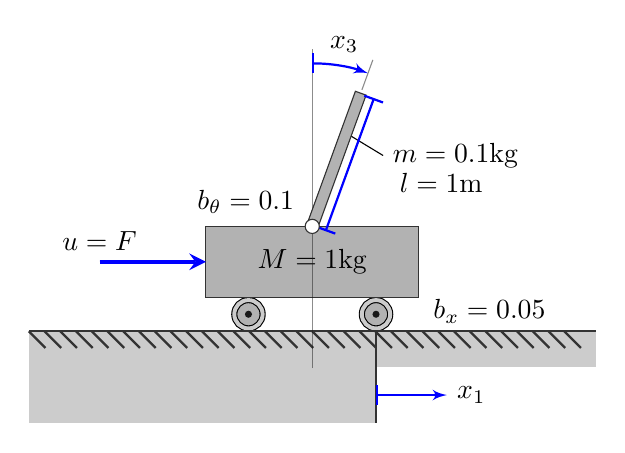
\begin{tikzpicture}[> = latex',%
	scale = 0.9]
	\tikzset{%
		interface/.style={
			% The border decoration is a path replacing decorator. 
			% For the interface style we want to draw the original path.
			% The postaction option is therefore used to ensure that the
			% border decoration is drawn *after* the original path.
			postaction={draw, decorate, decoration={border, angle=-45,
					amplitude=0.3cm, segment length=2mm}}},
		helparrow/.style={>=latex', blue, thick},
		% helparrow/.style={>=latex', draw=blue, fill=blue, very thick},
		helpline/.style={thin, black!90, opacity=0.5},
		force/.style={>=stealth, draw=blue, fill=blue, ultra thick},
	}
	\def\ground{%
		\fill [black!20] (0, 0) rectangle (49mm, -13mm);
		\fill [black!20] (49mm, 0) rectangle (80mm, -5mm);
		\draw [thick, black!80, interface] (0, 0) -- (80mm, 0);
		\draw [thick, black!80] (49mm, 0) -- +(0, -13mm);
		\draw [|->, helparrow] (49mm, -9mm) -- ++(10mm, 0) node [right] {\color{black} $x_1$ };
	}
	
	\def\cart{
		\filldraw [%thick,%
		draw = black!80,%
		fill = black!40,%
		top color = black!30,%
		bottom color = black!30,%
		% pattern=horizontal lines gray,%
		] (0,0) rectangle (30mm, 10mm);
		\node at (15mm, 5mm) {$M=1$kg};
		\draw[->, force] (-15mm, 5mm) node [above] {$u=\ensuremath{\vv{F}}$} -- (0, 5mm);
		\node at (40mm, -2mm) {$b_x = 0.05$};
	}
	
	\def\pendulum{%
		\filldraw [%thick,%
		draw = black!80,%
		% fill = black!25,%
		left color=black!30,%
		bottom color=black!30,%
		% pattern=horizontal lines gray,%
		] (-0.8mm, 0) rectangle (0.8mm, 20mm);
		\draw [|-|, helparrow] (2mm, 0mm) -- ++(0mm, 20mm);
		\node at (15mm, 12mm) {$l=1$m};
		\node at (-10mm, 0mm) {$b_\theta=0.1$}; 
	}
	
	\def\joint{%
		\filldraw [%thick,%
		draw = black!80,%
		fill = white,%
		% pattern=horizontal lines gray,%
		] (0, 0) circle (1mm);
	}
	
	\def\wheel{%
%		\fill [thin,%
%		fill = black!70,%	path fading = south
%	] (0, 0) circle (1.75mm);
%		\begin{scope}
%			\clip (0, 0) circle (1.75mm);
%			\fill [fill=black!30,] (0, -1mm) circle (2mm);
%		\end{scope}
		\fill [fill=black!30,] (0, 0mm) circle (2mm);
		\fill [fill=black!90] (0, 0) circle (0.5mm);
		\draw [thin,%
		double = black!20,%
		double distance = 0.5mm] (0, 0) circle (2mm);
	}

	\begin{scope}
		\wheel
	\end{scope}
	\begin{scope}[xshift=18mm]
		\wheel
	\end{scope}
	\begin{scope}[xshift=-31mm, yshift=-2.4mm]
		\ground
	\end{scope}
	\begin{scope}[shift = {(-6mm, 2.4mm)}]
		\cart
	\end{scope}
	\begin{scope}[shift = {(9mm, 12.4mm)}]
		\draw [helpline] (0, -20mm) -- (0, 25mm);
		\draw [helpline] (70:20.5mm) -- (70:25mm);
		\draw [|->, helparrow] (0, 23mm) 
		arc [radius=23mm, start angle=90, delta angle=-20] ;
		\node at (80:26mm) {$x_3$};
%		\draw [|->, helparrow] (0, -9mm) 
%		arc [radius=9mm, start angle=-90, delta angle=195] ;
%		\node [above right] at (50:8.5mm) {$\theta$};
		\draw [thin] (70:14mm) -- (10mm, 10mm) 
		node [right] {$m=0.1$kg};
	\end{scope}
	\begin{scope}[shift = {(9mm, 12.4mm)}, rotate=-20]
		\pendulum
	\end{scope}
	\begin{scope}[shift = {(9mm, 12.4mm)}]
		\joint
	\end{scope}
\end{tikzpicture}


%\begin{tikzpicture}[> = latex',%
%	scale = 1,%
%	text = blue]
%	\begin{scope}
%		\wheel
%	\end{scope}
%	\begin{scope}[xshift=18mm]
%		\wheel
%	\end{scope}
%	\begin{scope}[xshift=-31mm, yshift=-2.4mm]
%		\ground
%	\end{scope}
%	\begin{scope}[shift = {(-6mm, 2.4mm)}]
%		\cart
%	\end{scope}
%	\begin{scope}[shift = {(9mm, 12.4mm)}]
%		\draw [helpline] (0, -20mm) -- (0, 25mm);
%		\draw [helpline] (110:20.5mm) -- (110:25mm);
%		\draw [|->, helparrow] (0, 23mm) 
%		arc [radius=23mm, start angle=90, delta angle=20] ;
%		\node at (97:25mm) {$\theta'$};
%		\draw [|->, helparrow] (0, -9mm) 
%		arc [radius=9mm, start angle=-90, delta angle=195] ;
%		\node [above right] at (50:8.5mm) {$\theta$};
%		\draw [thin] (110:14mm) -- (-10mm, 10mm) 
%		node [left] {$m$, $I$};
%	\end{scope}
%	\begin{scope}[shift = {(9mm, 12.4mm)}, rotate=20]
%		\pendulum
%	\end{scope}
%	\begin{scope}[shift = {(9mm, 12.4mm)}]
%		\joint
%	\end{scope}
%\end{tikzpicture}
	\caption{Illustration of the inverted pendulum.}\label{fig:invpen}
\end{figure}

Consider the system linearized at $x_3=x_4=0$, and we sample the continuous-time linear system periodically with sampling interval $T_s=0.02$ seconds. 
The system equation is:
\begin{align*}
x(k+1)=\begin{bmatrix}
1  &   2.0\cdot 10^{-2}  &  -2.0\cdot 10^{-4}  &  1.9\cdot 10^{-5}\\
0  &   1.0\cdot 10^{0}   & -2.0\cdot 10^{-2}  &   1.8\cdot 10^{-3}\\
0  &   1.0\cdot 10^{-5} &   1.0\cdot 10^{0} &   2.0\cdot 10^{-2}\\
0  &   1.0\cdot 10^{-3}&  2.1\cdot 10^{-1}  &  9.8\cdot 10^{-1}
\end{bmatrix}x(k)+\begin{bmatrix}
2.0\cdot 10^{-4}\\
2.0\cdot 10^{-2}\\
-2.0\cdot 10^{-4}\\
-2.0\cdot 10^{-2}
\end{bmatrix}
u(k)+w(k).
\end{align*}
\begin{align*}
y(k)=
\begin{bmatrix}
1& 0 &0 &0\\
1& 0 &0 &0\\
1& 0 &0 &0\\
0& 0 &1 &0
\end{bmatrix}x(k)+v(k)+a(k).
\end{align*}
The system dynamic matrix can be written as the following Jordan canonical form by an invertible linear transformation:
$$
\begin{bmatrix}
1.057 & 0 &  0 & 0\\
0  & 1 & 0 &  0\\
0  & 0 & 0.999 & 0  \\
0  & 0 & 0 &  0.925 
\end{bmatrix},
$$
and we consider the system after transformation. System matrix $A$ have four Jordan blocks with size $1\times1$ and the upper left two blocks have unstable eigenvalues. Therefore, the set of unstable states and stable states are $\Uc=\{1,2\},\Sc=\{3,4\}.$
The canonical form of $G_i^\Uc$ are 
\begin{align}
H_1^\Uc=H_2^\Uc=H_3^\Uc=\begin{bmatrix}
1 & 0 \\
0  & 1 \\
0  & 0   \\
0  & 0 
\end{bmatrix},\ H_4^\Uc=\begin{bmatrix}
0 & 0 \\
0  & 1 \\
0  & 0   \\
0  & 0 
\end{bmatrix}.
\end{align}
Only the first 3 sensors can observe unstable state 1, i.e., $\Ec_1=\{1,2,3\}$. All the four sensors can observe unstable state 2, i.e., $\Ec_2=\{1,2,3,4\}$.
Therefore, the system is 2-sparse detectable and our proposed estimator secure in the presence of 1 corrupted sensor. 
In the simulation, the noise covariances of the system are $Q=R=T_s^2\times\diag(0.1,0.1,0.01,0.01)$.
The initial state is assumed to be known by the estimator.
The controller of the system is designed as a Linear-Quadratic Regulator (LQR), and the feedback matrix is chosen as $K_{\rm lqr}=\begin{bmatrix}
	-8& -15& -115 &-32
 \end{bmatrix}.
$
%
%
%In the following we perform state transformation on the origin system to better analysis the observability structure.
%There exists a invertible matrix $U$ such that 
%
%In the following, we study the following system where $\bar{C}\triangleq CU$:
%	\begin{align*}
%		\bar{x}(k+1)&=\bar{A} \bar{x}(k)+U^{-1}w(k)+U^{-1}Bu(k), \\
%		y(k)&=\bar{C} \bar{x}(k)+v(k)+a(k).
%	\end{align*}


We first illustrate the performance of estimation on close-loop system where $u(k)=-K_{\rm lqr} x(k)$.
Fig. \ref{fig:close_loop} presents the performance of the estimation of system states in the absence of attack. Our proposed estimation substantially coincides with the Kalman estimation. The numerical difference attributes to large Gaussian noise that occurs occasionally which violates inequality \eqref{eq:kalman_cond} and error in numerical calculation.


\begin{figure}[htpb!]
	\centering
	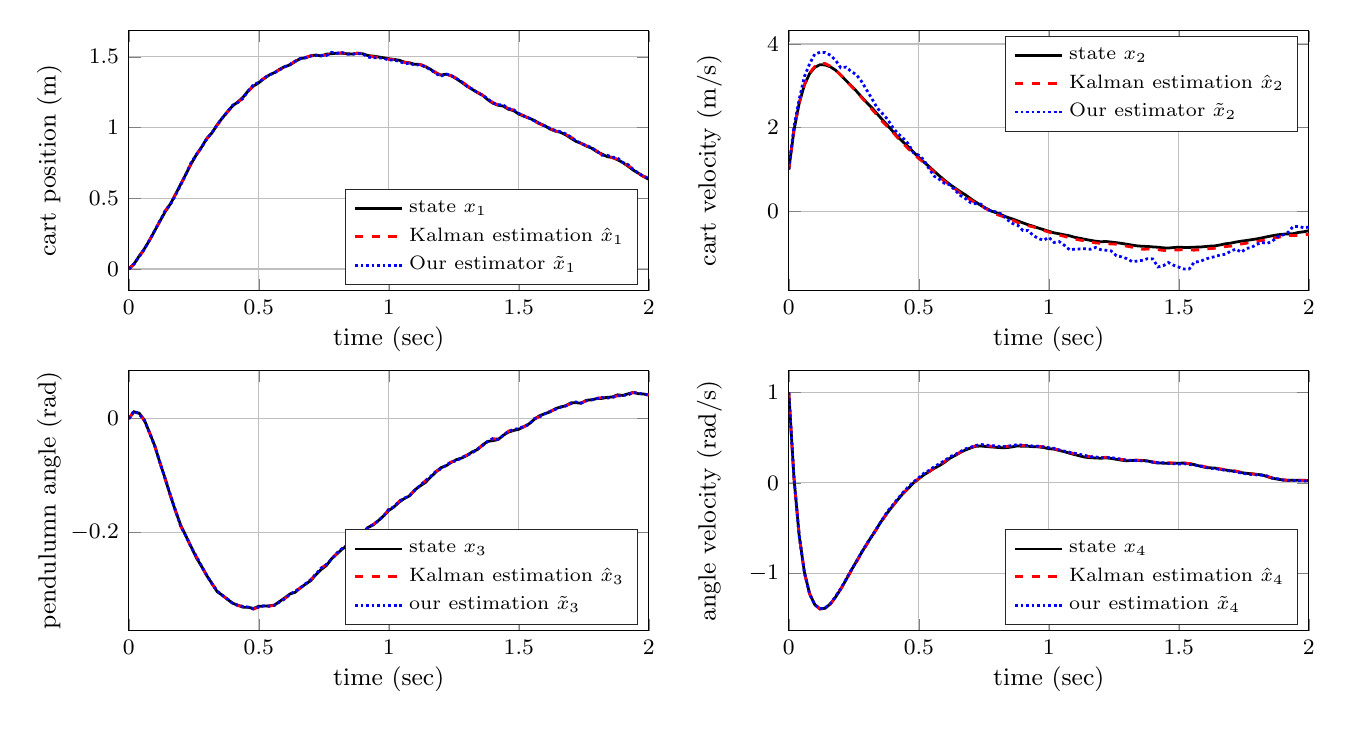
\begin{tikzpicture}
\begin{axis}
[	width=2.6in,
	height=1.3in,
	at={(0in,1.7in)},
	scale only axis,
	xmin=0,
	xmax=2.0,
	xlabel={\small time (sec)},
	ylabel={\small cart position (m)},
	x label style={at={(axis description cs:0.5,-0.1)},anchor=north},
	y label style={at={(axis description cs:-0.11,.5)},anchor=south},
	xticklabel style = {font=\footnotesize},
	yticklabel style = {font=\footnotesize},
	axis background/.style={fill=white},
	xmajorgrids,
	ymajorgrids,
	legend style={at={(0.98,0.02)}, anchor=south east, legend cell align=left, align=left, draw=white!15!black, font=\scriptsize }]
	 \addplot [color={black}, line width=1pt]
	table[row sep={\\}]
	{
 0.0  0.0  \\
0.02  0.03513048308256195  \\
0.04  0.0914419059773598  \\
0.06  0.1427778787943515  \\
0.08  0.20340397252067047  \\
0.1  0.27125016952880654  \\
0.12  0.33866874289613796  \\
0.14  0.40444843392896823  \\
0.16  0.46015949841787734  \\
0.18  0.5289069560917001  \\
0.2  0.6012564469268484  \\
0.22  0.671516604288933  \\
0.24  0.7439326698612437  \\
0.26  0.8082019623524164  \\
0.28  0.8613988630585795  \\
0.3  0.9229014124726718  \\
0.32  0.9627944492478866  \\
0.34  1.0198488236259264  \\
0.36  1.0678031171226763  \\
0.38  1.1139131874770454  \\
0.4  1.1540061381552729  \\
0.42  1.1817601868900285  \\
0.44  1.2153756793882182  \\
0.46  1.2610010644181515  \\
0.48  1.293667654117393  \\
0.5  1.3165928728936251  \\
0.52  1.3456607164297567  \\
0.54  1.3711705993370278  \\
0.56  1.3880813521098108  \\
0.58  1.4119643858187543  \\
0.6  1.4306314658383006  \\
0.62  1.4425883212114448  \\
0.64  1.4662379310448435  \\
0.66  1.4886979846322503  \\
0.68  1.4923086118898035  \\
0.7  1.5069041141339614  \\
0.72  1.5128680594921478  \\
0.74  1.505743231730095  \\
0.76  1.5189247374151202  \\
0.78  1.5218381993746002  \\
0.8  1.5255446307745213  \\
0.82  1.5253720117652096  \\
0.84  1.5217505378866258  \\
0.86  1.519753386225738  \\
0.88  1.5257526690458258  \\
0.9  1.521386537923482  \\
0.92  1.5089559694196168  \\
0.94  1.5049195077352266  \\
0.96  1.4993578292639884  \\
0.98  1.493191880058802  \\
1.0  1.4864024420058506  \\
1.02  1.4818259580594746  \\
1.04  1.475808315831528  \\
1.06  1.462990519709879  \\
1.08  1.4570631794200655  \\
1.1  1.4471759284474504  \\
1.12  1.446272982684707  \\
1.14  1.4313922548235627  \\
1.16  1.4124330091086377  \\
1.18  1.3872010233567227  \\
1.2  1.3711358431710576  \\
1.22  1.3771278026366942  \\
1.24  1.3667791681890535  \\
1.26  1.3445038037339296  \\
1.28  1.3202679649240783  \\
1.3  1.2930882108314934  \\
1.32  1.2708701152599298  \\
1.34  1.248239872310746  \\
1.36  1.2293771367777346  \\
1.38  1.1977995399651467  \\
1.4  1.172303904975972  \\
1.42  1.1579161820351642  \\
1.44  1.1518067463014627  \\
1.46  1.12924061744534  \\
1.48  1.1195894705658813  \\
1.5  1.0955432603592228  \\
1.52  1.0797265742904583  \\
1.54  1.066608150282723  \\
1.56  1.0502266993513543  \\
1.58  1.0281772752372773  \\
1.6  1.0130822665150812  \\
1.62  0.9895403519101377  \\
1.64  0.9750991121836318  \\
1.66  0.9665183092659061  \\
1.68  0.9491107003879848  \\
1.7  0.9250252075044484  \\
1.72  0.9023279997906815  \\
1.74  0.8883577172905913  \\
1.76  0.868997041684394  \\
1.78  0.8542728121099745  \\
1.8  0.8295422463647049  \\
1.82  0.812162366888937  \\
1.84  0.7943357438050268  \\
1.86  0.7883783454959857  \\
1.88  0.7721739750301243  \\
1.9  0.7527806629178648  \\
1.92  0.7271547015768657  \\
1.94  0.699425481543776  \\
1.96  0.6770173029804786  \\
1.98  0.6539652107821747  \\
2.0  0.6339162103868775  \\
	}
	;\addlegendentry{state $x_1$}
	
	\addplot [color={red},dashed, line width=1pt]
	table[row sep={\\}]
	{
 0.0  0.0  \\
0.02  0.03459224381061867  \\
0.04  0.08529450384877155  \\
0.06  0.14037092177605182  \\
0.08  0.20553954051240308  \\
0.1  0.27194944336447746  \\
0.12  0.3421140054880376  \\
0.14  0.41203750940323125  \\
0.16  0.4622193750988459  \\
0.18  0.5275770920396385  \\
0.2  0.5965866800336724  \\
0.22  0.6697110178836443  \\
0.24  0.7482230113686512  \\
0.26  0.8092656626309191  \\
0.28  0.8603169832513828  \\
0.3  0.9190552078813129  \\
0.32  0.9650153184004646  \\
0.34  1.017537438416803  \\
0.36  1.0652639550276204  \\
0.38  1.110203819001036  \\
0.4  1.1547227063481849  \\
0.42  1.1795489385299753  \\
0.44  1.2081962408148317  \\
0.46  1.2550663978277128  \\
0.48  1.29773491819716  \\
0.5  1.3202634853421826  \\
0.52  1.3485493090138312  \\
0.54  1.3730537082664092  \\
0.56  1.3887333644343987  \\
0.58  1.4096399363306875  \\
0.6  1.4291719543335981  \\
0.62  1.4458626407157713  \\
0.64  1.4681322460180737  \\
0.66  1.4857860140746912  \\
0.68  1.4965623645092951  \\
0.7  1.5064593300461164  \\
0.72  1.5105362942780847  \\
0.74  1.5102375963545158  \\
0.76  1.510715778888172  \\
0.78  1.5270954377963672  \\
0.8  1.5246804945886832  \\
0.82  1.5285375327524982  \\
0.84  1.5219032482401056  \\
0.86  1.520849497046739  \\
0.88  1.5251716736489362  \\
0.9  1.524289721395395  \\
0.92  1.505448635516613  \\
0.94  1.4999695126483625  \\
0.96  1.4960501263894108  \\
0.98  1.4934718949769015  \\
1.0  1.4818326310727334  \\
1.02  1.480707330754286  \\
1.04  1.4726414641854848  \\
1.06  1.4602017028591072  \\
1.08  1.4578204430879882  \\
1.1  1.4469453164906172  \\
1.12  1.4458062938261007  \\
1.14  1.4329313953696996  \\
1.16  1.4160364457991061  \\
1.18  1.3897188031328918  \\
1.2  1.3679973969686312  \\
1.22  1.3751905872313022  \\
1.24  1.3655727389377705  \\
1.26  1.3488207107801553  \\
1.28  1.3275020222766156  \\
1.3  1.297676742947427  \\
1.32  1.2702012536827056  \\
1.34  1.2502056805120871  \\
1.36  1.2294028774129964  \\
1.38  1.2047001213441297  \\
1.4  1.1764390180689184  \\
1.42  1.16036795764531  \\
1.44  1.155022054177548  \\
1.46  1.133504665669269  \\
1.48  1.123504538352717  \\
1.5  1.1008427846179605  \\
1.52  1.0822931182727697  \\
1.54  1.0645682653691237  \\
1.56  1.0440920436330998  \\
1.58  1.0263246901040088  \\
1.6  1.0083507822846796  \\
1.62  0.9920679329287192  \\
1.64  0.976622670428748  \\
1.66  0.965578948875552  \\
1.68  0.9523055143949263  \\
1.7  0.9325703449798766  \\
1.72  0.907991669348745  \\
1.74  0.8873053457649742  \\
1.76  0.8709858398455673  \\
1.78  0.8557650883330062  \\
1.8  0.8339912648523344  \\
1.82  0.8066085662950583  \\
1.84  0.7985872884191355  \\
1.86  0.7867861486514177  \\
1.88  0.7761000737630973  \\
1.9  0.7490347746578546  \\
1.92  0.732851128940592  \\
1.94  0.703824889092848  \\
1.96  0.6780744090491957  \\
1.98  0.6534946070984852  \\
2.0  0.6408473560775105  \\
	}
	;\addlegendentry{{ Kalman estimation $\hat{x}_1$}}
    \addplot[densely dotted, color={blue}, line width=1pt]
        table[row sep={\\}]
        {
    0.0  1.4977176879243853e-7  \\
   0.02  0.035853490924953726  \\
   0.04  0.08728505927307653  \\
   0.06  0.1402910759956027  \\
   0.08  0.20552535131997382  \\
   0.1  0.2714941202711113  \\
   0.12  0.34142780537522516  \\
   0.14  0.41073226781224864  \\
   0.16  0.4544716293659916  \\
   0.18  0.523689684730239  \\
   0.2  0.59571397823773  \\
   0.22  0.6714956021666036  \\
   0.24  0.7527759703720808  \\
   0.26  0.8099977345031584  \\
   0.28  0.8585085304808415  \\
   0.3  0.9201763916641157  \\
   0.32  0.9634570022906116  \\
   0.34  1.0194972876060886  \\
   0.36  1.0682564396376053  \\
   0.38  1.1136126645917057  \\
   0.4  1.158888312085378  \\
   0.42  1.178120027939495  \\
   0.44  1.2073589678987888  \\
   0.46  1.26043900840599  \\
   0.48  1.3032407211239458  \\
   0.5  1.3196645821997441  \\
   0.52  1.3483934150336057  \\
   0.54  1.372515904226193  \\
   0.56  1.3860504677892873  \\
   0.58  1.4085218217648232  \\
   0.6  1.4289739159288626  \\
   0.62  1.4463131599581733  \\
   0.64  1.469263537104824  \\
   0.66  1.4859403959732742  \\
   0.68  1.4946012652267906  \\
   0.7  1.5054772861342394  \\
   0.72  1.508985002964067  \\
   0.74  1.5090595106705802  \\
   0.76  1.5100025471877747  \\
   0.78  1.5316171969246877  \\
   0.8  1.5250681057932682  \\
   0.82  1.5299726074216564  \\
   0.84  1.5187812082208154  \\
   0.86  1.5179027994705732  \\
   0.88  1.5229965752350674  \\
   0.9  1.5207666604060461  \\
   0.92  1.4969719778684472  \\
   0.94  1.494447987716439  \\
   0.96  1.4922607037710425  \\
   0.98  1.4901753577011345  \\
   1.0  1.4764885137636086  \\
   1.02  1.4772125891950725  \\
   1.04  1.4682067816915458  \\
   1.06  1.4530770280512573  \\
   1.08  1.453827951153766  \\
   1.1  1.441609631566825  \\
   1.12  1.4440558602407247  \\
   1.14  1.4286081399465453  \\
   1.16  1.4105638904580435  \\
   1.18  1.3825173171614653  \\
   1.2  1.3621514478144654  \\
   1.22  1.3791831050328722  \\
   1.24  1.367315529077668  \\
   1.26  1.3476206221565943  \\
   1.28  1.3245829684293324  \\
   1.3  1.2922967385204185  \\
   1.32  1.2732201761350186  \\
   1.34  1.2489868087093448  \\
   1.36  1.2293982024530576  \\
   1.38  1.2043499531068822  \\
   1.4  1.1741781296701639  \\
   1.42  1.1611707415378525  \\
   1.44  1.1598795804587332  \\
   1.46  1.134112124666843  \\
   1.48  1.126562052033941  \\
   1.5  1.099894827177205  \\
   1.52  1.0815913921937006  \\
   1.54  1.065892705016733  \\
   1.56  1.0463019361723187  \\
   1.58  1.0286992509406694  \\
   1.6  1.0106514622486629  \\
   1.62  0.9951516048130251  \\
   1.64  0.9799038849666539  \\
   1.66  0.9700959717111278  \\
   1.68  0.9557138008265439  \\
   1.7  0.9335952475399413  \\
   1.72  0.9071514346753368  \\
   1.74  0.8872958166261384  \\
   1.76  0.8730466086745535  \\
   1.78  0.8581694338561564  \\
   1.8  0.8343792855852288  \\
   1.82  0.8049652888616172  \\
   1.84  0.8040552514089182  \\
   1.86  0.7915587983875398  \\
   1.88  0.7844327028764996  \\
   1.9  0.7527655411430587  \\
   1.92  0.7383308407971062  \\
   1.94  0.704573733557403  \\
   1.96  0.6786187118658552  \\
   1.98  0.6540139211205167  \\
   2.0  0.6447964303367395  \\
        }
        ;\addlegendentry{{ Our estimator $\tilde{x}_1$}}
        
\end{axis}

\begin{axis}
[	width=2.6in,
height=1.3in,
at={(3.3in,1.7in)},
scale only axis,
xmin=0,
xmax=2.0,
xlabel={\small time (sec)},
ylabel={\small cart velocity (m/s)},
x label style={at={(axis description cs:0.5,-0.1)},anchor=north},
y label style={at={(axis description cs:-0.11,.5)},anchor=south},
xticklabel style = {font=\footnotesize},
yticklabel style = {font=\footnotesize},
axis background/.style={fill=white},
xmajorgrids,
ymajorgrids,
legend style={at={(0.98,0.98)}, anchor=north east, legend cell align=left, align=left, draw=white!15!black, font=\scriptsize}]
\addplot [color={black}, line width=1pt]
table[row sep={\\}]
{
	   0.0  1.0  \\
	0.02  1.9334581216414537  \\
	0.04  2.5813598448326145  \\
	0.06  3.0186330460084227  \\
	0.08  3.291179056338291  \\
	0.1  3.4420274187060738  \\
	0.12  3.505817976791329  \\
	0.14  3.499891224562881  \\
	0.16  3.4541824320967547  \\
	0.18  3.3738782752424057  \\
	0.2  3.2556305585295  \\
	0.22  3.1274116627100383  \\
	0.24  3.0026901645012507  \\
	0.26  2.874184622899233  \\
	0.28  2.7341536239027664  \\
	0.3  2.599092680673387  \\
	0.32  2.474338381258081  \\
	0.34  2.3295685255856236  \\
	0.36  2.189281790708088  \\
	0.38  2.050610403342911  \\
	0.4  1.9112709141422126  \\
	0.42  1.7724690892688961  \\
	0.44  1.6556812877910012  \\
	0.46  1.5363521105995848  \\
	0.48  1.4150465701315613  \\
	0.5  1.2871220460497423  \\
	0.52  1.173898127416659  \\
	0.54  1.0669077212594953  \\
	0.56  0.9531860356888151  \\
	0.58  0.842766455685593  \\
	0.6  0.7368526011631864  \\
	0.62  0.6386885141858373  \\
	0.64  0.5522982987768248  \\
	0.66  0.4673970287861549  \\
	0.68  0.388441452040231  \\
	0.7  0.298284094139456  \\
	0.72  0.21521130663157695  \\
	0.74  0.13527244786941045  \\
	0.76  0.06775133614445589  \\
	0.78  0.0018217977639210792  \\
	0.8  -0.041362523286636844  \\
	0.82  -0.09381421061386852  \\
	0.84  -0.14407979447997937  \\
	0.86  -0.18381986538803088  \\
	0.88  -0.23073184780733264  \\
	0.9  -0.2768618767232452  \\
	0.92  -0.3221050406495692  \\
	0.94  -0.3590270204895619  \\
	0.96  -0.4031121866973199  \\
	0.98  -0.440255543871223  \\
	1.0  -0.4794506820094533  \\
	1.02  -0.5164186629794366  \\
	1.04  -0.5394774520685265  \\
	1.06  -0.5648929581179745  \\
	1.08  -0.5880335616899929  \\
	1.1  -0.6240583811993707  \\
	1.12  -0.6475946969073231  \\
	1.14  -0.6726280234431121  \\
	1.16  -0.6962591244562204  \\
	1.18  -0.716170488653756  \\
	1.2  -0.7303439029290554  \\
	1.22  -0.723794234408197  \\
	1.24  -0.7372309153786233  \\
	1.26  -0.752398594469176  \\
	1.28  -0.7689826700011977  \\
	1.3  -0.7887195432951313  \\
	1.32  -0.8098867523071835  \\
	1.34  -0.8283635747294913  \\
	1.36  -0.8385252691562912  \\
	1.38  -0.8425053705736679  \\
	1.4  -0.8530276369062237  \\
	1.42  -0.8611447646232143  \\
	1.44  -0.8755583704269705  \\
	1.46  -0.880004440081546  \\
	1.48  -0.8689920459015796  \\
	1.5  -0.8595727805783289  \\
	1.52  -0.8664261794787972  \\
	1.54  -0.8666080222698963  \\
	1.56  -0.858959104753468  \\
	1.58  -0.8582703425085555  \\
	1.6  -0.8457675726072812  \\
	1.62  -0.8351131490600251  \\
	1.64  -0.8277078898807627  \\
	1.66  -0.8050674915577795  \\
	1.68  -0.778258009757186  \\
	1.7  -0.7625851887730555  \\
	1.72  -0.7367569207114357  \\
	1.74  -0.7162352969327319  \\
	1.76  -0.7002081907735124  \\
	1.78  -0.6805254062776667  \\
	1.8  -0.6612425270314914  \\
	1.82  -0.6373058472130902  \\
	1.84  -0.610364894464108  \\
	1.86  -0.5860224964571155  \\
	1.88  -0.5644176597159203  \\
	1.9  -0.5497525352056346  \\
	1.92  -0.5436161322897733  \\
	1.94  -0.5370160070749582  \\
	1.96  -0.5071817392955478  \\
	1.98  -0.4917082598298192  \\
	2.0  -0.4666136152945374  \\
}
;\addlegendentry{state $x_2$}

\addplot [color={red},dashed, line width=1pt]
table[row sep={\\}]
{
 0.0  1.0  \\
0.02  1.947272359389003  \\
0.04  2.594445635915076  \\
0.06  3.0275370892357465  \\
0.08  3.3064047984742215  \\
0.1  3.462393973240511  \\
0.12  3.5337552017316733  \\
0.14  3.5316267806993924  \\
0.16  3.470940986138043  \\
0.18  3.376126341013576  \\
0.2  3.2566259086770186  \\
0.22  3.120943910267192  \\
0.24  2.994733431504582  \\
0.26  2.8615793698700442  \\
0.28  2.7190991877286375  \\
0.3  2.5871944838338887  \\
0.32  2.4357929803750835  \\
0.34  2.297296006782219  \\
0.36  2.146799297184839  \\
0.38  2.018946597493442  \\
0.4  1.889014652512622  \\
0.42  1.7487315098372516  \\
0.44  1.624824088563198  \\
0.46  1.4897200993389361  \\
0.48  1.3810698328950473  \\
0.5  1.2596631340531221  \\
0.52  1.1634939872696184  \\
0.54  1.0480627830829743  \\
0.56  0.9308302914400389  \\
0.58  0.8123785236046864  \\
0.6  0.7148330468660997  \\
0.62  0.6265455625597441  \\
0.64  0.5331502434450455  \\
0.66  0.43205816222084126  \\
0.68  0.3483303867886185  \\
0.7  0.2658684830316831  \\
0.72  0.1986892314490598  \\
0.74  0.12940453547456832  \\
0.76  0.057090111696830426  \\
0.78  -0.022323517297730522  \\
0.8  -0.07855954509213436  \\
0.82  -0.1196590633380139  \\
0.84  -0.16482030375100798  \\
0.86  -0.21334051972282897  \\
0.88  -0.26764929753246003  \\
0.9  -0.3085925202001949  \\
0.92  -0.34729926263317723  \\
0.94  -0.37389141047737684  \\
0.96  -0.4186172810225557  \\
0.98  -0.4604016560194364  \\
1.0  -0.49774276614583723  \\
1.02  -0.5415613192539162  \\
1.04  -0.5732363853566289  \\
1.06  -0.6009216622984934  \\
1.08  -0.6361620967828028  \\
1.1  -0.6662684185318611  \\
1.12  -0.6910234803017076  \\
1.14  -0.7091492500091724  \\
1.16  -0.7326867589147015  \\
1.18  -0.7583372537059867  \\
1.2  -0.7678701553484749  \\
1.22  -0.775291203531666  \\
1.24  -0.7826361711427366  \\
1.26  -0.7891963194264477  \\
1.28  -0.8137146002990012  \\
1.3  -0.8366439913742113  \\
1.32  -0.8590459273741499  \\
1.34  -0.8777808029848111  \\
1.36  -0.9088564448755428  \\
1.38  -0.9052762284220978  \\
1.4  -0.9103017076540781  \\
1.42  -0.9217620312291152  \\
1.44  -0.9360252496793352  \\
1.46  -0.9439912115605257  \\
1.48  -0.9257262139038105  \\
1.5  -0.9248197561970852  \\
1.52  -0.9208562202142578  \\
1.54  -0.9280099457265346  \\
1.56  -0.9307959004598831  \\
1.58  -0.9226143412383395  \\
1.6  -0.9040398340982976  \\
1.62  -0.8937141414658287  \\
1.64  -0.8857428368393998  \\
1.66  -0.866305242987084  \\
1.68  -0.8441684653507048  \\
1.7  -0.8353086527257382  \\
1.72  -0.8050702996023907  \\
1.74  -0.7845056910274278  \\
1.76  -0.7650158652157595  \\
1.78  -0.7376887920799782  \\
1.8  -0.723084297668014  \\
1.82  -0.6992720095891855  \\
1.84  -0.677183773374071  \\
1.86  -0.6432509338919762  \\
1.88  -0.6298213424768249  \\
1.9  -0.5970448968271864  \\
1.92  -0.5853791165420197  \\
1.94  -0.5788058486799379  \\
1.96  -0.5782348686628517  \\
1.98  -0.5671551428159235  \\
2.0  -0.551581774220117  \\
}
;\addlegendentry{{ Kalman estimation $\hat{x}_2$}}
\addplot[densely dotted, color={blue}, line width=1pt]
table[row sep={\\}]
{
 0.0  0.9999999921251895  \\
0.02  2.0212895754401674  \\
0.04  2.6756392857258184  \\
0.06  3.221956367906082  \\
0.08  3.524459948415112  \\
0.1  3.7597636021985625  \\
0.12  3.801231238982991  \\
0.14  3.799637195005116  \\
0.16  3.7327542013131265  \\
0.18  3.6111856404678333  \\
0.2  3.430534859904597  \\
0.22  3.4485602236994395  \\
0.24  3.3444533813093464  \\
0.26  3.2665237848301816  \\
0.28  3.1042853013055063  \\
0.3  2.8967222342877976  \\
0.32  2.6907577163441476  \\
0.34  2.470727224887547  \\
0.36  2.33691826338607  \\
0.38  2.200387456547136  \\
0.4  2.0020638149880137  \\
0.42  1.8570627601031489  \\
0.44  1.747672024063133  \\
0.46  1.611155911903882  \\
0.48  1.3963895051585353  \\
0.5  1.3408628051804476  \\
0.52  1.2247463441132191  \\
0.54  1.010654566111314  \\
0.56  0.8344555369735892  \\
0.58  0.7584015792726887  \\
0.6  0.6632429865275014  \\
0.62  0.6293946727583775  \\
0.64  0.4985199207634023  \\
0.66  0.37640264139319624  \\
0.68  0.3011719349763173  \\
0.7  0.20268409454240105  \\
0.72  0.17876010231844372  \\
0.74  0.16927357874176333  \\
0.76  0.04338529646943603  \\
0.78  0.002109695471169712  \\
0.8  -0.01550391409818583  \\
0.82  -0.0747172626157792  \\
0.84  -0.20114517757971595  \\
0.86  -0.29154879522700883  \\
0.88  -0.3342275025568856  \\
0.9  -0.46051997938139294  \\
0.92  -0.4592290442747301  \\
0.94  -0.5784388075160722  \\
0.96  -0.6525450159385416  \\
0.98  -0.695320153788558  \\
1.0  -0.6240888206867699  \\
1.02  -0.7463217729066517  \\
1.04  -0.726975101951553  \\
1.06  -0.8138167061427473  \\
1.08  -0.9235454222917523  \\
1.1  -0.9069665295941886  \\
1.12  -0.9006953548896325  \\
1.14  -0.8974900363513572  \\
1.16  -0.9094084162227737  \\
1.18  -0.8664730452439139  \\
1.2  -0.9202891565839497  \\
1.22  -0.9328018978926498  \\
1.24  -0.9508543283041255  \\
1.26  -1.0646735023491174  \\
1.28  -1.0912248536913043  \\
1.3  -1.1331402926510883  \\
1.32  -1.203643871217519  \\
1.34  -1.1922974521406433  \\
1.36  -1.1738986207825004  \\
1.38  -1.1350262927165347  \\
1.4  -1.1414974965228946  \\
1.42  -1.331862785682863  \\
1.44  -1.3060932513394654  \\
1.46  -1.2275118049260128  \\
1.48  -1.2914442441963048  \\
1.5  -1.3372485123883435  \\
1.52  -1.3820301256548315  \\
1.54  -1.3821000075562804  \\
1.56  -1.2137564286546132  \\
1.58  -1.207557673691415  \\
1.6  -1.1516263695735407  \\
1.62  -1.1129690587856955  \\
1.64  -1.0850379975163027  \\
1.66  -1.045131304276628  \\
1.68  -1.0292639388423739  \\
1.7  -0.9523308895320762  \\
1.72  -0.905240368310937  \\
1.74  -0.9804802293648478  \\
1.76  -0.8910154468115234  \\
1.78  -0.8648663571953334  \\
1.8  -0.7900802207875451  \\
1.82  -0.7486111807501488  \\
1.84  -0.769284934870073  \\
1.86  -0.7162288714699678  \\
1.88  -0.6108822217212676  \\
1.9  -0.5685703272065101  \\
1.92  -0.5058158657185248  \\
1.94  -0.3633224811381064  \\
1.96  -0.3634413413786554  \\
1.98  -0.393417228111549  \\
2.0  -0.38005238786555934  \\
}
;\addlegendentry{{ Our estimator $\tilde{x}_2$}}

\end{axis}

  	\begin{axis}
	[	width=2.6in,
	height=1.3in,
	at={(0in,0in)},
	scale only axis,
	xmin=0,
	xmax=2.0,
%	ymin=-4,
%	ymax=2,
	xlabel={\small time (sec)},
	ylabel={\small pendulumn angle (rad)},
	x label style={at={(axis description cs:0.5,-0.1)},anchor=north},
	y label style={at={(axis description cs:-0.11,.5)},anchor=south},
	xticklabel style = {font=\footnotesize},
	yticklabel style = {font=\footnotesize},
	axis background/.style={fill=white},
	xmajorgrids,
	ymajorgrids,
	legend style={at={(0.98,0.02)}, anchor=south east, legend cell align=left, align=left, draw=white!15!black, font=\scriptsize}]
	\addplot [color={black}, line width=1pt]
	table[row sep={\\}]
	{
	0.0  0.0  \\
	0.02  0.012291107212995766  \\
	0.04  0.009755897813268646  \\
	0.06  -0.0021158879924274895  \\
	0.08  -0.0247027096213208  \\
	0.1  -0.04772264515761605  \\
	0.12  -0.07760140828511264  \\
	0.14  -0.10540107095412833  \\
	0.16  -0.13522977096567482  \\
	0.18  -0.1625910350853779  \\
	0.2  -0.18762454463647446  \\
	0.22  -0.20648175697703935  \\
	0.24  -0.2253718219740834  \\
	0.26  -0.2446837803311821  \\
	0.28  -0.2598043838864768  \\
	0.3  -0.27605718927768963  \\
	0.32  -0.29005282855504183  \\
	0.34  -0.3042957897577329  \\
	0.36  -0.31049253276580696  \\
	0.38  -0.3180784063475375  \\
	0.4  -0.3246605763946356  \\
	0.42  -0.3281158539923102  \\
	0.44  -0.3316915860721911  \\
	0.46  -0.331794893198938  \\
	0.48  -0.33385309324954493  \\
	0.5  -0.3298748808806763  \\
	0.52  -0.32962332567317526  \\
	0.54  -0.32935520726148154  \\
	0.56  -0.3278096251813507  \\
	0.58  -0.32156766834611766  \\
	0.6  -0.31514570998488606  \\
	0.62  -0.3082586040066044  \\
	0.64  -0.30531014110059096  \\
	0.66  -0.2974893495725164  \\
	0.68  -0.2909982672931626  \\
	0.7  -0.28476233098070064  \\
	0.72  -0.2741691441756372  \\
	0.74  -0.26514320719682183  \\
	0.76  -0.25834616090694207  \\
	0.78  -0.2463839079177759  \\
	0.8  -0.23800597979646262  \\
	0.82  -0.2297059475101298  \\
	0.84  -0.22320522465660433  \\
	0.86  -0.21473029965939316  \\
	0.88  -0.2078124562987345  \\
	0.9  -0.20054438831726454  \\
	0.92  -0.191255406523477  \\
	0.94  -0.18694955107462255  \\
	0.96  -0.17918753992578848  \\
	0.98  -0.1709426605116633  \\
	1.0  -0.1613919061973941  \\
	1.02  -0.15508350580114946  \\
	1.04  -0.14671305238418206  \\
	1.06  -0.1403268225084615  \\
	1.08  -0.13574733780874354  \\
	1.1  -0.12525543807074938  \\
	1.12  -0.11830891826074295  \\
	1.14  -0.11245711089028443  \\
	1.16  -0.10307527657908676  \\
	1.18  -0.09427290168258842  \\
	1.2  -0.08624311487904997  \\
	1.22  -0.08281286220423259  \\
	1.24  -0.07694032858147544  \\
	1.26  -0.07202084211561871  \\
	1.28  -0.06915277041228256  \\
	1.3  -0.06482535296933563  \\
	1.32  -0.0585286985478911  \\
	1.34  -0.0544178260128904  \\
	1.36  -0.04631622791370163  \\
	1.38  -0.039964573256803776  \\
	1.4  -0.03847838945946058  \\
	1.42  -0.03672894464324935  \\
	1.44  -0.029174405131490357  \\
	1.46  -0.02359523707621013  \\
	1.48  -0.020619335181098767  \\
	1.5  -0.018521871195534556  \\
	1.52  -0.014018688360862593  \\
	1.54  -0.00887576952604927  \\
	1.56  -0.0009549249582036146  \\
	1.58  0.005369382629282453  \\
	1.6  0.008923746760306408  \\
	1.62  0.012014243079846536  \\
	1.64  0.017493783523120362  \\
	1.66  0.02063669578966442  \\
	1.68  0.022777301401473927  \\
	1.7  0.02792901936340122  \\
	1.72  0.0283241284450547  \\
	1.74  0.027254422457167155  \\
	1.76  0.032589984297573586  \\
	1.78  0.03338585890332495  \\
	1.8  0.035379761925010626  \\
	1.82  0.035895798593158466  \\
	1.84  0.0377253385620041  \\
	1.86  0.0383662690861781  \\
	1.88  0.04210618064021919  \\
	1.9  0.041098254254943775  \\
	1.92  0.04377317376047081  \\
	1.94  0.04648024578966923  \\
	1.96  0.04418348421073788  \\
	1.98  0.043582409046281606  \\
	2.0  0.04168602319521932  \\
	}
	;\addlegendentry{state $x_3$}
	\addplot [color={red},dashed, line width=1pt]
	table[row sep={\\}]
	{
	 0.0  0.0  \\
	0.02  0.013426852424592635  \\
	0.04  0.00843301396563128  \\
	0.06  -0.0032719716704107363  \\
	0.08  -0.02481652590182395  \\
	0.1  -0.0481640290053725  \\
	0.12  -0.0773260791503746  \\
	0.14  -0.1058336782375687  \\
	0.16  -0.13437583604937386  \\
	0.18  -0.16212078795551588  \\
	0.2  -0.18936680035330689  \\
	0.22  -0.20682682816877246  \\
	0.24  -0.22624739266974847  \\
	0.26  -0.24255240711015966  \\
	0.28  -0.25938100915865997  \\
	0.3  -0.27582223696323216  \\
	0.32  -0.29017509895378113  \\
	0.34  -0.30312551898597867  \\
	0.36  -0.3108404318615062  \\
	0.38  -0.3175096992310906  \\
	0.4  -0.32477739971223507  \\
	0.42  -0.32872249274395  \\
	0.44  -0.33018903736083494  \\
	0.46  -0.33157421359120864  \\
	0.48  -0.3347682789953573  \\
	0.5  -0.3312864817244998  \\
	0.52  -0.3291627726596654  \\
	0.54  -0.3297666385420164  \\
	0.56  -0.3282382129572867  \\
	0.58  -0.32238470924044726  \\
	0.6  -0.31672569552127106  \\
	0.62  -0.3085504873331749  \\
	0.64  -0.30358250382869933  \\
	0.66  -0.29773744780767014  \\
	0.68  -0.29016275624136845  \\
	0.7  -0.28324232741969124  \\
	0.72  -0.2732071282504288  \\
	0.74  -0.26281750327886394  \\
	0.76  -0.2564093284426296  \\
	0.78  -0.24688582045630497  \\
	0.8  -0.23677699922420448  \\
	0.82  -0.22836242552414882  \\
	0.84  -0.22245410156213347  \\
	0.86  -0.21530514692305724  \\
	0.88  -0.20682501773654127  \\
	0.9  -0.20132726494700445  \\
	0.92  -0.19133634121209478  \\
	0.94  -0.1860795054846685  \\
	0.96  -0.17923265589551396  \\
	0.98  -0.17123226535783656  \\
	1.0  -0.15947304935805745  \\
	1.02  -0.1548388172456593  \\
	1.04  -0.14520227739515446  \\
	1.06  -0.13967063081873776  \\
	1.08  -0.13497786067807926  \\
	1.1  -0.12577412934247395  \\
	1.12  -0.1175337223799782  \\
	1.14  -0.10944005723868216  \\
	1.16  -0.10203913130146214  \\
	1.18  -0.09308715477437135  \\
	1.2  -0.08794796965792803  \\
	1.22  -0.08185246218716763  \\
	1.24  -0.07600601687938979  \\
	1.26  -0.07381608821932717  \\
	1.28  -0.06864813536384877  \\
	1.3  -0.06395460212857695  \\
	1.32  -0.0602261386722721  \\
	1.34  -0.05382440640690687  \\
	1.36  -0.04712363867652214  \\
	1.38  -0.04002379686199878  \\
	1.4  -0.03497080113403436  \\
	1.42  -0.036111152278679635  \\
	1.44  -0.029620305752766234  \\
	1.46  -0.021773164700165097  \\
	1.48  -0.019294421438656367  \\
	1.5  -0.016478689404025585  \\
	1.52  -0.013809213558272245  \\
	1.54  -0.009727493539955652  \\
	1.56  0.00010697132410502795  \\
	1.58  0.003604031000592948  \\
	1.6  0.008688099632814618  \\
	1.62  0.012944729342028295  \\
	1.64  0.016592536427066158  \\
	1.66  0.020277043802924465  \\
	1.68  0.02257961530726481  \\
	1.7  0.026839618915516762  \\
	1.72  0.029657998521030172  \\
	1.74  0.027805946665924633  \\
	1.76  0.03180101991605573  \\
	1.78  0.033066821117509665  \\
	1.8  0.035885805832444086  \\
	1.82  0.03732698332095191  \\
	1.84  0.03641690235064062  \\
	1.86  0.037608010230084615  \\
	1.88  0.04046959465662314  \\
	1.9  0.04083718635296667  \\
	1.92  0.042140952368440815  \\
	1.94  0.046116066215212054  \\
	1.96  0.04496044143824164  \\
	1.98  0.042846010266078184  \\
	2.0  0.04215378271487344  \\
	}
	;\addlegendentry{{ Kalman estimation $\hat{x}_3$}}
	\addplot[densely dotted, color={blue}, line width=1pt]
	table[row sep={\\}]
	{
	  0.0  3.1433028608416316e-11  \\
	0.02  0.01344847021277637  \\
	0.04  0.008456418975972609  \\
	0.06  -0.003219574862069982  \\
	0.08  -0.02475805266926738  \\
	0.1  -0.048084890121452485  \\
	0.12  -0.07725623252920924  \\
	0.14  -0.10576373127871824  \\
	0.16  -0.1343109389730368  \\
	0.18  -0.16206335020175422  \\
	0.2  -0.1893260123921801  \\
	0.22  -0.20674474366208784  \\
	0.24  -0.22615857471885029  \\
	0.26  -0.24244984963046978  \\
	0.28  -0.2592849482472964  \\
	0.3  -0.27574565258076134  \\
	0.32  -0.29011468126158285  \\
	0.34  -0.3030849181196164  \\
	0.36  -0.31079415153767914  \\
	0.38  -0.31746475450630307  \\
	0.4  -0.32475059932585915  \\
	0.42  -0.3286979958750598  \\
	0.44  -0.3301566350657236  \\
	0.46  -0.3315454057362295  \\
	0.48  -0.33476539666787736  \\
	0.5  -0.33126459223915605  \\
	0.52  -0.3291446171754128  \\
	0.54  -0.32977682333152664  \\
	0.56  -0.3282644310786887  \\
	0.58  -0.32239992793632893  \\
	0.6  -0.3167376923759136  \\
	0.62  -0.3085475743064995  \\
	0.64  -0.30359190886766  \\
	0.66  -0.29775518117534255  \\
	0.68  -0.2901767867638945  \\
	0.7  -0.2832625348316812  \\
	0.72  -0.2732108435292309  \\
	0.74  -0.26280663960011597  \\
	0.76  -0.2564159355046562  \\
	0.78  -0.24688204211903556  \\
	0.8  -0.23676259103857464  \\
	0.82  -0.22835230844078408  \\
	0.84  -0.22246562892342184  \\
	0.86  -0.21532691142003657  \\
	0.88  -0.2068442861454246  \\
	0.9  -0.20136824017592664  \\
	0.92  -0.19136447635253848  \\
	0.94  -0.1861313446823315  \\
	0.96  -0.17929319817646316  \\
	0.98  -0.1712913427238095  \\
	1.0  -0.15950353420499566  \\
	1.02  -0.15489450584642925  \\
	1.04  -0.14524273291189224  \\
	1.06  -0.13972735953720475  \\
	1.08  -0.13505461765357452  \\
	1.1  -0.12583533518582937  \\
	1.12  -0.11758925372920472  \\
	1.14  -0.10948757785994269  \\
	1.16  -0.10208415445996129  \\
	1.18  -0.09311647703886469  \\
	1.2  -0.08798920559108425  \\
	1.22  -0.08189633429516247  \\
	1.24  -0.07605045258975703  \\
	1.26  -0.07388888332934941  \\
	1.28  -0.06872358366327118  \\
	1.3  -0.06403512588379763  \\
	1.32  -0.06031880849722568  \\
	1.34  -0.05390843262445146  \\
	1.36  -0.047195908591125865  \\
	1.38  -0.040084203489465196  \\
	1.4  -0.03503401262632256  \\
	1.42  -0.036220695262529044  \\
	1.44  -0.029718190884273927  \\
	1.46  -0.021848754400959458  \\
	1.48  -0.01939066854636683  \\
	1.5  -0.0165878607075766  \\
	1.52  -0.01393033314624452  \\
	1.54  -0.00984796249146883  \\
	1.56  3.2439964015529796e-5  \\
	1.58  0.003528261632672118  \\
	1.6  0.00862371058623918  \\
	1.62  0.012887565405679638  \\
	1.64  0.016540197860918194  \\
	1.66  0.020229548981544734  \\
	1.68  0.022530692928118046  \\
	1.7  0.026807904118887373  \\
	1.72  0.029632732673344667  \\
	1.74  0.027753413760428246  \\
	1.76  0.03176884410287142  \\
	1.78  0.03303614023475411  \\
	1.8  0.035869861526218454  \\
	1.82  0.037316297307355514  \\
	1.84  0.036393231851024214  \\
	1.86  0.037593384983039296  \\
	1.88  0.04047659192861037  \\
	1.9  0.04084873814081459  \\
	1.92  0.04216512575394451  \\
	1.94  0.04617317081672683  \\
	1.96  0.04501482701743717  \\
	1.98  0.04288794903185354  \\
	2.0  0.04219731519953074  \\
	}
;\addlegendentry{{our estimation $\tilde{x}_3$}}


\end{axis}

\begin{axis}
[	width=2.6in,
height=1.3in,
at={(3.3in,0in)},
scale only axis,
xmin=0,
xmax=2.0,
%ymin=-4,
%ymax=2,
xlabel={\small time (sec)},
ylabel={\small angle velocity (rad/s)},
x label style={at={(axis description cs:0.5,-0.1)},anchor=north},
y label style={at={(axis description cs:-0.11,.5)},anchor=south},
xticklabel style = {font=\footnotesize},
yticklabel style = {font=\footnotesize},
axis background/.style={fill=white},
xmajorgrids,
ymajorgrids,
legend style={at={(0.98,0.02)}, anchor=south east, legend cell align=left, align=left, draw=white!15!black, font=\scriptsize}]
\addplot [color={black}, line width=1pt]
table[row sep={\\}]
{
  0.0  1.0  \\
0.02  0.05313305390126177  \\
0.04  -0.5807597079886778  \\
0.06  -0.9849649892184913  \\
0.08  -1.2236616544745775  \\
0.1  -1.3448708265564777  \\
0.12  -1.3911973425235322  \\
0.14  -1.3847017109780744  \\
0.16  -1.3360588370385862  \\
0.18  -1.2612956960549269  \\
0.2  -1.1712121233640451  \\
0.22  -1.071999578445813  \\
0.24  -0.9674797110228057  \\
0.26  -0.8680549183886634  \\
0.28  -0.7699884280336178  \\
0.3  -0.6746842796248621  \\
0.32  -0.586875654761506  \\
0.34  -0.4959299174041296  \\
0.36  -0.40597661697079446  \\
0.38  -0.32771095994654365  \\
0.4  -0.253961547290701  \\
0.42  -0.18263871652089975  \\
0.44  -0.11573407741218594  \\
0.46  -0.05911515161120641  \\
0.48  0.0009801138197992887  \\
0.5  0.04463813200237973  \\
0.52  0.09038368590143643  \\
0.54  0.12381466371390598  \\
0.56  0.16193471899976158  \\
0.58  0.19217803962499197  \\
0.6  0.2284585486584002  \\
0.62  0.27315223526991256  \\
0.64  0.3029744279918313  \\
0.66  0.3360381761463694  \\
0.68  0.36405311581028843  \\
0.7  0.3862145241118462  \\
0.72  0.4052381391063923  \\
0.74  0.40659407112164414  \\
0.76  0.4016463115722345  \\
0.78  0.39680426743202124  \\
0.8  0.3921338510569967  \\
0.82  0.3884591608505884  \\
0.84  0.3897778445333768  \\
0.86  0.3978434385510643  \\
0.88  0.40888248291393214  \\
0.9  0.40349125898703586  \\
0.92  0.4043181979298124  \\
0.94  0.4001713487291486  \\
0.96  0.397537790317619  \\
0.98  0.3906342747298136  \\
1.0  0.377882856254513  \\
1.02  0.3727858562415341  \\
1.04  0.3579748382263377  \\
1.06  0.34457979003538486  \\
1.08  0.3274365776280705  \\
1.1  0.31223393396172927  \\
1.12  0.2972605478138003  \\
1.14  0.28374482940224277  \\
1.16  0.27808313315371463  \\
1.18  0.2752540519763583  \\
1.2  0.27226461109496636  \\
1.22  0.27696110635321103  \\
1.24  0.26990768271144283  \\
1.26  0.26054532527838425  \\
1.28  0.2504740216554849  \\
1.3  0.24312004848395827  \\
1.32  0.24828658502523776  \\
1.34  0.2471687742404289  \\
1.36  0.2483512476352048  \\
1.38  0.2421106054905815  \\
1.4  0.2281155213543221  \\
1.42  0.2192043397969218  \\
1.44  0.21813440821530206  \\
1.46  0.215847499113375  \\
1.48  0.21810640903792972  \\
1.5  0.21793606071633792  \\
1.52  0.21839791991053367  \\
1.54  0.21094224607272868  \\
1.56  0.20175648284456538  \\
1.58  0.18577552098976302  \\
1.6  0.17234252915874954  \\
1.62  0.1667589628096436  \\
1.64  0.16336600936391402  \\
1.66  0.15026901018454916  \\
1.68  0.1427360828668787  \\
1.7  0.13367410170858618  \\
1.72  0.12734499958354706  \\
1.74  0.11405351681196844  \\
1.76  0.10587244286568445  \\
1.78  0.10156266429081387  \\
1.8  0.0936679758808678  \\
1.82  0.08822122445956102  \\
1.84  0.07018133601995245  \\
1.86  0.05094537909202273  \\
1.88  0.04130087142500513  \\
1.9  0.032313361980953  \\
1.92  0.02866897811479254  \\
1.94  0.030018199155337016  \\
1.96  0.029179914657290675  \\
1.98  0.029178093401201616  \\
2.0  0.02640041419686011  \\
}
;\addlegendentry{state $x_4$}
\addplot [color={red},dashed, line width=1pt]
table[row sep={\\}]
{
0.0  1.0  \\
0.02  0.05196229099537668  \\
0.04  -0.5824313535988286  \\
0.06  -0.9891377715191895  \\
0.08  -1.225040556372666  \\
0.1  -1.3474376677420603  \\
0.12  -1.3927650448471267  \\
0.14  -1.3853875418228592  \\
0.16  -1.3385535189542455  \\
0.18  -1.2616908106226903  \\
0.2  -1.1733481356619362  \\
0.22  -1.0733971982561636  \\
0.24  -0.9709048883726853  \\
0.26  -0.8734509930998627  \\
0.28  -0.7737477786715035  \\
0.3  -0.6814462079764667  \\
0.32  -0.5930068323706987  \\
0.34  -0.5011111690344067  \\
0.36  -0.4117486708366517  \\
0.38  -0.32787217975647187  \\
0.4  -0.25500615240975977  \\
0.42  -0.18223637558459482  \\
0.44  -0.1136859116043202  \\
0.46  -0.05435490540626656  \\
0.48  0.001052155333388885  \\
0.5  0.047862836014496535  \\
0.52  0.09307612385402939  \\
0.54  0.12661541422593295  \\
0.56  0.16673898540858903  \\
0.58  0.20040364092746082  \\
0.6  0.2378257684031066  \\
0.62  0.28092995786664526  \\
0.64  0.30722850104675375  \\
0.66  0.33988761950874746  \\
0.68  0.3717014698259486  \\
0.7  0.39114473419457757  \\
0.72  0.41074056965705785  \\
0.74  0.4157082365437478  \\
0.76  0.4107206907578836  \\
0.78  0.40479797621004415  \\
0.8  0.4002479612239634  \\
0.82  0.39670525295180864  \\
0.84  0.402980720989716  \\
0.86  0.40966660580558506  \\
0.88  0.41939855229643713  \\
0.9  0.4136774603389678  \\
0.92  0.41337706589827294  \\
0.94  0.4076360923733703  \\
0.96  0.40419133912255345  \\
0.98  0.39738214224816115  \\
1.0  0.38613613596819135  \\
1.02  0.37863833492291044  \\
1.04  0.3613171630485197  \\
1.06  0.34817084130208276  \\
1.08  0.3337665386001098  \\
1.1  0.322513876054837  \\
1.12  0.30951293238535926  \\
1.14  0.29822140789925367  \\
1.16  0.2887209415996951  \\
1.18  0.2855447198327156  \\
1.2  0.2792019100681843  \\
1.22  0.28259480121327957  \\
1.24  0.27674766540821855  \\
1.26  0.2679337895584435  \\
1.28  0.25957147095312993  \\
1.3  0.2512852868921737  \\
1.32  0.25335034594023265  \\
1.34  0.2517049563980485  \\
1.36  0.24854241554762116  \\
1.38  0.2437570887642059  \\
1.4  0.232081337423728  \\
1.42  0.2246763936573522  \\
1.44  0.22593853025256636  \\
1.46  0.22180580292165525  \\
1.48  0.2201777881736648  \\
1.5  0.21772174841998373  \\
1.52  0.22039359761167476  \\
1.54  0.21451665272588324  \\
1.56  0.20671496543671092  \\
1.58  0.19237907013470915  \\
1.6  0.17849341727408496  \\
1.62  0.1693669711801831  \\
1.64  0.1654694365161853  \\
1.66  0.15476608715270937  \\
1.68  0.14644491458503275  \\
1.7  0.1380087312073818  \\
1.72  0.12999696162763208  \\
1.74  0.11642996712779241  \\
1.76  0.10651977489569771  \\
1.78  0.09914327961373791  \\
1.8  0.09326070775598083  \\
1.82  0.08760116773835838  \\
1.84  0.07441328030636729  \\
1.86  0.0534154762075595  \\
1.88  0.04537417203289343  \\
1.9  0.03311477519912949  \\
1.92  0.029386264188961075  \\
1.94  0.031449452742925314  \\
1.96  0.028203792066178256  \\
1.98  0.026902194874244584  \\
2.0  0.023968301890876745  \\
}
;\addlegendentry{{ Kalman estimation $\hat{x}_4$}}
\addplot[densely dotted, color={blue}, line width=1pt]
table[row sep={\\}]
{
   0.0  0.9999999995931783  \\
0.02  0.053256438469400355  \\
0.04  -0.5810558367590097  \\
0.06  -0.9888797959421549  \\
0.08  -1.223881505907738  \\
0.1  -1.3453082018539748  \\
0.12  -1.3891303460776288  \\
0.14  -1.379673068887711  \\
0.16  -1.3337025957314825  \\
0.18  -1.253342000372752  \\
0.2  -1.165825320019194  \\
0.22  -1.0647406851480974  \\
0.24  -0.962864368017885  \\
0.26  -0.8669013996514804  \\
0.28  -0.7648147896002787  \\
0.3  -0.6716102653407486  \\
0.32  -0.5837308230993299  \\
0.34  -0.49443467840184724  \\
0.36  -0.40249690841846597  \\
0.38  -0.3131891235819798  \\
0.4  -0.2447579085019484  \\
0.42  -0.17249116699733316  \\
0.44  -0.1030719454933759  \\
0.46  -0.04285668755265462  \\
0.48  0.0114903655938736  \\
0.5  0.058227653678667265  \\
0.52  0.10717166963032067  \\
0.54  0.1384072775498972  \\
0.56  0.18001465974339406  \\
0.58  0.2133703433896741  \\
0.6  0.2465157229825645  \\
0.62  0.28971937610144716  \\
0.64  0.3129481166649311  \\
0.66  0.3450497044394353  \\
0.68  0.37686103961345435  \\
0.7  0.3936878232730471  \\
0.72  0.4150532260957958  \\
0.74  0.4233531164511129  \\
0.76  0.4171875013483728  \\
0.78  0.41134854117958397  \\
0.8  0.4070401399420528  \\
0.82  0.39934970941532405  \\
0.84  0.4045038112026713  \\
0.86  0.41167154833883346  \\
0.88  0.42410157171426555  \\
0.9  0.4146297227803898  \\
0.92  0.4139524638829347  \\
0.94  0.40661075476522757  \\
0.96  0.4036843661018631  \\
0.98  0.39802668389530804  \\
1.0  0.38824401885059434  \\
1.02  0.38239487320383886  \\
1.04  0.3633355958402282  \\
1.06  0.35065780164947047  \\
1.08  0.33821632861934037  \\
1.1  0.3269686985664032  \\
1.12  0.31461866216272727  \\
1.14  0.30171518500382105  \\
1.16  0.28963383826350086  \\
1.18  0.2873988907364934  \\
1.2  0.27659891830676514  \\
1.22  0.2815743584939091  \\
1.24  0.2796811226753734  \\
1.26  0.2697498149899335  \\
1.28  0.26134056909419723  \\
1.3  0.24959006217362836  \\
1.32  0.2504781981325628  \\
1.34  0.24593217671946835  \\
1.36  0.2426440319644277  \\
1.38  0.24079990072853516  \\
1.4  0.22929989748022161  \\
1.42  0.22198397772499973  \\
1.44  0.22259088456441103  \\
1.46  0.21489558149696208  \\
1.48  0.21275644734565288  \\
1.5  0.20717683010408106  \\
1.52  0.21169927725858503  \\
1.54  0.20412663702544515  \\
1.56  0.19746398862601647  \\
1.58  0.1869741075430982  \\
1.6  0.173740420161395  \\
1.62  0.1604900026037437  \\
1.64  0.15756553133036336  \\
1.66  0.1481590395148509  \\
1.68  0.13805716699049428  \\
1.7  0.13040946307195095  \\
1.72  0.12253183558288747  \\
1.74  0.10883203724797469  \\
1.76  0.09907761486652333  \\
1.78  0.09264569886581496  \\
1.8  0.08851705283528442  \\
1.82  0.08454416975622558  \\
1.84  0.07506523004933284  \\
1.86  0.053058346159098005  \\
1.88  0.04567485530664184  \\
1.9  0.031371123950315244  \\
1.92  0.02706214943933832  \\
1.94  0.02810347265390892  \\
1.96  0.024086348522412558  \\
1.98  0.02104640638710214  \\
2.0  0.021127296064900145  \\
}
;\addlegendentry{{our estimation $\tilde{x}_4$}}


\end{axis}

\end{tikzpicture}





	\caption{Estimation of states in the absence of attack. The initial state is $x(0)=[0,\ 1,\ 0,\ 1]{'}$. } \label{fig:close_loop}
\end{figure}

Fig \ref{fig:attack_signal} shows the injected attack signal on sensor 3 and the corresponding observations from sensor 3.
Fig. \ref{fig:close_loop_attack} demonstrates the estimation with the attack shown in Fig. \ref{fig:attack_signal}.
The attack $a_3(k)$ is a time-independent random value uniformly distributed on interval $(-1,1)$. As shown in the figure, Kalman estimation (denoted as red dashed line) has larger estimation error than our proposed estimation under the attack.

\begin{figure}[ht]
	\centering
	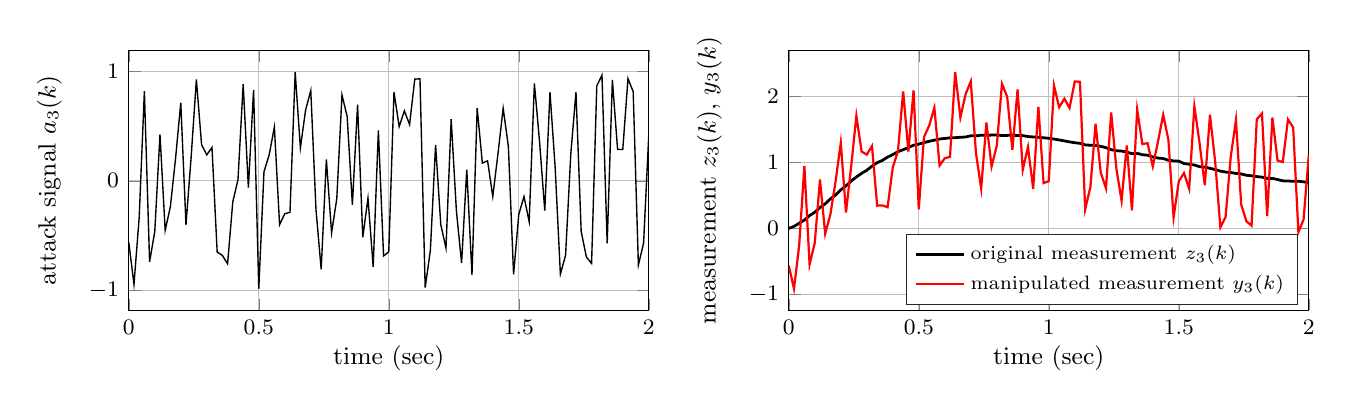
\begin{tikzpicture}
\begin{axis}
[	width=2.6in,
	height=1.3in,
	at={(0in,1.7in)},
	scale only axis,
	xmin=0,
	xmax=2.0,
	xlabel={\small time (sec)},
	ylabel={\small attack signal $a_3(k)$},
	x label style={at={(axis description cs:0.5,-0.1)},anchor=north},
	y label style={at={(axis description cs:-0.11,.5)},anchor=south},
	xticklabel style = {font=\footnotesize},
	yticklabel style = {font=\footnotesize},
	axis background/.style={fill=white},
	xmajorgrids,
	ymajorgrids,
	legend style={at={(0.98,0.02)}, anchor=south east, legend cell align=left, align=left, draw=white!15!black, font=\scriptsize}]
	 \addplot [color={black}, line width=0.5pt]
	table[row sep={\\}]
	{
0.0  -0.5625685225246384  \\
0.02  -0.946157670457147  \\
0.04  -0.3364104982135254  \\
0.06  0.8202072091057051  \\
0.08  -0.7416794304773182  \\
0.1  -0.4636695887925457  \\
0.12  0.4247375003814464  \\
0.14  -0.4529398288478932  \\
0.16  -0.23609426388419186  \\
0.18  0.20607156940463156  \\
0.2  0.7146776978338217  \\
0.22  -0.4031811551171538  \\
0.24  0.2206252826036046  \\
0.26  0.9264480578446211  \\
0.28  0.33016511715381247  \\
0.3  0.23718509653538966  \\
0.32  0.3053190945443012  \\
0.34  -0.6512496890635018  \\
0.36  -0.6822150171560071  \\
0.38  -0.7591862879712541  \\
0.4  -0.19280907417578508  \\
0.42  0.010038743472394973  \\
0.44  0.8827731819816345  \\
0.46  -0.06232326649906916  \\
0.48  0.8319345169225183  \\
0.5  -0.9872827034407057  \\
0.52  0.08252119515841416  \\
0.54  0.23761861917437788  \\
0.56  0.4911335147891096  \\
0.58  -0.40195620239799457  \\
0.6  -0.3007915416907321  \\
0.62  -0.2880389885558321  \\
0.64  0.9936238737504954  \\
0.66  0.301057855330896  \\
0.68  0.6458920116460922  \\
0.7  0.825439900787106  \\
0.72  -0.2620778554704919  \\
0.74  -0.8099631243406966  \\
0.76  0.19437015142373726  \\
0.78  -0.4755865591670845  \\
0.8  -0.16394509461018458  \\
0.82  0.7845865898376772  \\
0.84  0.5867174223091793  \\
0.86  -0.2193032349255386  \\
0.88  0.6958595916418464  \\
0.9  -0.5164339756771317  \\
0.92  -0.15836646301569557  \\
0.94  -0.7857843469695074  \\
0.96  0.46132582292170277  \\
0.98  -0.6869516269713491  \\
1.0  -0.6493852750653204  \\
1.02  0.8112005067738504  \\
1.04  0.49552013490097657  \\
1.06  0.6395260827687634  \\
1.08  0.5144317327991712  \\
1.1  0.9294456667948578  \\
1.12  0.9324288820292381  \\
1.14  -0.9769366346964161  \\
1.16  -0.6351510189600362  \\
1.18  0.32726158838108965  \\
1.2  -0.40098100760181365  \\
1.22  -0.6150064270922488  \\
1.24  0.5641016529988976  \\
1.26  -0.27231215515339535  \\
1.28  -0.752554332947537  \\
1.3  0.10187427646239922  \\
1.32  -0.8600011844841662  \\
1.34  0.6642700257000524  \\
1.36  0.16170120198315496  \\
1.38  0.1826664933681159  \\
1.4  -0.14334483866806247  \\
1.42  0.2486222622627241  \\
1.44  0.6622426969022284  \\
1.46  0.3136861979015393  \\
1.48  -0.8557620863445856  \\
1.5  -0.3070342555493415  \\
1.52  -0.14416760270375484  \\
1.54  -0.37368830515195883  \\
1.56  0.8911874844829586  \\
1.58  0.35518376316127453  \\
1.6  -0.27339031973850947  \\
1.62  0.8105521223144891  \\
1.64  0.11784059265095037  \\
1.66  -0.8529040350736259  \\
1.68  -0.6806944273502968  \\
1.7  0.24363510423789958  \\
1.72  0.8110402429453711  \\
1.74  -0.4624898957872765  \\
1.76  -0.6967699885218077  \\
1.78  -0.7555009870069109  \\
1.8  0.8677999951918474  \\
1.82  0.9651388566369782  \\
1.84  -0.572692343156155  \\
1.86  0.9214722802132305  \\
1.88  0.28714732919033314  \\
1.9  0.28600006541082534  \\
1.92  0.9336419255406856  \\
1.94  0.8153373412752746  \\
1.96  -0.771121795555112  \\
1.98  -0.5703813934558002  \\
2.0  0.4202296393480983  \\
	};
	

\end{axis}

\begin{axis}
[	width=2.6in,
height=1.3in,
at={(3.3in,1.7in)},
scale only axis,
xmin=0,
xmax=2.0,
xlabel={\small time (sec)},
ylabel={\small measurement $z_3(k)$, $y_3(k)$},
x label style={at={(axis description cs:0.5,-0.1)},anchor=north},
y label style={at={(axis description cs:-0.11,.5)},anchor=south},
xticklabel style = {font=\footnotesize},
yticklabel style = {font=\footnotesize},
axis background/.style={fill=white},
xmajorgrids,
ymajorgrids,
legend style={at={(0.98,0.02)}, anchor=south east, legend cell align=left, align=left, draw=white!15!black, font=\scriptsize}]
\addplot [color={black}, line width=1pt]
table[row sep={\\}]
{
	0.0  0.0005061476188890966  \\
	0.02  0.031676588671764164  \\
	0.04  0.07839140216717005  \\
	0.06  0.12705814413038907  \\
	0.08  0.19480431491342415  \\
	0.1  0.24606443660984756  \\
	0.12  0.3172084112413346  \\
	0.14  0.3736461521457517  \\
	0.16  0.44787503073264906  \\
	0.18  0.5069223027691104  \\
	0.2  0.5852364000596318  \\
	0.22  0.6450996948371481  \\
	0.24  0.719598187094292  \\
	0.26  0.7802246068858262  \\
	0.28  0.8352976511484314  \\
	0.3  0.8819249843701404  \\
	0.32  0.9438334235786126  \\
	0.34  0.9968137130862087  \\
	0.36  1.0315121996566714  \\
	0.38  1.081352724577131  \\
	0.4  1.1186852002911756  \\
	0.42  1.1641077812910212  \\
	0.44  1.1939659134273448  \\
	0.46  1.2272556361330376  \\
	0.48  1.261665715825486  \\
	0.5  1.2786078316998268  \\
	0.52  1.3011683448134117  \\
	0.54  1.321384821506629  \\
	0.56  1.338382036174266  \\
	0.58  1.355281400342649  \\
	0.6  1.3648091021791213  \\
	0.62  1.3732953101805965  \\
	0.64  1.3762112690389299  \\
	0.66  1.382112031788601  \\
	0.68  1.3860206445448202  \\
	0.7  1.4048404930230238  \\
	0.72  1.4039269899470739  \\
	0.74  1.4137690804441447  \\
	0.76  1.4113935296580151  \\
	0.78  1.415466288691426  \\
	0.8  1.4173504637099132  \\
	0.82  1.408216099780143  \\
	0.84  1.410853101252453  \\
	0.86  1.4122366732375526  \\
	0.88  1.4099148151176653  \\
	0.9  1.4068220459084428  \\
	0.92  1.3932771447410874  \\
	0.94  1.3869197810882306  \\
	0.96  1.3816719911696593  \\
	0.98  1.3746540193141819  \\
	1.0  1.3668281178807369  \\
	1.02  1.3552820898141782  \\
	1.04  1.3412950137254243  \\
	1.06  1.327392873379449  \\
	1.08  1.312190740537211  \\
	1.1  1.2995220178320626  \\
	1.12  1.290181413888831  \\
	1.14  1.2667219743156652  \\
	1.16  1.2612298991666215  \\
	1.18  1.2589715517767963  \\
	1.2  1.2447068247074753  \\
	1.22  1.2246558090903343  \\
	1.24  1.1947392767545253  \\
	1.26  1.178691587432372  \\
	1.28  1.1725210952749316  \\
	1.3  1.1574143114167688  \\
	1.32  1.1333554895621063  \\
	1.34  1.1379319746939296  \\
	1.36  1.1176217433173101  \\
	1.38  1.1102593716696092  \\
	1.4  1.0836873054208704  \\
	1.42  1.067036714947158  \\
	1.44  1.0605533729454986  \\
	1.46  1.0344992068703907  \\
	1.48  1.0243303238705184  \\
	1.5  1.020077500634661  \\
	1.52  0.9839768264319667  \\
	1.54  0.973260433229496  \\
	1.56  0.9617053886606732  \\
	1.58  0.936138032340902  \\
	1.6  0.9293793225658402  \\
	1.62  0.9117291638631297  \\
	1.64  0.8920858206651604  \\
	1.66  0.8695958676647998  \\
	1.68  0.8548008571060354  \\
	1.7  0.8475448183415518  \\
	1.72  0.8342039556123342  \\
	1.74  0.8264765990017806  \\
	1.76  0.806244182872368  \\
	1.78  0.798659029368042  \\
	1.8  0.7863949401958488  \\
	1.82  0.7781995154823723  \\
	1.84  0.7591860534071165  \\
	1.86  0.7588840404102928  \\
	1.88  0.7418834336133863  \\
	1.9  0.7215463501855689  \\
	1.92  0.7193921889269146  \\
	1.94  0.714570339094586  \\
	1.96  0.7160728188691623  \\
	1.98  0.7071802256678278  \\
	2.0  0.6911892058577479  \\
}
;\addlegendentry{original measurement $z_3(k)$}

\addplot [color={red}, line width=0.8pt]
table[row sep={\\}]
{
   0.0  -0.5620623749057493  \\
0.02  -0.9144810817853829  \\
0.04  -0.25801909604635537  \\
0.06  0.9472653532360942  \\
0.08  -0.546875115563894  \\
0.1  -0.21760515218269816  \\
0.12  0.741945911622781  \\
0.14  -0.07929367670214149  \\
0.16  0.2117807668484572  \\
0.18  0.712993872173742  \\
0.2  1.2999140978934536  \\
0.22  0.24191853971999433  \\
0.24  0.9402234696978966  \\
0.26  1.7066726647304473  \\
0.28  1.1654627683022438  \\
0.3  1.11911008090553  \\
0.32  1.2491525181229137  \\
0.34  0.3455640240227069  \\
0.36  0.3492971825006643  \\
0.38  0.32216643660587696  \\
0.4  0.9258761261153905  \\
0.42  1.1741465247634162  \\
0.44  2.0767390954089793  \\
0.46  1.1649323696339684  \\
0.48  2.0936002327480043  \\
0.5  0.29132512825912116  \\
0.52  1.3836895399718259  \\
0.54  1.559003440681007  \\
0.56  1.8295155509633756  \\
0.58  0.9533251979446544  \\
0.6  1.0640175604883892  \\
0.62  1.0852563216247644  \\
0.64  2.3698351427894253  \\
0.66  1.683169887119497  \\
0.68  2.0319126561909124  \\
0.7  2.23028039381013  \\
0.72  1.141849134476582  \\
0.74  0.6038059561034481  \\
0.76  1.6057636810817524  \\
0.78  0.9398797295243415  \\
0.8  1.2534053690997287  \\
0.82  2.19280268961782  \\
0.84  1.9975705235616323  \\
0.86  1.192933438312014  \\
0.88  2.1057744067595117  \\
0.9  0.8903880702313112  \\
0.92  1.2349106817253919  \\
0.94  0.6011354341187232  \\
0.96  1.842997814091362  \\
0.98  0.6877023923428327  \\
1.0  0.7174428428154165  \\
1.02  2.1664825965880286  \\
1.04  1.8368151486264008  \\
1.06  1.9669189561482123  \\
1.08  1.8266224733363823  \\
1.1  2.2289676846269204  \\
1.12  2.222610295918069  \\
1.14  0.2897853396192491  \\
1.16  0.6260788802065853  \\
1.18  1.586233140157886  \\
1.2  0.8437258171056616  \\
1.22  0.6096493819980855  \\
1.24  1.7588409297534229  \\
1.26  0.9063794322789767  \\
1.28  0.4199667623273946  \\
1.3  1.259288587879168  \\
1.32  0.2733543050779401  \\
1.34  1.802202000393982  \\
1.36  1.279322945300465  \\
1.38  1.292925865037725  \\
1.4  0.940342466752808  \\
1.42  1.3156589772098821  \\
1.44  1.722796069847727  \\
1.46  1.34818540477193  \\
1.48  0.16856823752593275  \\
1.5  0.7130432450853195  \\
1.52  0.8398092237282119  \\
1.54  0.5995721280775371  \\
1.56  1.8528928731436318  \\
1.58  1.2913217955021765  \\
1.6  0.6559890028273307  \\
1.62  1.7222812861776189  \\
1.64  1.0099264133161108  \\
1.66  0.016691832591173905  \\
1.68  0.17410642975573853  \\
1.7  1.0911799225794514  \\
1.72  1.6452441985577053  \\
1.74  0.3639867032145041  \\
1.76  0.10947419435056027  \\
1.78  0.04315804236113108  \\
1.8  1.6541949353876961  \\
1.82  1.7433383721193505  \\
1.84  0.1864937102509615  \\
1.86  1.6803563206235232  \\
1.88  1.0290307628037194  \\
1.9  1.0075464155963942  \\
1.92  1.6530341144676002  \\
1.94  1.5299076803698606  \\
1.96  -0.05504897668594966  \\
1.98  0.1367988322120276  \\
2.0  1.1114188452058462  \\
}
;\addlegendentry{{manipulated measurement $y_3(k)$}}


\end{axis}

%  	\begin{axis}
%	[	width=2.6in,
%	height=1.3in,
%	at={(0in,0in)},
%	scale only axis,
%	xmin=0,
%	xmax=2.0,
%%	ymin=-4,
%%	ymax=2,
%	xlabel={\small time (sec)},
%	ylabel={\small $x_3$ pendulumn angle},
%	x label style={at={(axis description cs:0.5,-0.1)},anchor=north},
%	y label style={at={(axis description cs:-0.11,.5)},anchor=south},
%	xticklabel style = {font=\footnotesize},
%	yticklabel style = {font=\footnotesize},
%	axis background/.style={fill=white},
%	xmajorgrids,
%	ymajorgrids,
%	legend style={at={(0.98,0.02)}, anchor=south east, legend cell align=left, align=left, draw=white!15!black, font=\scriptsize}]
%	\addplot [color={black}, line width=1pt]
%	table[row sep={\\}]
%	{
%0.0  0.0  \\
%0.02  0.00772853593415913  \\
%0.04  0.004801671416923327  \\
%0.06  -0.012528997431996048  \\
%0.08  -0.034478619332425936  \\
%0.1  -0.06220231524500317  \\
%0.12  -0.08812635048651297  \\
%0.14  -0.11408845091735348  \\
%0.16  -0.14488997218330013  \\
%0.18  -0.16947348245078697  \\
%0.2  -0.19501471373927462  \\
%0.22  -0.2166030568036244  \\
%0.24  -0.23694887645664164  \\
%0.26  -0.2534179553657174  \\
%0.28  -0.2659048131170473  \\
%0.3  -0.2814074322954603  \\
%0.32  -0.2947651384686937  \\
%0.34  -0.30280625979339526  \\
%0.36  -0.3110461733895194  \\
%0.38  -0.322599925444607  \\
%0.4  -0.3266601375700984  \\
%0.42  -0.32832183302190043  \\
%0.44  -0.33079378651792585  \\
%0.46  -0.33139999061403563  \\
%0.48  -0.33190912976035625  \\
%0.5  -0.32830514918189446  \\
%0.52  -0.3265624628054656  \\
%0.54  -0.3231032971609128  \\
%0.56  -0.31943423376946206  \\
%0.58  -0.31567219360956844  \\
%0.6  -0.3139459878003922  \\
%0.62  -0.30858429971742735  \\
%0.64  -0.302866065490615  \\
%0.66  -0.2975240107704187  \\
%0.68  -0.29156813130488785  \\
%0.7  -0.28705864201984305  \\
%0.72  -0.2800613967051828  \\
%0.74  -0.2721345042496352  \\
%0.76  -0.2675647476463787  \\
%0.78  -0.26004373544306775  \\
%0.8  -0.24895562242482422  \\
%0.82  -0.24469615255703123  \\
%0.84  -0.23679296240647962  \\
%0.86  -0.22526462977535064  \\
%0.88  -0.21530137387528134  \\
%0.9  -0.2019610820610649  \\
%0.92  -0.19283115640996426  \\
%0.94  -0.18404650174938508  \\
%0.96  -0.1761938176509628  \\
%0.98  -0.16952154188571567  \\
%1.0  -0.16068318494400077  \\
%1.02  -0.15115385465801076  \\
%1.04  -0.142077499764086  \\
%1.06  -0.13285231555738442  \\
%1.08  -0.12217488148841449  \\
%1.1  -0.11717625074624005  \\
%1.12  -0.11014342489808715  \\
%1.14  -0.10290962697247244  \\
%1.16  -0.09707223606283309  \\
%1.18  -0.08535583686102192  \\
%1.2  -0.07985586728850495  \\
%1.22  -0.07053290137389215  \\
%1.24  -0.0660756875734225  \\
%1.26  -0.05925950423578198  \\
%1.28  -0.04983238664926049  \\
%1.3  -0.046321730532286276  \\
%1.32  -0.04111947230774583  \\
%1.34  -0.03716014124124552  \\
%1.36  -0.026958173254637667  \\
%1.38  -0.02105479624823502  \\
%1.4  -0.013204082238369545  \\
%1.42  -0.007208612852129617  \\
%1.44  -0.005029793064317797  \\
%1.46  -0.0030365387904538444  \\
%1.48  -0.004685191023569348  \\
%1.5  -0.0013502134977833556  \\
%1.52  -0.0012637857934116841  \\
%1.54  -0.0012840803221537893  \\
%1.56  0.004161592495718868  \\
%1.58  0.007337270321035059  \\
%1.6  0.007873265952081725  \\
%1.62  0.007756595504494869  \\
%1.64  0.012948213825993315  \\
%1.66  0.01713997304166258  \\
%1.68  0.019303428528959714  \\
%1.7  0.021720664071569973  \\
%1.72  0.021496525088056485  \\
%1.74  0.02269954427453162  \\
%1.76  0.025127263635035712  \\
%1.78  0.025581388241573386  \\
%1.8  0.022956371536018347  \\
%1.82  0.020320909246699284  \\
%1.84  0.02325727363447171  \\
%1.86  0.022566429135964905  \\
%1.88  0.025410932971556357  \\
%1.9  0.025581397517493814  \\
%1.92  0.024133015365711413  \\
%1.94  0.024607306183292644  \\
%1.96  0.02686997993370564  \\
%1.98  0.028618584557972122  \\
%2.0  0.02949612536857937  \\
%	}
%	;\addlegendentry{state $x_3$}
%	\addplot [color={red},dashed, line width=1pt]
%	table[row sep={\\}]
%	{
%	 0.0  0.0  \\
%	0.02  0.00809402453328914  \\
%	0.04  0.002283710058266839  \\
%	0.06  -0.011924222353404363  \\
%	0.08  -0.03538807548199385  \\
%	0.1  -0.062495688561897404  \\
%	0.12  -0.08979727756857352  \\
%	0.14  -0.11596912737252132  \\
%	0.16  -0.14427298978459968  \\
%	0.18  -0.1699091880689923  \\
%	0.2  -0.19571409358693093  \\
%	0.22  -0.21710723871475957  \\
%	0.24  -0.23750518798723996  \\
%	0.26  -0.2523487237267693  \\
%	0.28  -0.26564551359739796  \\
%	0.3  -0.28113924184632594  \\
%	0.32  -0.29344313265186917  \\
%	0.34  -0.30387742299429843  \\
%	0.36  -0.31093266172634626  \\
%	0.38  -0.32032314034771303  \\
%	0.4  -0.32488432492231156  \\
%	0.42  -0.328256133800731  \\
%	0.44  -0.33170684466667966  \\
%	0.46  -0.33284554813223155  \\
%	0.48  -0.32934060251669267  \\
%	0.5  -0.32881415681358606  \\
%	0.52  -0.32672393145274836  \\
%	0.54  -0.3217023284966502  \\
%	0.56  -0.31920782046530927  \\
%	0.58  -0.3155857583713461  \\
%	0.6  -0.31200171978648444  \\
%	0.62  -0.30753884981430435  \\
%	0.64  -0.30328744734313084  \\
%	0.66  -0.298819639225292  \\
%	0.68  -0.2916263924411364  \\
%	0.7  -0.2838538399639527  \\
%	0.72  -0.27822533107121034  \\
%	0.74  -0.27214850374295424  \\
%	0.76  -0.2649862125224101  \\
%	0.78  -0.2581935349054245  \\
%	0.8  -0.24687375692743166  \\
%	0.82  -0.24215334598492766  \\
%	0.84  -0.23463968652823464  \\
%	0.86  -0.2266454648618093  \\
%	0.88  -0.21570653361944153  \\
%	0.9  -0.20378113555698663  \\
%	0.92  -0.1922094272504351  \\
%	0.94  -0.18193892229656553  \\
%	0.96  -0.17462306148804935  \\
%	0.98  -0.16857998362472904  \\
%	1.0  -0.1589098101915298  \\
%	1.02  -0.1502282447377052  \\
%	1.04  -0.14310208638808308  \\
%	1.06  -0.13391428982914821  \\
%	1.08  -0.12206666034954945  \\
%	1.1  -0.11753381580332939  \\
%	1.12  -0.11064111898353321  \\
%	1.14  -0.10215982660161821  \\
%	1.16  -0.096618902112179  \\
%	1.18  -0.08817640412095815  \\
%	1.2  -0.07931844432254224  \\
%	1.22  -0.0713170158403937  \\
%	1.24  -0.06598326032462205  \\
%	1.26  -0.05869782541506201  \\
%	1.28  -0.05244831403760163  \\
%	1.3  -0.04689123976106053  \\
%	1.32  -0.04325454089798624  \\
%	1.34  -0.03885220256504527  \\
%	1.36  -0.030517495413270805  \\
%	1.38  -0.024466342268987945  \\
%	1.4  -0.018729185184462  \\
%	1.42  -0.010157661361933055  \\
%	1.44  -0.005799650225733364  \\
%	1.46  -0.0017710381011364653  \\
%	1.48  -0.002224799382994183  \\
%	1.5  -0.0037629560253844437  \\
%	1.52  -0.00020440203585928116  \\
%	1.54  0.0012643359647233753  \\
%	1.56  0.003252784378121404  \\
%	1.58  0.005266412443152401  \\
%	1.6  0.006949937595322902  \\
%	1.62  0.008256452575278935  \\
%	1.64  0.012007453507124496  \\
%	1.66  0.01615310418726861  \\
%	1.68  0.019000666804788804  \\
%	1.7  0.022087371511188413  \\
%	1.72  0.022261092399250972  \\
%	1.74  0.02355749395802008  \\
%	1.76  0.023895346270558754  \\
%	1.78  0.026333022304786253  \\
%	1.8  0.02456626556539792  \\
%	1.82  0.021605386228436392  \\
%	1.84  0.023528349423668403  \\
%	1.86  0.023572743261476937  \\
%	1.88  0.025126899283551846  \\
%	1.9  0.025833933274513415  \\
%	1.92  0.02280935517999988  \\
%	1.94  0.025189469054832925  \\
%	1.96  0.02661138935665535  \\
%	1.98  0.02763011362829756  \\
%	2.0  0.027469141828147026  \\
%	}
%	;\addlegendentry{{ Kalman estimation $\hat{x}_3$}}
%	\addplot[densely dotted, color={blue}, line width=1pt]
%	table[row sep={\\}]
%	{
%    0.0  1.8153964737662312e-5  \\
%0.02  0.0066894619554046355  \\
%0.04  0.0018375871994040162  \\
%0.06  -0.011012697570773474  \\
%0.08  -0.03609804873935931  \\
%0.1  -0.06340645502442915  \\
%0.12  -0.0895457918792631  \\
%0.14  -0.11546107462068377  \\
%0.16  -0.14461477831571443  \\
%0.18  -0.17007154514361927  \\
%0.2  -0.1965051643232883  \\
%0.22  -0.2166340902306285  \\
%0.24  -0.23770039325448397  \\
%0.26  -0.2507335125541037  \\
%0.28  -0.2645156857629006  \\
%0.3  -0.28216527675191616  \\
%0.32  -0.2939902057265568  \\
%0.34  -0.30440857374041375  \\
%0.36  -0.31047444062583235  \\
%0.38  -0.32198495278139255  \\
%0.4  -0.3249118700086211  \\
%0.42  -0.32841640163734204  \\
%0.44  -0.33251010788936297  \\
%0.46  -0.3331188005365526  \\
%0.48  -0.32767165979082796  \\
%0.5  -0.3288637216034393  \\
%0.52  -0.3265504673964966  \\
%0.54  -0.3205275268798475  \\
%0.56  -0.3197884422608594  \\
%0.58  -0.3157679939079811  \\
%0.6  -0.31254421435944685  \\
%0.62  -0.30806083114358135  \\
%0.64  -0.3038352148338218  \\
%0.66  -0.2994116819525727  \\
%0.68  -0.29121889287466646  \\
%0.7  -0.2833617882231757  \\
%0.72  -0.27936861590095097  \\
%0.74  -0.27290542088826425  \\
%0.76  -0.2654318394097727  \\
%0.78  -0.25942935600796185  \\
%0.8  -0.2457658293296008  \\
%0.82  -0.24403414344605018  \\
%0.84  -0.2358616914531913  \\
%0.86  -0.2275077308550984  \\
%0.88  -0.21485981313066116  \\
%0.9  -0.20232178782749977  \\
%0.92  -0.19104608352709898  \\
%0.94  -0.18111885006671183  \\
%0.96  -0.1754534261052666  \\
%0.98  -0.17003134488456753  \\
%1.0  -0.15878283143959224  \\
%1.02  -0.15051065091807594  \\
%1.04  -0.1435009071579159  \\
%1.06  -0.13363074186982313  \\
%1.08  -0.12038778178826819  \\
%1.1  -0.11866338138681089  \\
%1.12  -0.110930248968576  \\
%1.14  -0.10181163345285733  \\
%1.16  -0.09751700179946482  \\
%1.18  -0.08758702035485068  \\
%1.2  -0.07785509840417323  \\
%1.22  -0.07050311362538186  \\
%1.24  -0.06601841440192815  \\
%1.26  -0.05793710743206526  \\
%1.28  -0.051999353311811235  \\
%1.3  -0.04693730475850037  \\
%1.32  -0.04389217870983184  \\
%1.34  -0.038972560152190514  \\
%1.36  -0.02865888152011623  \\
%1.38  -0.02353592133370778  \\
%1.4  -0.017640744192343967  \\
%1.42  -0.007667707763960579  \\
%1.44  -0.004952961222438092  \\
%1.46  -0.0008037137317556581  \\
%1.48  -0.003445327891030425  \\
%1.5  -0.005518722706033974  \\
%1.52  0.0004546477429451413  \\
%1.54  0.0010515168391628813  \\
%1.56  0.0032978681139044274  \\
%1.58  0.005456467908684386  \\
%1.6  0.007016058115342972  \\
%1.62  0.007992613905111441  \\
%1.64  0.013215471326015648  \\
%1.66  0.01730891328170967  \\
%1.68  0.01980891940823777  \\
%1.7  0.023250483613783467  \\
%1.72  0.02194819975361911  \\
%1.74  0.023940958356646756  \\
%1.76  0.023721571245686246  \\
%1.78  0.027350023652804832  \\
%1.8  0.023546924861985615  \\
%1.82  0.019857344070720775  \\
%1.84  0.023909886569047793  \\
%1.86  0.0231294380862511  \\
%1.88  0.02574352864188202  \\
%1.9  0.025842587721728108  \\
%1.92  0.02092146538831675  \\
%1.94  0.025931184643444655  \\
%1.96  0.027084411024922466  \\
%1.98  0.027575839585923738  \\
%2.0  0.026971498895954696  \\
%	}
%;\addlegendentry{{our estimation $\tilde{x}_3$}}
%
%
%\end{axis}
%
%\begin{axis}
%[	width=2.6in,
%height=1.3in,
%at={(3.3in,0in)},
%scale only axis,
%xmin=0,
%xmax=2.0,
%%ymin=-4,
%%ymax=2,
%xlabel={\small time (sec)},
%ylabel={\small $x_4$ pendulumn angle velocity},
%x label style={at={(axis description cs:0.5,-0.1)},anchor=north},
%y label style={at={(axis description cs:-0.11,.5)},anchor=south},
%xticklabel style = {font=\footnotesize},
%yticklabel style = {font=\footnotesize},
%axis background/.style={fill=white},
%xmajorgrids,
%ymajorgrids,
%legend style={at={(0.98,0.02)}, anchor=south east, legend cell align=left, align=left, draw=white!15!black, font=\scriptsize}]
%\addplot [color={black}, line width=1pt]
%table[row sep={\\}]
%{
%  0.0  1.0  \\
%0.02  0.05313305390126177  \\
%0.04  -0.5807597079886778  \\
%0.06  -0.9849649892184913  \\
%0.08  -1.2236616544745775  \\
%0.1  -1.3448708265564777  \\
%0.12  -1.3911973425235322  \\
%0.14  -1.3847017109780744  \\
%0.16  -1.3360588370385862  \\
%0.18  -1.2612956960549269  \\
%0.2  -1.1712121233640451  \\
%0.22  -1.071999578445813  \\
%0.24  -0.9674797110228057  \\
%0.26  -0.8680549183886634  \\
%0.28  -0.7699884280336178  \\
%0.3  -0.6746842796248621  \\
%0.32  -0.586875654761506  \\
%0.34  -0.4959299174041296  \\
%0.36  -0.40597661697079446  \\
%0.38  -0.32771095994654365  \\
%0.4  -0.253961547290701  \\
%0.42  -0.18263871652089975  \\
%0.44  -0.11573407741218594  \\
%0.46  -0.05911515161120641  \\
%0.48  0.0009801138197992887  \\
%0.5  0.04463813200237973  \\
%0.52  0.09038368590143643  \\
%0.54  0.12381466371390598  \\
%0.56  0.16193471899976158  \\
%0.58  0.19217803962499197  \\
%0.6  0.2284585486584002  \\
%0.62  0.27315223526991256  \\
%0.64  0.3029744279918313  \\
%0.66  0.3360381761463694  \\
%0.68  0.36405311581028843  \\
%0.7  0.3862145241118462  \\
%0.72  0.4052381391063923  \\
%0.74  0.40659407112164414  \\
%0.76  0.4016463115722345  \\
%0.78  0.39680426743202124  \\
%0.8  0.3921338510569967  \\
%0.82  0.3884591608505884  \\
%0.84  0.3897778445333768  \\
%0.86  0.3978434385510643  \\
%0.88  0.40888248291393214  \\
%0.9  0.40349125898703586  \\
%0.92  0.4043181979298124  \\
%0.94  0.4001713487291486  \\
%0.96  0.397537790317619  \\
%0.98  0.3906342747298136  \\
%1.0  0.377882856254513  \\
%1.02  0.3727858562415341  \\
%1.04  0.3579748382263377  \\
%1.06  0.34457979003538486  \\
%1.08  0.3274365776280705  \\
%1.1  0.31223393396172927  \\
%1.12  0.2972605478138003  \\
%1.14  0.28374482940224277  \\
%1.16  0.27808313315371463  \\
%1.18  0.2752540519763583  \\
%1.2  0.27226461109496636  \\
%1.22  0.27696110635321103  \\
%1.24  0.26990768271144283  \\
%1.26  0.26054532527838425  \\
%1.28  0.2504740216554849  \\
%1.3  0.24312004848395827  \\
%1.32  0.24828658502523776  \\
%1.34  0.2471687742404289  \\
%1.36  0.2483512476352048  \\
%1.38  0.2421106054905815  \\
%1.4  0.2281155213543221  \\
%1.42  0.2192043397969218  \\
%1.44  0.21813440821530206  \\
%1.46  0.215847499113375  \\
%1.48  0.21810640903792972  \\
%1.5  0.21793606071633792  \\
%1.52  0.21839791991053367  \\
%1.54  0.21094224607272868  \\
%1.56  0.20175648284456538  \\
%1.58  0.18577552098976302  \\
%1.6  0.17234252915874954  \\
%1.62  0.1667589628096436  \\
%1.64  0.16336600936391402  \\
%1.66  0.15026901018454916  \\
%1.68  0.1427360828668787  \\
%1.7  0.13367410170858618  \\
%1.72  0.12734499958354706  \\
%1.74  0.11405351681196844  \\
%1.76  0.10587244286568445  \\
%1.78  0.10156266429081387  \\
%1.8  0.0936679758808678  \\
%1.82  0.08822122445956102  \\
%1.84  0.07018133601995245  \\
%1.86  0.05094537909202273  \\
%1.88  0.04130087142500513  \\
%1.9  0.032313361980953  \\
%1.92  0.02866897811479254  \\
%1.94  0.030018199155337016  \\
%1.96  0.029179914657290675  \\
%1.98  0.029178093401201616  \\
%2.0  0.02640041419686011  \\
%}
%;\addlegendentry{state $x_4$}
%\addplot [color={red},dashed, line width=1pt]
%table[row sep={\\}]
%{
%0.0  1.0  \\
%0.02  0.05196229099537668  \\
%0.04  -0.5824313535988286  \\
%0.06  -0.9891377715191895  \\
%0.08  -1.225040556372666  \\
%0.1  -1.3474376677420603  \\
%0.12  -1.3927650448471267  \\
%0.14  -1.3853875418228592  \\
%0.16  -1.3385535189542455  \\
%0.18  -1.2616908106226903  \\
%0.2  -1.1733481356619362  \\
%0.22  -1.0733971982561636  \\
%0.24  -0.9709048883726853  \\
%0.26  -0.8734509930998627  \\
%0.28  -0.7737477786715035  \\
%0.3  -0.6814462079764667  \\
%0.32  -0.5930068323706987  \\
%0.34  -0.5011111690344067  \\
%0.36  -0.4117486708366517  \\
%0.38  -0.32787217975647187  \\
%0.4  -0.25500615240975977  \\
%0.42  -0.18223637558459482  \\
%0.44  -0.1136859116043202  \\
%0.46  -0.05435490540626656  \\
%0.48  0.001052155333388885  \\
%0.5  0.047862836014496535  \\
%0.52  0.09307612385402939  \\
%0.54  0.12661541422593295  \\
%0.56  0.16673898540858903  \\
%0.58  0.20040364092746082  \\
%0.6  0.2378257684031066  \\
%0.62  0.28092995786664526  \\
%0.64  0.30722850104675375  \\
%0.66  0.33988761950874746  \\
%0.68  0.3717014698259486  \\
%0.7  0.39114473419457757  \\
%0.72  0.41074056965705785  \\
%0.74  0.4157082365437478  \\
%0.76  0.4107206907578836  \\
%0.78  0.40479797621004415  \\
%0.8  0.4002479612239634  \\
%0.82  0.39670525295180864  \\
%0.84  0.402980720989716  \\
%0.86  0.40966660580558506  \\
%0.88  0.41939855229643713  \\
%0.9  0.4136774603389678  \\
%0.92  0.41337706589827294  \\
%0.94  0.4076360923733703  \\
%0.96  0.40419133912255345  \\
%0.98  0.39738214224816115  \\
%1.0  0.38613613596819135  \\
%1.02  0.37863833492291044  \\
%1.04  0.3613171630485197  \\
%1.06  0.34817084130208276  \\
%1.08  0.3337665386001098  \\
%1.1  0.322513876054837  \\
%1.12  0.30951293238535926  \\
%1.14  0.29822140789925367  \\
%1.16  0.2887209415996951  \\
%1.18  0.2855447198327156  \\
%1.2  0.2792019100681843  \\
%1.22  0.28259480121327957  \\
%1.24  0.27674766540821855  \\
%1.26  0.2679337895584435  \\
%1.28  0.25957147095312993  \\
%1.3  0.2512852868921737  \\
%1.32  0.25335034594023265  \\
%1.34  0.2517049563980485  \\
%1.36  0.24854241554762116  \\
%1.38  0.2437570887642059  \\
%1.4  0.232081337423728  \\
%1.42  0.2246763936573522  \\
%1.44  0.22593853025256636  \\
%1.46  0.22180580292165525  \\
%1.48  0.2201777881736648  \\
%1.5  0.21772174841998373  \\
%1.52  0.22039359761167476  \\
%1.54  0.21451665272588324  \\
%1.56  0.20671496543671092  \\
%1.58  0.19237907013470915  \\
%1.6  0.17849341727408496  \\
%1.62  0.1693669711801831  \\
%1.64  0.1654694365161853  \\
%1.66  0.15476608715270937  \\
%1.68  0.14644491458503275  \\
%1.7  0.1380087312073818  \\
%1.72  0.12999696162763208  \\
%1.74  0.11642996712779241  \\
%1.76  0.10651977489569771  \\
%1.78  0.09914327961373791  \\
%1.8  0.09326070775598083  \\
%1.82  0.08760116773835838  \\
%1.84  0.07441328030636729  \\
%1.86  0.0534154762075595  \\
%1.88  0.04537417203289343  \\
%1.9  0.03311477519912949  \\
%1.92  0.029386264188961075  \\
%1.94  0.031449452742925314  \\
%1.96  0.028203792066178256  \\
%1.98  0.026902194874244584  \\
%2.0  0.023968301890876745  \\
%}
%;\addlegendentry{{ Kalman estimation $\hat{x}_4$}}
%\addplot[densely dotted, color={blue}, line width=1pt]
%table[row sep={\\}]
%{
%   0.0  0.9999999995931783  \\
%0.02  0.053256438469400355  \\
%0.04  -0.5810558367590097  \\
%0.06  -0.9888797959421549  \\
%0.08  -1.223881505907738  \\
%0.1  -1.3453082018539748  \\
%0.12  -1.3891303460776288  \\
%0.14  -1.379673068887711  \\
%0.16  -1.3337025957314825  \\
%0.18  -1.253342000372752  \\
%0.2  -1.165825320019194  \\
%0.22  -1.0647406851480974  \\
%0.24  -0.962864368017885  \\
%0.26  -0.8669013996514804  \\
%0.28  -0.7648147896002787  \\
%0.3  -0.6716102653407486  \\
%0.32  -0.5837308230993299  \\
%0.34  -0.49443467840184724  \\
%0.36  -0.40249690841846597  \\
%0.38  -0.3131891235819798  \\
%0.4  -0.2447579085019484  \\
%0.42  -0.17249116699733316  \\
%0.44  -0.1030719454933759  \\
%0.46  -0.04285668755265462  \\
%0.48  0.0114903655938736  \\
%0.5  0.058227653678667265  \\
%0.52  0.10717166963032067  \\
%0.54  0.1384072775498972  \\
%0.56  0.18001465974339406  \\
%0.58  0.2133703433896741  \\
%0.6  0.2465157229825645  \\
%0.62  0.28971937610144716  \\
%0.64  0.3129481166649311  \\
%0.66  0.3450497044394353  \\
%0.68  0.37686103961345435  \\
%0.7  0.3936878232730471  \\
%0.72  0.4150532260957958  \\
%0.74  0.4233531164511129  \\
%0.76  0.4171875013483728  \\
%0.78  0.41134854117958397  \\
%0.8  0.4070401399420528  \\
%0.82  0.39934970941532405  \\
%0.84  0.4045038112026713  \\
%0.86  0.41167154833883346  \\
%0.88  0.42410157171426555  \\
%0.9  0.4146297227803898  \\
%0.92  0.4139524638829347  \\
%0.94  0.40661075476522757  \\
%0.96  0.4036843661018631  \\
%0.98  0.39802668389530804  \\
%1.0  0.38824401885059434  \\
%1.02  0.38239487320383886  \\
%1.04  0.3633355958402282  \\
%1.06  0.35065780164947047  \\
%1.08  0.33821632861934037  \\
%1.1  0.3269686985664032  \\
%1.12  0.31461866216272727  \\
%1.14  0.30171518500382105  \\
%1.16  0.28963383826350086  \\
%1.18  0.2873988907364934  \\
%1.2  0.27659891830676514  \\
%1.22  0.2815743584939091  \\
%1.24  0.2796811226753734  \\
%1.26  0.2697498149899335  \\
%1.28  0.26134056909419723  \\
%1.3  0.24959006217362836  \\
%1.32  0.2504781981325628  \\
%1.34  0.24593217671946835  \\
%1.36  0.2426440319644277  \\
%1.38  0.24079990072853516  \\
%1.4  0.22929989748022161  \\
%1.42  0.22198397772499973  \\
%1.44  0.22259088456441103  \\
%1.46  0.21489558149696208  \\
%1.48  0.21275644734565288  \\
%1.5  0.20717683010408106  \\
%1.52  0.21169927725858503  \\
%1.54  0.20412663702544515  \\
%1.56  0.19746398862601647  \\
%1.58  0.1869741075430982  \\
%1.6  0.173740420161395  \\
%1.62  0.1604900026037437  \\
%1.64  0.15756553133036336  \\
%1.66  0.1481590395148509  \\
%1.68  0.13805716699049428  \\
%1.7  0.13040946307195095  \\
%1.72  0.12253183558288747  \\
%1.74  0.10883203724797469  \\
%1.76  0.09907761486652333  \\
%1.78  0.09264569886581496  \\
%1.8  0.08851705283528442  \\
%1.82  0.08454416975622558  \\
%1.84  0.07506523004933284  \\
%1.86  0.053058346159098005  \\
%1.88  0.04567485530664184  \\
%1.9  0.031371123950315244  \\
%1.92  0.02706214943933832  \\
%1.94  0.02810347265390892  \\
%1.96  0.024086348522412558  \\
%1.98  0.02104640638710214  \\
%2.0  0.021127296064900145  \\
%}
%;\addlegendentry{{our estimation $\tilde{x}_4$}}
%
%
%\end{axis}

\end{tikzpicture}





	\caption{Attack signal and measurements of sensor 3. The attack signal is uniformly distributed in interval $(-1,1)$.  } \label{fig:attack_signal}
\end{figure}

\begin{figure}[ht]
	\centering
	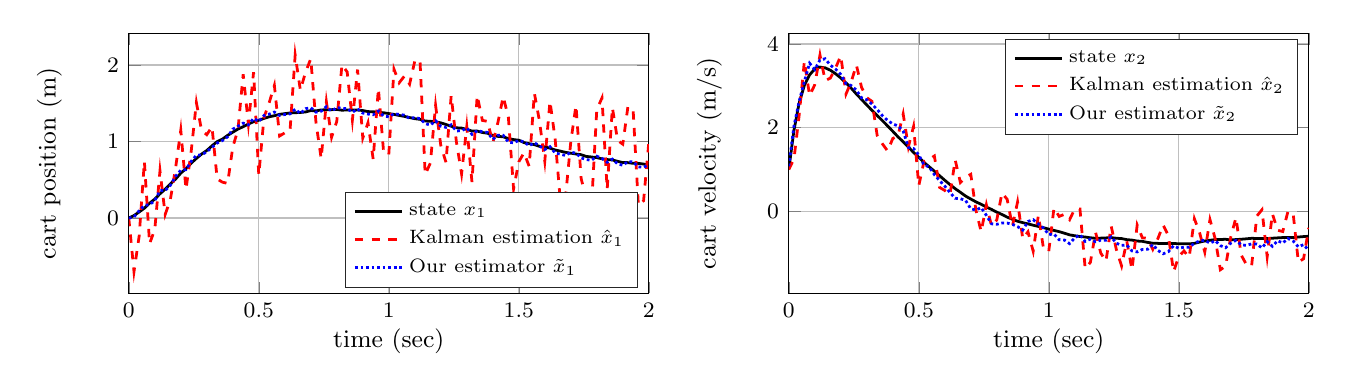
\begin{tikzpicture}
\begin{axis}
[	width=2.6in,
	height=1.3in,
	at={(0in,1.7in)},
	scale only axis,
	xmin=0,
	xmax=2.0,
	xlabel={\small time (sec)},
	ylabel={\small cart position (m)},
	x label style={at={(axis description cs:0.5,-0.1)},anchor=north},
	y label style={at={(axis description cs:-0.11,.5)},anchor=south},
	xticklabel style = {font=\footnotesize},
	yticklabel style = {font=\footnotesize},
	axis background/.style={fill=white},
	xmajorgrids,
	ymajorgrids,
	legend style={at={(0.98,0.02)}, anchor=south east, legend cell align=left, align=left, draw=white!15!black, font=\scriptsize}]
	 \addplot [color={black}, line width=1pt]
	table[row sep={\\}]
	{
0.0  0.0  \\
0.02  0.0312885282018752  \\
0.04  0.0788123875203588  \\
0.06  0.12783983276693056  \\
0.08  0.19302443002512482  \\
0.1  0.24691171369130704  \\
0.12  0.3161471924463811  \\
0.14  0.37655820357754827  \\
0.16  0.44574118653184464  \\
0.18  0.508717686134174  \\
0.2  0.5858944594685165  \\
0.22  0.6442080290694358  \\
0.24  0.7170003106288797  \\
0.26  0.7781390817476541  \\
0.28  0.8348607428170365  \\
0.3  0.8820850124163883  \\
0.32  0.9429843329186438  \\
0.34  0.9985281560618742  \\
0.36  1.0302635273555911  \\
0.38  1.0791321889652439  \\
0.4  1.121245022981027  \\
0.42  1.161891300602804  \\
0.44  1.192700117051156  \\
0.46  1.2287933108791957  \\
0.48  1.2579103583060975  \\
0.5  1.2769090558718827  \\
0.52  1.3010074939994656  \\
0.54  1.322606952127935  \\
0.56  1.3363739300408208  \\
0.58  1.3547060181087645  \\
0.6  1.3637156124358794  \\
0.62  1.372208147950066  \\
0.64  1.3758158415504202  \\
0.66  1.3789775570173455  \\
0.68  1.3858658992171147  \\
0.7  1.4038540774769968  \\
0.72  1.399388270372787  \\
0.74  1.4121158471937587  \\
0.76  1.413967536880243  \\
0.78  1.4159014376757404  \\
0.8  1.417828678620937  \\
0.82  1.408439121962671  \\
0.84  1.4119812043541529  \\
0.86  1.4115583441626582  \\
0.88  1.4107211138008886  \\
0.9  1.4043543531943106  \\
0.92  1.390269579268504  \\
0.94  1.388444098074998  \\
0.96  1.3811571553361286  \\
0.98  1.375136659753237  \\
1.0  1.3650405410205926  \\
1.02  1.3532746327113854  \\
1.04  1.3399687394128827  \\
1.06  1.3274222529638806  \\
1.08  1.312887237057181  \\
1.1  1.297953855938006  \\
1.12  1.2888243656725031  \\
1.14  1.2671580891040044  \\
1.16  1.2636596712198738  \\
1.18  1.2568123705161265  \\
1.2  1.2433534208208616  \\
1.22  1.222018058868546  \\
1.24  1.199082947901861  \\
1.26  1.1789132315105741  \\
1.28  1.1746923163614416  \\
1.3  1.1574829037716936  \\
1.32  1.1356654326585793  \\
1.34  1.1362230591177622  \\
1.36  1.1171876047888512  \\
1.38  1.1074990138885137  \\
1.4  1.078974551777622  \\
1.42  1.0661973181301283  \\
1.44  1.0609127088404313  \\
1.46  1.0372993334160026  \\
1.48  1.024440355201395  \\
1.5  1.016773165435164  \\
1.52  0.985372726177421  \\
1.54  0.9708403750356196  \\
1.56  0.9591509832628655  \\
1.58  0.9355856912687716  \\
1.6  0.9288408011304456  \\
1.62  0.9124527452153604  \\
1.64  0.888692309701688  \\
1.66  0.8736279796836832  \\
1.68  0.8576149131794482  \\
1.7  0.8467338065845937  \\
1.72  0.8357323419078908  \\
1.74  0.8271295129691318  \\
1.76  0.804168519172342  \\
1.78  0.7973787024419723  \\
1.8  0.7885831880803513  \\
1.82  0.7731913576797228  \\
1.84  0.7632841476573989  \\
1.86  0.7581919965043644  \\
1.88  0.7404424073275442  \\
1.9  0.7242330930938433  \\
1.92  0.7232652267292055  \\
1.94  0.7141451711559598  \\
1.96  0.7135626060421556  \\
1.98  0.7050839449630739  \\
2.0  0.6894219585423397  \\
	}
	;\addlegendentry{state $x_1$}
	
	\addplot [color={red},dashed, line width=1pt]
	table[row sep={\\}]
	{
 0.0  0.0  \\
0.02  -0.7016326820685982  \\
0.04  -0.23585571586261345  \\
0.06  0.7396609099297807  \\
0.08  -0.33621243440965815  \\
0.1  -0.15048791253219151  \\
0.12  0.6176826620511138  \\
0.14  0.04578213612712215  \\
0.16  0.24085153712000212  \\
0.18  0.6519749416537854  \\
0.2  1.1481340088757428  \\
0.22  0.3739654072288668  \\
0.24  0.8695195317551777  \\
0.26  1.5079986424406817  \\
0.28  1.1437489242746022  \\
0.3  1.0884297575593251  \\
0.32  1.192645206389877  \\
0.34  0.5096949773855692  \\
0.36  0.4682016134464051  \\
0.38  0.45158731684792996  \\
0.4  0.9245292733660191  \\
0.42  1.1563184823107087  \\
0.44  1.8782643853325425  \\
0.46  1.2286200415610418  \\
0.48  1.90560288844914  \\
0.5  0.5609048675886162  \\
0.52  1.314072432246385  \\
0.54  1.506294966924829  \\
0.56  1.732157136746129  \\
0.58  1.0713638460394828  \\
0.6  1.1124754014038012  \\
0.62  1.1325698189447386  \\
0.64  2.1299447613993494  \\
0.66  1.6694764974183034  \\
0.68  1.9074552913612985  \\
0.7  2.0802230570514464  \\
0.72  1.249075947340938  \\
0.74  0.7755524566336746  \\
0.76  1.5186582695973136  \\
0.78  1.053934096560571  \\
0.8  1.263845037327248  \\
0.82  2.004341804511319  \\
0.84  1.9076177543863433  \\
0.86  1.2791803217886837  \\
0.88  1.9388924541370987  \\
0.9  1.044856742034207  \\
0.92  1.2434718255294455  \\
0.94  0.7678933158489609  \\
0.96  1.6943045521016002  \\
0.98  0.8649726988503483  \\
1.0  0.826956736056349  \\
1.02  1.9441067890112704  \\
1.04  1.7671483990223398  \\
1.06  1.8537757329684719  \\
1.08  1.74869596272442  \\
1.1  2.050331385127062  \\
1.12  2.065323459242827  \\
1.14  0.5675645417737036  \\
1.16  0.7183137980272856  \\
1.18  1.4721749444770658  \\
1.2  0.9486696263681218  \\
1.22  0.7275878036994118  \\
1.24  1.5982571538598647  \\
1.26  0.9968108122528502  \\
1.28  0.5771790217717717  \\
1.3  1.1939220530371921  \\
1.32  0.4705513491038608  \\
1.34  1.6017654267607948  \\
1.36  1.2754776607476657  \\
1.38  1.2618686905389338  \\
1.4  0.9821092898946824  \\
1.42  1.2520370722954877  \\
1.44  1.5868463335267238  \\
1.46  1.315316213744334  \\
1.48  0.3809467176356255  \\
1.5  0.7343497684517054  \\
1.52  0.8525011066231617  \\
1.54  0.6747786775563649  \\
1.56  1.631306074588672  \\
1.58  1.259238093266994  \\
1.6  0.7406502576917274  \\
1.62  1.5270858735962223  \\
1.64  1.0273604220689518  \\
1.66  0.22013248694006454  \\
1.68  0.2814102904932267  \\
1.7  0.9937623709318437  \\
1.72  1.4722659204159319  \\
1.74  0.513230720725658  \\
1.76  0.24399096723995706  \\
1.78  0.17209686923052656  \\
1.8  1.414894962085707  \\
1.82  1.5689427180553022  \\
1.84  0.3738299073894682  \\
1.86  1.4432830585706296  \\
1.88  1.0146304626081781  \\
1.9  0.9646143450049791  \\
1.92  1.4599263074280486  \\
1.94  1.3992941378715475  \\
1.96  0.16577497949085318  \\
1.98  0.2250988953546872  \\
2.0  0.9813678260080361  \\
	}
	;\addlegendentry{{ Kalman estimation $\hat{x}_1$}}
    \addplot[densely dotted, color={blue}, line width=1pt]
        table[row sep={\\}]
        {
  0.0  -0.0016546478915138397  \\
0.02  0.012803800843751626  \\
0.04  0.09554688470489497  \\
0.06  0.16253616814154492  \\
0.08  0.1757155439630189  \\
0.1  0.22684144474391166  \\
0.12  0.3588610317373191  \\
0.14  0.3600565285670698  \\
0.16  0.4268314405275966  \\
0.18  0.5444687411092691  \\
0.2  0.6240844791843322  \\
0.22  0.6314795408897524  \\
0.24  0.7400311038559425  \\
0.26  0.8189832083536872  \\
0.28  0.8244024397244267  \\
0.3  0.8663905052304092  \\
0.32  0.922990301770209  \\
0.34  0.9798892619734936  \\
0.36  1.0117967230429303  \\
0.38  1.0599172908675325  \\
0.4  1.1603643852567949  \\
0.42  1.1990802015445396  \\
0.44  1.2395813207698205  \\
0.46  1.2165585171583397  \\
0.48  1.3013264919921557  \\
0.5  1.2609307571835484  \\
0.52  1.3386884784369582  \\
0.54  1.357083577925525  \\
0.56  1.3842326654411976  \\
0.58  1.3398267024517447  \\
0.6  1.3518845191939897  \\
0.62  1.3605004189076775  \\
0.64  1.4219380480003003  \\
0.66  1.3649203285273799  \\
0.68  1.4285890406210218  \\
0.7  1.4410836824050024  \\
0.72  1.3826840414912316  \\
0.74  1.3959236008102323  \\
0.76  1.4552823453620856  \\
0.78  1.3959039513270748  \\
0.8  1.4438071511837156  \\
0.82  1.432844078488602  \\
0.84  1.4299867320429205  \\
0.86  1.3813759762529558  \\
0.88  1.4265818351347233  \\
0.9  1.3709250480900586  \\
0.92  1.3579677545976403  \\
0.94  1.3487742263587437  \\
0.96  1.3975588490058366  \\
0.98  1.33454216140927  \\
1.0  1.3216205976334596  \\
1.02  1.3624960268492265  \\
1.04  1.353311126347017  \\
1.06  1.3439501738480442  \\
1.08  1.301369848305021  \\
1.1  1.3125870668179422  \\
1.12  1.2980724796332295  \\
1.14  1.2338677686687103  \\
1.16  1.2137553744273737  \\
1.18  1.2709021953976292  \\
1.2  1.1992025218793143  \\
1.22  1.183697398088326  \\
1.24  1.218570516572107  \\
1.26  1.137563007619231  \\
1.28  1.1405022675978889  \\
1.3  1.1765535132579692  \\
1.32  1.0928758663920797  \\
1.34  1.1414652285997844  \\
1.36  1.1271940964802922  \\
1.38  1.1178376669643972  \\
1.4  1.0277986083364172  \\
1.42  1.0805816091531892  \\
1.44  1.0807849167204544  \\
1.46  0.9920763178114405  \\
1.48  0.9817306703518764  \\
1.5  1.0134477693156418  \\
1.52  0.9951974251474277  \\
1.54  0.9442285914088713  \\
1.56  0.9833197436088972  \\
1.58  0.9409151710618642  \\
1.6  0.8946300833123895  \\
1.62  0.9316112622492073  \\
1.64  0.8489701821077618  \\
1.66  0.8339106994871763  \\
1.68  0.8161789446932478  \\
1.7  0.859266662119662  \\
1.72  0.8476876655078228  \\
1.74  0.7855933449829767  \\
1.76  0.7624117087703305  \\
1.78  0.7551194589099179  \\
1.8  0.8077894968082772  \\
1.82  0.7782348664563057  \\
1.84  0.7291031405864548  \\
1.86  0.7692963458943343  \\
1.88  0.7074919875254148  \\
1.9  0.6891930843264874  \\
1.92  0.7372792789114803  \\
1.94  0.7335083478070233  \\
1.96  0.668317016120237  \\
1.98  0.6637710011872  \\
2.0  0.6980071501144504  \\
        }
        ;\addlegendentry{{ Our estimator $\tilde{x}_1$}}
        
\end{axis}

\begin{axis}
[	width=2.6in,
height=1.3in,
at={(3.3in,1.7in)},
scale only axis,
xmin=0,
xmax=2.0,
xlabel={\small time (sec)},
ylabel={\small cart velocity (m/s)},
x label style={at={(axis description cs:0.5,-0.1)},anchor=north},
y label style={at={(axis description cs:-0.11,.5)},anchor=south},
xticklabel style = {font=\footnotesize},
yticklabel style = {font=\footnotesize},
axis background/.style={fill=white},
xmajorgrids,
ymajorgrids,
legend style={at={(0.98,0.98)}, anchor=north east, legend cell align=left, align=left, draw=white!15!black, font=\scriptsize}]
\addplot [color={black}, line width=1pt]
table[row sep={\\}]
{
0.0  1.0  \\
0.02  1.9391209237895848  \\
0.04  2.590989465213296  \\
0.06  3.0112038136322097  \\
0.08  3.262145933341507  \\
0.1  3.404055223712122  \\
0.12  3.448329465319425  \\
0.14  3.4304868325634814  \\
0.16  3.372844199991032  \\
0.18  3.289148790648013  \\
0.2  3.1885535486300065  \\
0.22  3.0692926604120068  \\
0.24  2.944939735179303  \\
0.26  2.8041012335303797  \\
0.28  2.6741250131880947  \\
0.3  2.542186317426113  \\
0.32  2.4133137843864088  \\
0.34  2.2902036362827154  \\
0.36  2.1676068541377513  \\
0.38  2.041575453393154  \\
0.4  1.912003547154351  \\
0.42  1.7805111075137916  \\
0.44  1.6613280032011057  \\
0.46  1.5367336043391617  \\
0.48  1.4056656658012763  \\
0.5  1.290973151946963  \\
0.52  1.1679927469559728  \\
0.54  1.0638319121527307  \\
0.56  0.9574423074532515  \\
0.58  0.8490799761838703  \\
0.6  0.7412336946439754  \\
0.62  0.6375781972725671  \\
0.64  0.5397855090185257  \\
0.66  0.4532142587467182  \\
0.68  0.36280368622739734  \\
0.7  0.2917937269950741  \\
0.72  0.22364279659665026  \\
0.74  0.16641956056250445  \\
0.76  0.09957734983786248  \\
0.78  0.04285943612658093  \\
0.8  -0.021996866697433476  \\
0.82  -0.07785062469992182  \\
0.84  -0.14179940204160668  \\
0.86  -0.192111834507433  \\
0.88  -0.2395799342971533  \\
0.9  -0.2731098299450826  \\
0.92  -0.3023493674467045  \\
0.94  -0.33494599088485866  \\
0.96  -0.3634837919419665  \\
0.98  -0.39429252436904916  \\
1.0  -0.427376069393288  \\
1.02  -0.45849247351460987  \\
1.04  -0.4886944820743368  \\
1.06  -0.5253851993311534  \\
1.08  -0.5650389302187308  \\
1.1  -0.5863884385696589  \\
1.12  -0.6038458947549443  \\
1.14  -0.6171167795918366  \\
1.16  -0.6349431570995152  \\
1.18  -0.6474517267585185  \\
1.2  -0.6434772685824866  \\
1.22  -0.6379941265376432  \\
1.24  -0.6322982024232  \\
1.26  -0.6458598128233805  \\
1.28  -0.654065958989119  \\
1.3  -0.679509056048515  \\
1.32  -0.6905768067028223  \\
1.34  -0.7130004889104322  \\
1.36  -0.7203615215047533  \\
1.38  -0.7454102026881453  \\
1.4  -0.7645886120566366  \\
1.42  -0.7688770436773459  \\
1.44  -0.7733996969520899  \\
1.46  -0.767714095270773  \\
1.48  -0.7704943594144114  \\
1.5  -0.7792436303557043  \\
1.52  -0.7763125311369948  \\
1.54  -0.7800818638691298  \\
1.56  -0.7683618200545922  \\
1.58  -0.7379645382430333  \\
1.6  -0.7120211968404369  \\
1.62  -0.6944313784107807  \\
1.64  -0.6788356905664363  \\
1.66  -0.6755209780869861  \\
1.68  -0.6713863855448137  \\
1.7  -0.6861143109771883  \\
1.72  -0.6777605242430396  \\
1.74  -0.67008745456601  \\
1.76  -0.6595296803854034  \\
1.78  -0.6480090140165278  \\
1.8  -0.651450136105128  \\
1.82  -0.6517143018493359  \\
1.84  -0.6525749963680775  \\
1.86  -0.6453041999310413  \\
1.88  -0.6373422062650471  \\
1.9  -0.630057062238385  \\
1.92  -0.6301433102561566  \\
1.94  -0.6297353309511714  \\
1.96  -0.616497720752044  \\
1.98  -0.6064299270620612  \\
2.0  -0.5981417131472986  \\
}
;\addlegendentry{state $x_2$}

\addplot [color={red},dashed, line width=1pt]
table[row sep={\\}]
{
   0.0  1.0  \\
0.02  1.2520375776998334  \\
0.04  2.300009604013391  \\
0.06  3.592060558953479  \\
0.08  2.7649250252416024  \\
0.1  3.0262809894865192  \\
0.12  3.737499294098212  \\
0.14  3.12110372825729  \\
0.16  3.1861891324106963  \\
0.18  3.4274138963467804  \\
0.2  3.7198764070873898  \\
0.22  2.803236665480386  \\
0.24  3.0913857467081614  \\
0.26  3.500316410919404  \\
0.28  2.961819884446753  \\
0.3  2.7158798761007077  \\
0.32  2.628985356939085  \\
0.34  1.812881338210877  \\
0.36  1.613351795096433  \\
0.38  1.4425020734693912  \\
0.4  1.7399265201110468  \\
0.42  1.8028149398680218  \\
0.44  2.326401112633281  \\
0.46  1.5423332185675656  \\
0.48  2.0287784649248946  \\
0.5  0.6102389896017371  \\
0.52  1.191268735603829  \\
0.54  1.237764042431899  \\
0.56  1.3224531999777234  \\
0.58  0.5704468281498346  \\
0.6  0.49673279383399516  \\
0.62  0.3981857887619049  \\
0.64  1.229096741477517  \\
0.66  0.6877935606365496  \\
0.68  0.8141279419565274  \\
0.7  0.8835958773833297  \\
0.72  0.020568475438498934  \\
0.74  -0.48943871844095244  \\
0.76  0.15514500137660914  \\
0.78  -0.35244027450211646  \\
0.8  -0.20815875770989178  \\
0.82  0.438027801028096  \\
0.84  0.2843113304577627  \\
0.86  -0.36055354865939027  \\
0.88  0.22295697043163942  \\
0.9  -0.6589673240118565  \\
0.92  -0.49078963983506707  \\
0.94  -0.9568518427371487  \\
0.96  -0.09412376172945769  \\
0.98  -0.9039459953155622  \\
1.0  -0.9563233110889232  \\
1.02  0.07966430313712625  \\
1.04  -0.12380509206160606  \\
1.06  -0.07402619999655324  \\
1.08  -0.2030130407085846  \\
1.1  0.056772989288457865  \\
1.12  0.052243394850999936  \\
1.14  -1.3723270099750198  \\
1.16  -1.223561027584351  \\
1.18  -0.5057712567390962  \\
1.2  -1.0011869394094126  \\
1.22  -1.1949065410616595  \\
1.24  -0.3549026777961153  \\
1.26  -0.9183435604352458  \\
1.28  -1.3080548317301632  \\
1.3  -0.7141746173316741  \\
1.32  -1.40188819595665  \\
1.34  -0.32959480344887826  \\
1.36  -0.6367413723090429  \\
1.38  -0.6468663524250073  \\
1.4  -0.9123046246791389  \\
1.42  -0.6493285146517109  \\
1.44  -0.3288712775744558  \\
1.46  -0.5838383248759282  \\
1.48  -1.4457255354947045  \\
1.5  -1.081487548739723  \\
1.52  -0.9510426624820778  \\
1.54  -1.1035250307171802  \\
1.56  -0.17920451360073142  \\
1.58  -0.5104956175392936  \\
1.6  -0.9774753425770938  \\
1.62  -0.20198433902106339  \\
1.64  -0.6568916513437502  \\
1.66  -1.400750886670715  \\
1.68  -1.3131253278757518  \\
1.7  -0.615670432340711  \\
1.72  -0.15068321641309024  \\
1.74  -1.046636962700916  \\
1.76  -1.2754309384409042  \\
1.78  -1.3185154829093082  \\
1.8  -0.11618707527794592  \\
1.82  0.03486447792739433  \\
1.84  -1.0885087582132544  \\
1.86  -0.05963010563322024  \\
1.88  -0.4554360354252778  \\
1.9  -0.48533050983918957  \\
1.92  -0.004104539990258171  \\
1.94  -0.05907869157379575  \\
1.96  -1.2193817306049763  \\
1.98  -1.1368577322583464  \\
2.0  -0.39764266241265944  \\
}
;\addlegendentry{{ Kalman estimation $\hat{x}_2$}}
\addplot[densely dotted, color={blue}, line width=1pt]
table[row sep={\\}]
{
 0.0  1.0766943557990734  \\
0.02  2.0402360299618394  \\
0.04  2.6309454758292494  \\
0.06  3.1068675196902764  \\
0.08  3.54080134552669  \\
0.1  3.390423831584909  \\
0.12  3.6176773435075993  \\
0.14  3.6483302835825806  \\
0.16  3.4940837403221066  \\
0.18  3.400518174132703  \\
0.2  3.272179041445286  \\
0.22  3.051182580312056  \\
0.24  3.007136640276949  \\
0.26  2.89668735820574  \\
0.28  2.713233393415006  \\
0.3  2.666081620611238  \\
0.32  2.562083551484879  \\
0.34  2.434075387513464  \\
0.36  2.286871848307895  \\
0.38  2.1725112918581857  \\
0.4  2.0891911107037067  \\
0.42  2.0406855463131692  \\
0.44  1.9222977654197195  \\
0.46  1.5257739757194784  \\
0.48  1.4989888926426562  \\
0.5  1.3473304530955497  \\
0.52  1.109572133570126  \\
0.54  1.0592201977960447  \\
0.56  0.8758454837144379  \\
0.58  0.7337559238480325  \\
0.6  0.6004573856743581  \\
0.62  0.44824465603343244  \\
0.64  0.3101689801671155  \\
0.66  0.2987946638154928  \\
0.68  0.2600433017728896  \\
0.7  0.05672463712827543  \\
0.72  0.030413094277216744  \\
0.74  0.08555028416184272  \\
0.76  -0.09971583953501285  \\
0.78  -0.3017142438245463  \\
0.8  -0.3122042796770449  \\
0.82  -0.2827534315188673  \\
0.84  -0.2829505347667381  \\
0.86  -0.31444525280989494  \\
0.88  -0.3679083896574561  \\
0.9  -0.4523096410930004  \\
0.92  -0.24528076875533894  \\
0.94  -0.2012204257573242  \\
0.96  -0.30459353150941115  \\
0.98  -0.4034606060932498  \\
1.0  -0.5579468081734421  \\
1.02  -0.5456885041145905  \\
1.04  -0.6834788869342028  \\
1.06  -0.6876029558751029  \\
1.08  -0.7754242277751354  \\
1.1  -0.6357568393571198  \\
1.12  -0.5647630895137999  \\
1.14  -0.722224950479285  \\
1.16  -0.6672023210232  \\
1.18  -0.730160044324085  \\
1.2  -0.6932767721446531  \\
1.22  -0.6955416637290003  \\
1.24  -0.6148744413228993  \\
1.26  -0.7646738905171426  \\
1.28  -0.8174879195874942  \\
1.3  -0.8086440314412106  \\
1.32  -0.9489524673668117  \\
1.34  -0.9731834368682155  \\
1.36  -0.9134270631253525  \\
1.38  -0.9095082237264895  \\
1.4  -0.7968292615369957  \\
1.42  -0.9388984989978707  \\
1.44  -1.0175358467975835  \\
1.46  -0.9680022103203125  \\
1.48  -0.8260065615129651  \\
1.5  -0.886260333768104  \\
1.52  -0.8603670806734103  \\
1.54  -0.8640190493688218  \\
1.56  -0.7640364116753472  \\
1.58  -0.7120111509452782  \\
1.6  -0.6936300126424111  \\
1.62  -0.764741414382075  \\
1.64  -0.7033854196176764  \\
1.66  -0.8226871876980503  \\
1.68  -0.8731757555208807  \\
1.7  -0.7626857480875107  \\
1.72  -0.6967479415177407  \\
1.74  -0.8031387793448946  \\
1.76  -0.8170700823758712  \\
1.78  -0.7816777307010934  \\
1.8  -0.7845261659077962  \\
1.82  -0.8770371475311388  \\
1.84  -0.7264585052225073  \\
1.86  -0.8394900475907195  \\
1.88  -0.705278834141262  \\
1.9  -0.760571799602993  \\
1.92  -0.650966035713089  \\
1.94  -0.7135157071013508  \\
1.96  -0.8527263663135067  \\
1.98  -0.7989930114769055  \\
2.0  -0.9373767100494399  \\
}
;\addlegendentry{{ Our estimator $\tilde{x}_2$}}

\end{axis}

%  	\begin{axis}
%	[	width=2.6in,
%	height=1.3in,
%	at={(0in,0in)},
%	scale only axis,
%	xmin=0,
%	xmax=2.0,
%%	ymin=-4,
%%	ymax=2,
%	xlabel={\small time (sec)},
%	ylabel={\small $x_3$ pendulumn angle},
%	x label style={at={(axis description cs:0.5,-0.1)},anchor=north},
%	y label style={at={(axis description cs:-0.11,.5)},anchor=south},
%	xticklabel style = {font=\footnotesize},
%	yticklabel style = {font=\footnotesize},
%	axis background/.style={fill=white},
%	xmajorgrids,
%	ymajorgrids,
%	legend style={at={(0.98,0.02)}, anchor=south east, legend cell align=left, align=left, draw=white!15!black, font=\scriptsize}]
%	\addplot [color={black}, line width=1pt]
%	table[row sep={\\}]
%	{
%0.0  0.0  \\
%0.02  0.00772853593415913  \\
%0.04  0.004801671416923327  \\
%0.06  -0.012528997431996048  \\
%0.08  -0.034478619332425936  \\
%0.1  -0.06220231524500317  \\
%0.12  -0.08812635048651297  \\
%0.14  -0.11408845091735348  \\
%0.16  -0.14488997218330013  \\
%0.18  -0.16947348245078697  \\
%0.2  -0.19501471373927462  \\
%0.22  -0.2166030568036244  \\
%0.24  -0.23694887645664164  \\
%0.26  -0.2534179553657174  \\
%0.28  -0.2659048131170473  \\
%0.3  -0.2814074322954603  \\
%0.32  -0.2947651384686937  \\
%0.34  -0.30280625979339526  \\
%0.36  -0.3110461733895194  \\
%0.38  -0.322599925444607  \\
%0.4  -0.3266601375700984  \\
%0.42  -0.32832183302190043  \\
%0.44  -0.33079378651792585  \\
%0.46  -0.33139999061403563  \\
%0.48  -0.33190912976035625  \\
%0.5  -0.32830514918189446  \\
%0.52  -0.3265624628054656  \\
%0.54  -0.3231032971609128  \\
%0.56  -0.31943423376946206  \\
%0.58  -0.31567219360956844  \\
%0.6  -0.3139459878003922  \\
%0.62  -0.30858429971742735  \\
%0.64  -0.302866065490615  \\
%0.66  -0.2975240107704187  \\
%0.68  -0.29156813130488785  \\
%0.7  -0.28705864201984305  \\
%0.72  -0.2800613967051828  \\
%0.74  -0.2721345042496352  \\
%0.76  -0.2675647476463787  \\
%0.78  -0.26004373544306775  \\
%0.8  -0.24895562242482422  \\
%0.82  -0.24469615255703123  \\
%0.84  -0.23679296240647962  \\
%0.86  -0.22526462977535064  \\
%0.88  -0.21530137387528134  \\
%0.9  -0.2019610820610649  \\
%0.92  -0.19283115640996426  \\
%0.94  -0.18404650174938508  \\
%0.96  -0.1761938176509628  \\
%0.98  -0.16952154188571567  \\
%1.0  -0.16068318494400077  \\
%1.02  -0.15115385465801076  \\
%1.04  -0.142077499764086  \\
%1.06  -0.13285231555738442  \\
%1.08  -0.12217488148841449  \\
%1.1  -0.11717625074624005  \\
%1.12  -0.11014342489808715  \\
%1.14  -0.10290962697247244  \\
%1.16  -0.09707223606283309  \\
%1.18  -0.08535583686102192  \\
%1.2  -0.07985586728850495  \\
%1.22  -0.07053290137389215  \\
%1.24  -0.0660756875734225  \\
%1.26  -0.05925950423578198  \\
%1.28  -0.04983238664926049  \\
%1.3  -0.046321730532286276  \\
%1.32  -0.04111947230774583  \\
%1.34  -0.03716014124124552  \\
%1.36  -0.026958173254637667  \\
%1.38  -0.02105479624823502  \\
%1.4  -0.013204082238369545  \\
%1.42  -0.007208612852129617  \\
%1.44  -0.005029793064317797  \\
%1.46  -0.0030365387904538444  \\
%1.48  -0.004685191023569348  \\
%1.5  -0.0013502134977833556  \\
%1.52  -0.0012637857934116841  \\
%1.54  -0.0012840803221537893  \\
%1.56  0.004161592495718868  \\
%1.58  0.007337270321035059  \\
%1.6  0.007873265952081725  \\
%1.62  0.007756595504494869  \\
%1.64  0.012948213825993315  \\
%1.66  0.01713997304166258  \\
%1.68  0.019303428528959714  \\
%1.7  0.021720664071569973  \\
%1.72  0.021496525088056485  \\
%1.74  0.02269954427453162  \\
%1.76  0.025127263635035712  \\
%1.78  0.025581388241573386  \\
%1.8  0.022956371536018347  \\
%1.82  0.020320909246699284  \\
%1.84  0.02325727363447171  \\
%1.86  0.022566429135964905  \\
%1.88  0.025410932971556357  \\
%1.9  0.025581397517493814  \\
%1.92  0.024133015365711413  \\
%1.94  0.024607306183292644  \\
%1.96  0.02686997993370564  \\
%1.98  0.028618584557972122  \\
%2.0  0.02949612536857937  \\
%	}
%	;\addlegendentry{state $x_3$}
%	\addplot [color={red},dashed, line width=1pt]
%	table[row sep={\\}]
%	{
%	 0.0  0.0  \\
%	0.02  0.00809402453328914  \\
%	0.04  0.002283710058266839  \\
%	0.06  -0.011924222353404363  \\
%	0.08  -0.03538807548199385  \\
%	0.1  -0.062495688561897404  \\
%	0.12  -0.08979727756857352  \\
%	0.14  -0.11596912737252132  \\
%	0.16  -0.14427298978459968  \\
%	0.18  -0.1699091880689923  \\
%	0.2  -0.19571409358693093  \\
%	0.22  -0.21710723871475957  \\
%	0.24  -0.23750518798723996  \\
%	0.26  -0.2523487237267693  \\
%	0.28  -0.26564551359739796  \\
%	0.3  -0.28113924184632594  \\
%	0.32  -0.29344313265186917  \\
%	0.34  -0.30387742299429843  \\
%	0.36  -0.31093266172634626  \\
%	0.38  -0.32032314034771303  \\
%	0.4  -0.32488432492231156  \\
%	0.42  -0.328256133800731  \\
%	0.44  -0.33170684466667966  \\
%	0.46  -0.33284554813223155  \\
%	0.48  -0.32934060251669267  \\
%	0.5  -0.32881415681358606  \\
%	0.52  -0.32672393145274836  \\
%	0.54  -0.3217023284966502  \\
%	0.56  -0.31920782046530927  \\
%	0.58  -0.3155857583713461  \\
%	0.6  -0.31200171978648444  \\
%	0.62  -0.30753884981430435  \\
%	0.64  -0.30328744734313084  \\
%	0.66  -0.298819639225292  \\
%	0.68  -0.2916263924411364  \\
%	0.7  -0.2838538399639527  \\
%	0.72  -0.27822533107121034  \\
%	0.74  -0.27214850374295424  \\
%	0.76  -0.2649862125224101  \\
%	0.78  -0.2581935349054245  \\
%	0.8  -0.24687375692743166  \\
%	0.82  -0.24215334598492766  \\
%	0.84  -0.23463968652823464  \\
%	0.86  -0.2266454648618093  \\
%	0.88  -0.21570653361944153  \\
%	0.9  -0.20378113555698663  \\
%	0.92  -0.1922094272504351  \\
%	0.94  -0.18193892229656553  \\
%	0.96  -0.17462306148804935  \\
%	0.98  -0.16857998362472904  \\
%	1.0  -0.1589098101915298  \\
%	1.02  -0.1502282447377052  \\
%	1.04  -0.14310208638808308  \\
%	1.06  -0.13391428982914821  \\
%	1.08  -0.12206666034954945  \\
%	1.1  -0.11753381580332939  \\
%	1.12  -0.11064111898353321  \\
%	1.14  -0.10215982660161821  \\
%	1.16  -0.096618902112179  \\
%	1.18  -0.08817640412095815  \\
%	1.2  -0.07931844432254224  \\
%	1.22  -0.0713170158403937  \\
%	1.24  -0.06598326032462205  \\
%	1.26  -0.05869782541506201  \\
%	1.28  -0.05244831403760163  \\
%	1.3  -0.04689123976106053  \\
%	1.32  -0.04325454089798624  \\
%	1.34  -0.03885220256504527  \\
%	1.36  -0.030517495413270805  \\
%	1.38  -0.024466342268987945  \\
%	1.4  -0.018729185184462  \\
%	1.42  -0.010157661361933055  \\
%	1.44  -0.005799650225733364  \\
%	1.46  -0.0017710381011364653  \\
%	1.48  -0.002224799382994183  \\
%	1.5  -0.0037629560253844437  \\
%	1.52  -0.00020440203585928116  \\
%	1.54  0.0012643359647233753  \\
%	1.56  0.003252784378121404  \\
%	1.58  0.005266412443152401  \\
%	1.6  0.006949937595322902  \\
%	1.62  0.008256452575278935  \\
%	1.64  0.012007453507124496  \\
%	1.66  0.01615310418726861  \\
%	1.68  0.019000666804788804  \\
%	1.7  0.022087371511188413  \\
%	1.72  0.022261092399250972  \\
%	1.74  0.02355749395802008  \\
%	1.76  0.023895346270558754  \\
%	1.78  0.026333022304786253  \\
%	1.8  0.02456626556539792  \\
%	1.82  0.021605386228436392  \\
%	1.84  0.023528349423668403  \\
%	1.86  0.023572743261476937  \\
%	1.88  0.025126899283551846  \\
%	1.9  0.025833933274513415  \\
%	1.92  0.02280935517999988  \\
%	1.94  0.025189469054832925  \\
%	1.96  0.02661138935665535  \\
%	1.98  0.02763011362829756  \\
%	2.0  0.027469141828147026  \\
%	}
%	;\addlegendentry{{ Kalman estimation $\hat{x}_3$}}
%	\addplot[densely dotted, color={blue}, line width=1pt]
%	table[row sep={\\}]
%	{
%    0.0  1.8153964737662312e-5  \\
%0.02  0.0066894619554046355  \\
%0.04  0.0018375871994040162  \\
%0.06  -0.011012697570773474  \\
%0.08  -0.03609804873935931  \\
%0.1  -0.06340645502442915  \\
%0.12  -0.0895457918792631  \\
%0.14  -0.11546107462068377  \\
%0.16  -0.14461477831571443  \\
%0.18  -0.17007154514361927  \\
%0.2  -0.1965051643232883  \\
%0.22  -0.2166340902306285  \\
%0.24  -0.23770039325448397  \\
%0.26  -0.2507335125541037  \\
%0.28  -0.2645156857629006  \\
%0.3  -0.28216527675191616  \\
%0.32  -0.2939902057265568  \\
%0.34  -0.30440857374041375  \\
%0.36  -0.31047444062583235  \\
%0.38  -0.32198495278139255  \\
%0.4  -0.3249118700086211  \\
%0.42  -0.32841640163734204  \\
%0.44  -0.33251010788936297  \\
%0.46  -0.3331188005365526  \\
%0.48  -0.32767165979082796  \\
%0.5  -0.3288637216034393  \\
%0.52  -0.3265504673964966  \\
%0.54  -0.3205275268798475  \\
%0.56  -0.3197884422608594  \\
%0.58  -0.3157679939079811  \\
%0.6  -0.31254421435944685  \\
%0.62  -0.30806083114358135  \\
%0.64  -0.3038352148338218  \\
%0.66  -0.2994116819525727  \\
%0.68  -0.29121889287466646  \\
%0.7  -0.2833617882231757  \\
%0.72  -0.27936861590095097  \\
%0.74  -0.27290542088826425  \\
%0.76  -0.2654318394097727  \\
%0.78  -0.25942935600796185  \\
%0.8  -0.2457658293296008  \\
%0.82  -0.24403414344605018  \\
%0.84  -0.2358616914531913  \\
%0.86  -0.2275077308550984  \\
%0.88  -0.21485981313066116  \\
%0.9  -0.20232178782749977  \\
%0.92  -0.19104608352709898  \\
%0.94  -0.18111885006671183  \\
%0.96  -0.1754534261052666  \\
%0.98  -0.17003134488456753  \\
%1.0  -0.15878283143959224  \\
%1.02  -0.15051065091807594  \\
%1.04  -0.1435009071579159  \\
%1.06  -0.13363074186982313  \\
%1.08  -0.12038778178826819  \\
%1.1  -0.11866338138681089  \\
%1.12  -0.110930248968576  \\
%1.14  -0.10181163345285733  \\
%1.16  -0.09751700179946482  \\
%1.18  -0.08758702035485068  \\
%1.2  -0.07785509840417323  \\
%1.22  -0.07050311362538186  \\
%1.24  -0.06601841440192815  \\
%1.26  -0.05793710743206526  \\
%1.28  -0.051999353311811235  \\
%1.3  -0.04693730475850037  \\
%1.32  -0.04389217870983184  \\
%1.34  -0.038972560152190514  \\
%1.36  -0.02865888152011623  \\
%1.38  -0.02353592133370778  \\
%1.4  -0.017640744192343967  \\
%1.42  -0.007667707763960579  \\
%1.44  -0.004952961222438092  \\
%1.46  -0.0008037137317556581  \\
%1.48  -0.003445327891030425  \\
%1.5  -0.005518722706033974  \\
%1.52  0.0004546477429451413  \\
%1.54  0.0010515168391628813  \\
%1.56  0.0032978681139044274  \\
%1.58  0.005456467908684386  \\
%1.6  0.007016058115342972  \\
%1.62  0.007992613905111441  \\
%1.64  0.013215471326015648  \\
%1.66  0.01730891328170967  \\
%1.68  0.01980891940823777  \\
%1.7  0.023250483613783467  \\
%1.72  0.02194819975361911  \\
%1.74  0.023940958356646756  \\
%1.76  0.023721571245686246  \\
%1.78  0.027350023652804832  \\
%1.8  0.023546924861985615  \\
%1.82  0.019857344070720775  \\
%1.84  0.023909886569047793  \\
%1.86  0.0231294380862511  \\
%1.88  0.02574352864188202  \\
%1.9  0.025842587721728108  \\
%1.92  0.02092146538831675  \\
%1.94  0.025931184643444655  \\
%1.96  0.027084411024922466  \\
%1.98  0.027575839585923738  \\
%2.0  0.026971498895954696  \\
%	}
%;\addlegendentry{{our estimation $\tilde{x}_3$}}
%
%
%\end{axis}
%
%\begin{axis}
%[	width=2.6in,
%height=1.3in,
%at={(3.3in,0in)},
%scale only axis,
%xmin=0,
%xmax=2.0,
%%ymin=-4,
%%ymax=2,
%xlabel={\small time (sec)},
%ylabel={\small $x_4$ pendulumn angle velocity},
%x label style={at={(axis description cs:0.5,-0.1)},anchor=north},
%y label style={at={(axis description cs:-0.11,.5)},anchor=south},
%xticklabel style = {font=\footnotesize},
%yticklabel style = {font=\footnotesize},
%axis background/.style={fill=white},
%xmajorgrids,
%ymajorgrids,
%legend style={at={(0.98,0.02)}, anchor=south east, legend cell align=left, align=left, draw=white!15!black, font=\scriptsize}]
%\addplot [color={black}, line width=1pt]
%table[row sep={\\}]
%{
%  0.0  1.0  \\
%0.02  0.05313305390126177  \\
%0.04  -0.5807597079886778  \\
%0.06  -0.9849649892184913  \\
%0.08  -1.2236616544745775  \\
%0.1  -1.3448708265564777  \\
%0.12  -1.3911973425235322  \\
%0.14  -1.3847017109780744  \\
%0.16  -1.3360588370385862  \\
%0.18  -1.2612956960549269  \\
%0.2  -1.1712121233640451  \\
%0.22  -1.071999578445813  \\
%0.24  -0.9674797110228057  \\
%0.26  -0.8680549183886634  \\
%0.28  -0.7699884280336178  \\
%0.3  -0.6746842796248621  \\
%0.32  -0.586875654761506  \\
%0.34  -0.4959299174041296  \\
%0.36  -0.40597661697079446  \\
%0.38  -0.32771095994654365  \\
%0.4  -0.253961547290701  \\
%0.42  -0.18263871652089975  \\
%0.44  -0.11573407741218594  \\
%0.46  -0.05911515161120641  \\
%0.48  0.0009801138197992887  \\
%0.5  0.04463813200237973  \\
%0.52  0.09038368590143643  \\
%0.54  0.12381466371390598  \\
%0.56  0.16193471899976158  \\
%0.58  0.19217803962499197  \\
%0.6  0.2284585486584002  \\
%0.62  0.27315223526991256  \\
%0.64  0.3029744279918313  \\
%0.66  0.3360381761463694  \\
%0.68  0.36405311581028843  \\
%0.7  0.3862145241118462  \\
%0.72  0.4052381391063923  \\
%0.74  0.40659407112164414  \\
%0.76  0.4016463115722345  \\
%0.78  0.39680426743202124  \\
%0.8  0.3921338510569967  \\
%0.82  0.3884591608505884  \\
%0.84  0.3897778445333768  \\
%0.86  0.3978434385510643  \\
%0.88  0.40888248291393214  \\
%0.9  0.40349125898703586  \\
%0.92  0.4043181979298124  \\
%0.94  0.4001713487291486  \\
%0.96  0.397537790317619  \\
%0.98  0.3906342747298136  \\
%1.0  0.377882856254513  \\
%1.02  0.3727858562415341  \\
%1.04  0.3579748382263377  \\
%1.06  0.34457979003538486  \\
%1.08  0.3274365776280705  \\
%1.1  0.31223393396172927  \\
%1.12  0.2972605478138003  \\
%1.14  0.28374482940224277  \\
%1.16  0.27808313315371463  \\
%1.18  0.2752540519763583  \\
%1.2  0.27226461109496636  \\
%1.22  0.27696110635321103  \\
%1.24  0.26990768271144283  \\
%1.26  0.26054532527838425  \\
%1.28  0.2504740216554849  \\
%1.3  0.24312004848395827  \\
%1.32  0.24828658502523776  \\
%1.34  0.2471687742404289  \\
%1.36  0.2483512476352048  \\
%1.38  0.2421106054905815  \\
%1.4  0.2281155213543221  \\
%1.42  0.2192043397969218  \\
%1.44  0.21813440821530206  \\
%1.46  0.215847499113375  \\
%1.48  0.21810640903792972  \\
%1.5  0.21793606071633792  \\
%1.52  0.21839791991053367  \\
%1.54  0.21094224607272868  \\
%1.56  0.20175648284456538  \\
%1.58  0.18577552098976302  \\
%1.6  0.17234252915874954  \\
%1.62  0.1667589628096436  \\
%1.64  0.16336600936391402  \\
%1.66  0.15026901018454916  \\
%1.68  0.1427360828668787  \\
%1.7  0.13367410170858618  \\
%1.72  0.12734499958354706  \\
%1.74  0.11405351681196844  \\
%1.76  0.10587244286568445  \\
%1.78  0.10156266429081387  \\
%1.8  0.0936679758808678  \\
%1.82  0.08822122445956102  \\
%1.84  0.07018133601995245  \\
%1.86  0.05094537909202273  \\
%1.88  0.04130087142500513  \\
%1.9  0.032313361980953  \\
%1.92  0.02866897811479254  \\
%1.94  0.030018199155337016  \\
%1.96  0.029179914657290675  \\
%1.98  0.029178093401201616  \\
%2.0  0.02640041419686011  \\
%}
%;\addlegendentry{state $x_4$}
%\addplot [color={red},dashed, line width=1pt]
%table[row sep={\\}]
%{
%0.0  1.0  \\
%0.02  0.05196229099537668  \\
%0.04  -0.5824313535988286  \\
%0.06  -0.9891377715191895  \\
%0.08  -1.225040556372666  \\
%0.1  -1.3474376677420603  \\
%0.12  -1.3927650448471267  \\
%0.14  -1.3853875418228592  \\
%0.16  -1.3385535189542455  \\
%0.18  -1.2616908106226903  \\
%0.2  -1.1733481356619362  \\
%0.22  -1.0733971982561636  \\
%0.24  -0.9709048883726853  \\
%0.26  -0.8734509930998627  \\
%0.28  -0.7737477786715035  \\
%0.3  -0.6814462079764667  \\
%0.32  -0.5930068323706987  \\
%0.34  -0.5011111690344067  \\
%0.36  -0.4117486708366517  \\
%0.38  -0.32787217975647187  \\
%0.4  -0.25500615240975977  \\
%0.42  -0.18223637558459482  \\
%0.44  -0.1136859116043202  \\
%0.46  -0.05435490540626656  \\
%0.48  0.001052155333388885  \\
%0.5  0.047862836014496535  \\
%0.52  0.09307612385402939  \\
%0.54  0.12661541422593295  \\
%0.56  0.16673898540858903  \\
%0.58  0.20040364092746082  \\
%0.6  0.2378257684031066  \\
%0.62  0.28092995786664526  \\
%0.64  0.30722850104675375  \\
%0.66  0.33988761950874746  \\
%0.68  0.3717014698259486  \\
%0.7  0.39114473419457757  \\
%0.72  0.41074056965705785  \\
%0.74  0.4157082365437478  \\
%0.76  0.4107206907578836  \\
%0.78  0.40479797621004415  \\
%0.8  0.4002479612239634  \\
%0.82  0.39670525295180864  \\
%0.84  0.402980720989716  \\
%0.86  0.40966660580558506  \\
%0.88  0.41939855229643713  \\
%0.9  0.4136774603389678  \\
%0.92  0.41337706589827294  \\
%0.94  0.4076360923733703  \\
%0.96  0.40419133912255345  \\
%0.98  0.39738214224816115  \\
%1.0  0.38613613596819135  \\
%1.02  0.37863833492291044  \\
%1.04  0.3613171630485197  \\
%1.06  0.34817084130208276  \\
%1.08  0.3337665386001098  \\
%1.1  0.322513876054837  \\
%1.12  0.30951293238535926  \\
%1.14  0.29822140789925367  \\
%1.16  0.2887209415996951  \\
%1.18  0.2855447198327156  \\
%1.2  0.2792019100681843  \\
%1.22  0.28259480121327957  \\
%1.24  0.27674766540821855  \\
%1.26  0.2679337895584435  \\
%1.28  0.25957147095312993  \\
%1.3  0.2512852868921737  \\
%1.32  0.25335034594023265  \\
%1.34  0.2517049563980485  \\
%1.36  0.24854241554762116  \\
%1.38  0.2437570887642059  \\
%1.4  0.232081337423728  \\
%1.42  0.2246763936573522  \\
%1.44  0.22593853025256636  \\
%1.46  0.22180580292165525  \\
%1.48  0.2201777881736648  \\
%1.5  0.21772174841998373  \\
%1.52  0.22039359761167476  \\
%1.54  0.21451665272588324  \\
%1.56  0.20671496543671092  \\
%1.58  0.19237907013470915  \\
%1.6  0.17849341727408496  \\
%1.62  0.1693669711801831  \\
%1.64  0.1654694365161853  \\
%1.66  0.15476608715270937  \\
%1.68  0.14644491458503275  \\
%1.7  0.1380087312073818  \\
%1.72  0.12999696162763208  \\
%1.74  0.11642996712779241  \\
%1.76  0.10651977489569771  \\
%1.78  0.09914327961373791  \\
%1.8  0.09326070775598083  \\
%1.82  0.08760116773835838  \\
%1.84  0.07441328030636729  \\
%1.86  0.0534154762075595  \\
%1.88  0.04537417203289343  \\
%1.9  0.03311477519912949  \\
%1.92  0.029386264188961075  \\
%1.94  0.031449452742925314  \\
%1.96  0.028203792066178256  \\
%1.98  0.026902194874244584  \\
%2.0  0.023968301890876745  \\
%}
%;\addlegendentry{{ Kalman estimation $\hat{x}_4$}}
%\addplot[densely dotted, color={blue}, line width=1pt]
%table[row sep={\\}]
%{
%   0.0  0.9999999995931783  \\
%0.02  0.053256438469400355  \\
%0.04  -0.5810558367590097  \\
%0.06  -0.9888797959421549  \\
%0.08  -1.223881505907738  \\
%0.1  -1.3453082018539748  \\
%0.12  -1.3891303460776288  \\
%0.14  -1.379673068887711  \\
%0.16  -1.3337025957314825  \\
%0.18  -1.253342000372752  \\
%0.2  -1.165825320019194  \\
%0.22  -1.0647406851480974  \\
%0.24  -0.962864368017885  \\
%0.26  -0.8669013996514804  \\
%0.28  -0.7648147896002787  \\
%0.3  -0.6716102653407486  \\
%0.32  -0.5837308230993299  \\
%0.34  -0.49443467840184724  \\
%0.36  -0.40249690841846597  \\
%0.38  -0.3131891235819798  \\
%0.4  -0.2447579085019484  \\
%0.42  -0.17249116699733316  \\
%0.44  -0.1030719454933759  \\
%0.46  -0.04285668755265462  \\
%0.48  0.0114903655938736  \\
%0.5  0.058227653678667265  \\
%0.52  0.10717166963032067  \\
%0.54  0.1384072775498972  \\
%0.56  0.18001465974339406  \\
%0.58  0.2133703433896741  \\
%0.6  0.2465157229825645  \\
%0.62  0.28971937610144716  \\
%0.64  0.3129481166649311  \\
%0.66  0.3450497044394353  \\
%0.68  0.37686103961345435  \\
%0.7  0.3936878232730471  \\
%0.72  0.4150532260957958  \\
%0.74  0.4233531164511129  \\
%0.76  0.4171875013483728  \\
%0.78  0.41134854117958397  \\
%0.8  0.4070401399420528  \\
%0.82  0.39934970941532405  \\
%0.84  0.4045038112026713  \\
%0.86  0.41167154833883346  \\
%0.88  0.42410157171426555  \\
%0.9  0.4146297227803898  \\
%0.92  0.4139524638829347  \\
%0.94  0.40661075476522757  \\
%0.96  0.4036843661018631  \\
%0.98  0.39802668389530804  \\
%1.0  0.38824401885059434  \\
%1.02  0.38239487320383886  \\
%1.04  0.3633355958402282  \\
%1.06  0.35065780164947047  \\
%1.08  0.33821632861934037  \\
%1.1  0.3269686985664032  \\
%1.12  0.31461866216272727  \\
%1.14  0.30171518500382105  \\
%1.16  0.28963383826350086  \\
%1.18  0.2873988907364934  \\
%1.2  0.27659891830676514  \\
%1.22  0.2815743584939091  \\
%1.24  0.2796811226753734  \\
%1.26  0.2697498149899335  \\
%1.28  0.26134056909419723  \\
%1.3  0.24959006217362836  \\
%1.32  0.2504781981325628  \\
%1.34  0.24593217671946835  \\
%1.36  0.2426440319644277  \\
%1.38  0.24079990072853516  \\
%1.4  0.22929989748022161  \\
%1.42  0.22198397772499973  \\
%1.44  0.22259088456441103  \\
%1.46  0.21489558149696208  \\
%1.48  0.21275644734565288  \\
%1.5  0.20717683010408106  \\
%1.52  0.21169927725858503  \\
%1.54  0.20412663702544515  \\
%1.56  0.19746398862601647  \\
%1.58  0.1869741075430982  \\
%1.6  0.173740420161395  \\
%1.62  0.1604900026037437  \\
%1.64  0.15756553133036336  \\
%1.66  0.1481590395148509  \\
%1.68  0.13805716699049428  \\
%1.7  0.13040946307195095  \\
%1.72  0.12253183558288747  \\
%1.74  0.10883203724797469  \\
%1.76  0.09907761486652333  \\
%1.78  0.09264569886581496  \\
%1.8  0.08851705283528442  \\
%1.82  0.08454416975622558  \\
%1.84  0.07506523004933284  \\
%1.86  0.053058346159098005  \\
%1.88  0.04567485530664184  \\
%1.9  0.031371123950315244  \\
%1.92  0.02706214943933832  \\
%1.94  0.02810347265390892  \\
%1.96  0.024086348522412558  \\
%1.98  0.02104640638710214  \\
%2.0  0.021127296064900145  \\
%}
%;\addlegendentry{{our estimation $\tilde{x}_4$}}
%
%
%\end{axis}

\end{tikzpicture}





	\caption{Estimation of states under attack on sensor 3. The attack signal is uniformly distributed in interval $(-1,1)$.  } \label{fig:close_loop_attack}
\end{figure}





Fig. \ref{fig:MSE} illustrates the estimation mean square error (MSE$=1/N\sum_{k=1}^{N}\left\|\hat{x}(k)-x(k)\right\|_2^2$) of our proposed estimator with varying tuning parameter $\gamma$ and varying attack magnitude with sensor 3 corrupted. 
The number of time steps is set as $N=200$.
The attack signal $a_3(k)$ is uniformly distributed in interval $(-\|a\|_\ift,\|a\|_\ift)$.
In Fig. \ref{fig:MSE_gamma}, the MSE of the oracle Kalman estimation, .i.e., Kalman estimation not affected by the attack, is illustrated by the red dashed line.
As shown in the figure, by properly choosing $\gamma$, the MSE of our proposed estimator is smaller than that of Kalman estimation (the red horizontal line), with the cost that MSE without attack is slightly larger. 
In Fig. \ref{fig:MSE_mag}, as the magnitude of attack signal increases, MSE of Kalman estimator increases significantly while our proposed secure estimator holds low MSE despite increasing magnitude of injected attack signal.
%
%\begin{figure}[ht]
%	\centering
%	\input{MSE.tex}
%	\caption{Estimation mean square error (MSE) in the presence of attack with varying tuning parameter $\gamma$ and varying attack magnitude. The left subplot adopts attack magnitude $\|a\|_\ift=1$ and the right subplot adpots $\gamma=10$.} \label{fig:MSE}
%
%\end{figure}

\begin{figure}[ht]
	\centering
	\begin{subfigure}{.48\textwidth}
		\centering
		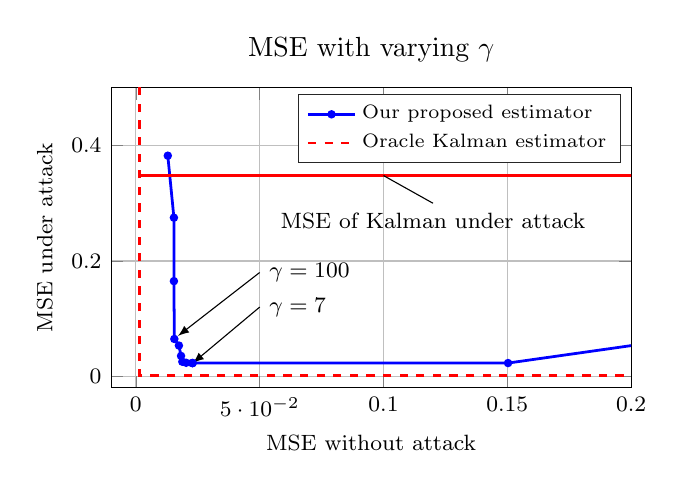
\begin{tikzpicture}
\begin{axis}
[	width=2.6in,
	height=1.5in,
	at={(0in,0in)},
	scale only axis,
	xmin=-0.01,
	xmax=0.2,
	ymin=-0.02,
	ymax=0.5,
	title={MSE with varying $\gamma$},
	xlabel={\footnotesize MSE without attack},
	ylabel={\footnotesize MSE under attack},
%	x label style={at={(axis description cs:0.5,-0.08)},anchor=north},
%	y label style={at={(axis description cs:-0.11,.5)},anchor=south},
	xticklabel style = {font=\footnotesize},
	yticklabel style = {font=\footnotesize},
	axis background/.style={fill=white},
	xmajorgrids,
	ymajorgrids,
	legend style={at={(0.98,0.98)}, anchor=north east, legend cell align=left, align=left, draw=white!15!black, font=\scriptsize}]
	
	 \addplot [color={blue}, line width=1pt, mark=*, mark size=1pt]
	table[row sep={\\}]
	{
%		2.73294  2.18893 \\ % gamma=0.1
%		2.7611  2.2588  \\  % gamma=0.2
%		2.73456  2.14272 \\ % gamma=0.5
%		2.70273  2.23093 \\ % gamma=1
%		2.5806  2.13751 \\  % gamma=2
%		 1.3291898141799852 \\ % gamma=4
		0.49171288806410334  0.23058873634922077 \\ % gamma=5
		0.15031158033658748 0.023028041755303673 \\% gamma=6
		0.022956004079827286  0.023069623748774245 \\ % gamma=7
		0.022892999120518853  0.02302036422425081 \\ % gamma=8
		0.022738740120155414  0.023028041755303673 \\ % gamma=10
		0.02031379510833805 0.023522751164769238 \\ % gamma=20
		0.018767389239823917 0.025297232039458894   \\ % gamma=30
		0.018239965010654734 0.03540481351322025 \\ % gamma=40
		0.017382121611668622 0.053386825865487555\\ % gamma=50
		0.015534591302800367 0.06477553708429706\\ % gamma=100
		0.015363288434118163 0.16504007534811177\\ % gamma=200
		0.015363288434118163 0.27504007534811177\\ % gamma=500
		0.012899244187193867 0.382451394009979\\ % gamma=1000
	} 
	;\addlegendentry{Our proposed estimator}
	
	
	
	 \addplot [dashed, color={red}, line width=1pt]
	table[row sep={\\}]
	{
	 3  0.0016205180878490848  \\
	 0.0016205180878490848  0.0016205180878490848 \\
	 0.0016205180878490848  30\\
	}
	;\addlegendentry{Oracle Kalman estimator}
	
	 \addplot [color={red}, line width=1pt]
	table[row sep={\\}]
	{
		0.002  0.3483651642262539\\
		3  0.3483651642262539\\
	}
	;%\addlegendentry{Kalman estimator}
	
	\draw[latex-] (0.017, 0.07)--(0.05,0.18) node[right]{\footnotesize  $\gamma=100$};
	\draw[latex-] (0.023, 0.023)--(0.05,0.12) node[right]{\footnotesize $\gamma=7$};
	\draw[latex-] (0.1, 2.5)--(2.3,5) node[right]{\footnotesize $\gamma=5$};
	\draw[-] (0.1, 0.348)--(0.12,0.3) node[below]{\footnotesize MSE of Kalman under attack};
	
   
\end{axis}

%\begin{axis}
%	[width=2.6in,
%	height=1.5in,
%	at={(3.5in,0in)},
%	scale only axis,
%	xmin=0,
%	xmax=2.1,
%	ymin=-0.1,
%	ymax=1.5,
%	title={MSE with varying attack magnitude},
%	xlabel={\footnotesize attack magnitude $||a||_\ift$},
%	ylabel={\footnotesize MSE under attack},
%	%	x label style={at={(axis description cs:0.5,-0.08)},anchor=north},
%	y label style={at={(axis description cs:-0.11,.5)},anchor=south},
%	xticklabel style = {font=\footnotesize},
%	yticklabel style = {font=\footnotesize},
%	axis background/.style={fill=white},
%	xmajorgrids,
%	ymajorgrids,
%	legend style={at={(0.02,0.98)}, anchor=north west, legend cell align=left, align=left, draw=white!15!black, font=\scriptsize}]
%	
%	
%	
%		\addplot [color={blue}, line width=1pt, mark=*, mark size=1pt]
%		table[row sep={\\}]
%		{   
%			0.1 0.02273998743284275\\
%			0.2 0.02309437925527503\\
%			0.5 0.022727416340979578\\
%			1 0.023028041755303673\\
%			1.5 0.04150262265679778\\
%			2  0.06361155341192473\\
%		}
%		;\addlegendentry{Our proposed estimator}
%		
%		\addplot [color={red}, line width=1pt, mark=*, mark size=1pt]
%		table[row sep={\\}]
%		{   
%			0.1 0.005836883178707939\\
%			0.2 0.016944741009078466 \\
%			0.5 0.09868982450677061 \\
%			1   0.3483651642262539\\
%			1.5 0.7777564157424298\\
%			2 1.394430537838036 \\
%		}
%		;\addlegendentry{Kalman estimator}
%	
%	
%	
%	
%	\draw[latex-] (0.2,24)--(0.4,31) node[right]{\footnotesize $\gamma=100$};
%	\draw[latex-] (0.42,13.4)--(1,13) node[right]{\footnotesize $\gamma=30$};
%	\draw[latex-] (2,8)--(2.4,10) node[right]{\footnotesize $\gamma=5$};
%	\draw[-] (1.4, 17.6)--(1.6,21) node[above]{\footnotesize MSE of Kalman under attack};
%	
%\end{axis}




\end{tikzpicture}





		\caption{Estimation mean square error (MSE) with varying tuning parameter $\gamma$. The attack magnitude is $\|a\|_\ift=1$.  } \label{fig:MSE_gamma}
	\end{subfigure}
\hspace{5pt}
	\begin{subfigure}{.48\textwidth}
		\centering
		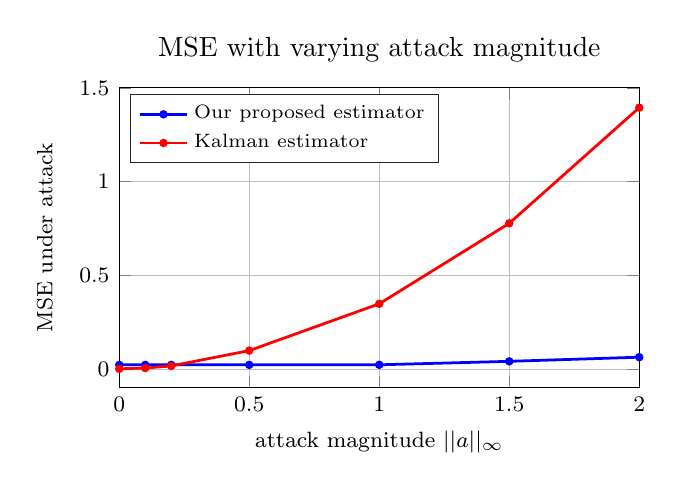
\begin{tikzpicture}
%\begin{axis}
%[	width=2.6in,
%	height=1.5in,
%	at={(0in,0in)},
%	scale only axis,
%	xmin=-0.01,
%	xmax=0.2,
%	ymin=-0.02,
%	ymax=0.5,
%	title={MSE with varying $\gamma$},
%	xlabel={\footnotesize MSE without attack},
%	ylabel={\footnotesize MSE under attack},
%%	x label style={at={(axis description cs:0.5,-0.08)},anchor=north},
%%	y label style={at={(axis description cs:-0.11,.5)},anchor=south},
%	xticklabel style = {font=\footnotesize},
%	yticklabel style = {font=\footnotesize},
%	axis background/.style={fill=white},
%	xmajorgrids,
%	ymajorgrids,
%	legend style={at={(0.98,0.98)}, anchor=north east, legend cell align=left, align=left, draw=white!15!black, font=\scriptsize}]
%	
%	 \addplot [color={blue}, line width=1pt, mark=*, mark size=1pt]
%	table[row sep={\\}]
%	{
%%		2.73294  2.18893 \\ % gamma=0.1
%%		2.7611  2.2588  \\  % gamma=0.2
%%		2.73456  2.14272 \\ % gamma=0.5
%%		2.70273  2.23093 \\ % gamma=1
%%		2.5806  2.13751 \\  % gamma=2
%%		 1.3291898141799852 \\ % gamma=4
%		0.49171288806410334  0.23058873634922077 \\ % gamma=5
%		0.15031158033658748 0.023028041755303673 \\% gamma=6
%		0.022956004079827286  0.023069623748774245 \\ % gamma=7
%		0.022892999120518853  0.02302036422425081 \\ % gamma=8
%		0.022738740120155414  0.023028041755303673 \\ % gamma=10
%		0.02031379510833805 0.023522751164769238 \\ % gamma=20
%		0.018767389239823917 0.025297232039458894   \\ % gamma=30
%		0.018239965010654734 0.03540481351322025 \\ % gamma=40
%		0.017382121611668622 0.053386825865487555\\ % gamma=50
%		0.015534591302800367 0.06477553708429706\\ % gamma=100
%		0.015363288434118163 0.16504007534811177\\ % gamma=200
%		0.015363288434118163 0.27504007534811177\\ % gamma=500
%		0.012899244187193867 0.382451394009979\\ % gamma=1000
%	} 
%	;\addlegendentry{Our proposed estimator}
%	
%	
%	
%	 \addplot [dashed, color={red}, line width=1pt]
%	table[row sep={\\}]
%	{
%	 3  0.0016205180878490848  \\
%	 0.0016205180878490848  0.0016205180878490848 \\
%	 0.0016205180878490848  30\\
%	}
%	;\addlegendentry{Oracle Kalman estimator}
%	
%	 \addplot [color={red}, line width=1pt]
%	table[row sep={\\}]
%	{
%		0.002  0.3483651642262539\\
%		3  0.3483651642262539\\
%	}
%	;%\addlegendentry{Kalman estimator}
%	
%	\draw[latex-] (0.017, 0.07)--(0.05,0.18) node[right]{\footnotesize  $\gamma=100$};
%	\draw[latex-] (0.023, 0.023)--(0.05,0.12) node[right]{\footnotesize $\gamma=7$};
%	\draw[latex-] (0.1, 2.5)--(2.3,5) node[right]{\footnotesize $\gamma=5$};
%	\draw[-] (0.1, 0.348)--(0.12,0.3) node[below]{\footnotesize MSE of Kalman under attack};
%	
%   
%\end{axis}

\begin{axis}
	[width=2.6in,
	height=1.5in,
	at={(3.5in,0in)},
	scale only axis,
	xmin=0,
	xmax=2.0,
	ymin=-0.1,
	ymax=1.5,
	title={MSE with varying attack magnitude},
	xlabel={\footnotesize attack magnitude $||a||_\ift$},
	ylabel={\footnotesize MSE under attack},
	%	x label style={at={(axis description cs:0.5,-0.08)},anchor=north},
	y label style={at={(axis description cs:-0.11,.5)},anchor=south},
	xticklabel style = {font=\footnotesize},
	yticklabel style = {font=\footnotesize},
	axis background/.style={fill=white},
	xmajorgrids,
	ymajorgrids,
	legend style={at={(0.02,0.98)}, anchor=north west, legend cell align=left, align=left, draw=white!15!black, font=\scriptsize}]
	
	
	
		\addplot [color={blue}, line width=1pt, mark=*, mark size=1pt]
		table[row sep={\\}]
		{   0 0.022738740120155414\\
			0.1 0.02273998743284275\\
			0.2 0.02309437925527503\\
			0.5 0.022727416340979578\\
			1 0.023028041755303673\\
			1.5 0.04150262265679778\\
			2  0.06361155341192473\\
		}
		;\addlegendentry{Our proposed estimator}
		
		\addplot [color={red}, line width=1pt, mark=*, mark size=1pt]
		table[row sep={\\}]
		{   0 0.0016205180878490848\\
			0.1 0.005836883178707939\\
			0.2 0.016944741009078466 \\
			0.5 0.09868982450677061 \\
			1   0.3483651642262539\\
			1.5 0.7777564157424298\\
			2 1.394430537838036 \\
		}
		;\addlegendentry{Kalman estimator}
	
	
	
	
	\draw[latex-] (0.2,24)--(0.4,31) node[right]{\footnotesize $\gamma=100$};
	\draw[latex-] (0.42,13.4)--(1,13) node[right]{\footnotesize $\gamma=30$};
	\draw[latex-] (2,8)--(2.4,10) node[right]{\footnotesize $\gamma=5$};
	\draw[-] (1.4, 17.6)--(1.6,21) node[above]{\footnotesize MSE of Kalman under attack};
	
\end{axis}




\end{tikzpicture}





		\caption{Estimation mean square error (MSE) with varying attack magnitude. The parameter $\gamma$ is set as $\gamma=10$. } \label{fig:MSE_mag}
	\end{subfigure}
	\caption{}
	\label{fig:MSE}
\end{figure}



%The estimation mean square error (MSE) in the absence and in the presence of attack is presented in Table \ref{tab:MSE}.
%The initial state is set to be $x(0)=\mathbf{0}$. When sensor 1 is under manipulation, the bias data is a random value uniformly distributed on interval $(-10,10)$. When sensor 4 is under manipulation, the bias data is a random value uniformly distributed on interval $(-\pi,\pi)$. The MSE of our proposed estimator is approximately the same as that of Kalman estimator in the absence of attack. In the presence of attack, the MSE of our proposed estimator is smaller.
%
%\begin{table}[h]
%	\caption{Mean square error of two estimators}\label{tab:MSE}
%	\begin{tabular}{c|c|c|c}
%	\hline 
%		Estimator & \makecell[c]{\small MSE without\\ attack} & \makecell[c]{\small MSE when \\ $\Ic=\{1\}$} &\makecell[c]{\small MSE when \\ $\Ic=\{4\}$} \\
%	\hline 
%		\makecell[c]{Kalman\\ estimator} & 0.0121 & 0.6652 & 2.8834 \\ 
%		\hline
%		\makecell[c]{Our proposed\\ estimator}  & 0.0122 & 0.4927 & 0.5025 \\
%		\hline 
%	\end{tabular}
%\end{table}





\section{Conclusion}\label{sec:conclusion}
This paper considers LTI system with Gaussian noise against sparse integrity attack on a subset of sensors. 
Under the geometric multiplicity assumption on stable eigenvalues of $A$, we propose an estimation scheme that is secure to $(p,m)$-sparse attack as long as the system is $2p$-sparse detectable. 
To achieve this, we prove that the span of the rows of $G^\Uc_i$ is equivalent to the observable space corresponding to unstable states, based on which the canonical form $H_i$ is designed. The proposed estimator is formulated as a convex optimization problem based on $H_i$, where by careful design, the estimation of stable states is always secured. 
Moreover, in the absence of attack, the proposed estimation coincides with Kalman estimation for certain probability, which can be adjusted by tuning parameter $\gamma$ to balance between the performance with and without attack.
We further prove that the $2p$-sparse detectable is necessary for secure estimation, which means our proposed estimator achieves this fundamental limit with good performance in the absence of attack and low computation complexity.
%For general $A$ without the geometric multiplicity assumption, calculating sparse observability index is NP-hard. 

%In previous works, we proposed a information fusion scheme by decomposing Kalman estimation into the linear combination of local estimates. 
%However, whether this estimator is resilient cannot be validated within polynomial time.
%In this paper, by introducing the assumption that all the eigenvalues of $A$ have geometric multiplicity 1, we prove that the structure of matrix $G_i$ is closely related to observability matrix of system $(A,C_i)$. This result enables us to design a secure estimator that is resilient to $p$ compromised sensors as long as the system is $2p$-sparse observable and this can be further relaxed to $2p$-sparse detectable. Moreover, the estimate coincides to Kalman estimate for certain probability in the absence of attack.  we design an algorithm that can compute sparse observability index in polynomial time. 
%However, when the geometric multiplicity is greater than 1, Lemma \ref{lm:span} no long holds and there are instances where $\rs(G_i)\neq \rs{O_i}$. We are currently investigating the solution in this case. Nevertheless, by decomposing the $n$ dimensional space into multiple orthogonal generalized eigenspaces, the problem of checking sparse observability can be significantly simplified. 


%%%%%%%%%%%%%%%%%%%%%%%%%%%%%%%%%%%%%%%%%%%%%%%%%%%%%%%%%%%%%%%%%%%%%%%%%%%%%%%%
{\LARGE \bf \centering Appendix}
\appendix
\section{Proof of Theorem \ref{th:span}}\label{ap:span}
\begin{proof}
	Define the characteristic polynomial of $A$ as $p(x)=a_n x^n +\cdots+a_1 x +a_0$.
Define polynomial fraction  $q_\pi(x)$ with respect to constant $\pi$ as
$q_\pi(x)=\frac{p(x)-p(\pi)}{x-\pi}$ where $x\neq \pi$.
Therefore,
$$q_\pi(A)(A-\pi I) = p(A)-p(\pi)I=-p(\pi)I ,$$
where the last equality comes from Cayley-Hamilton Theorem.
As a result, when $\pi$ is not the eigenvalue of $A$, we have
\begin{align}\label{A-lambdaI}
(A-\pi I)^{-1}=-\frac{1}{p(\pi)} q_\pi(A).
\end{align}
In order to simplify notations, we define 
\begin{equation}\label{eq:bjk}
b_{j,k}\triangleq-\frac{1}{p(\pi_j)}\sum_{i=0}^{n-k-1} a_{i+k+1} \pi_j^i,
\end{equation}
where $\pi_j$ is the $j$-th diagonal element of $\Pi$, i.e., $j$-th eigenvalue of $A-KCA$ as defined in \eqref{eq:VLambda}.
According to (\ref{A-lambdaI}), the $j$-th row of matrix $G_i$ can be reformulated as
$$C_{i} A\left(A-\pi_{j} I\right)^{-1}=
\begin{bmatrix}
b_{j,0} & b_{j,1} & \cdots  & b_{j,n-1} 
\end{bmatrix} O_i A.$$
Therefore, $G_i$ can be interpreted as follows
\begin{align*}
G_i = \begin{bmatrix}
b_{1,0} & b_{1,1} & \cdots  & b_{1,n-1} \\
b_{2,0} & b_{2,1} & \cdots  & b_{2,n-1} \\
\vdots & \vdots & \ddots  & \vdots \\
b_{n,0} & b_{n,1} & \cdots  & b_{n,n-1} 
\end{bmatrix}
O_i A 
= & \mathcal{D}_1\mathcal{D}_2\mathcal{D}_3 O_i A , %\label{eq:GandOA}		
\end{align*}
where $\mathcal{D}_1\triangleq\text{diag}\left(-\frac{1}{p(\pi_1)},-\frac{1}{p(\pi_2)},\cdots,-\frac{1}{p(\pi_n)}\right)$,
\begin{align*}
\mathcal{D}_2\triangleq
\begin{bmatrix}
\pi_1^{n-1} & \pi_1^{n-2} & \cdots  & 1 \\
\pi_2^{n-1} & \pi_2^{n-2} & \cdots  & 1 \\
\vdots & \vdots & \cdots  & \vdots \\
\pi_n^{n-1} & \pi_n^{n-2} & \cdots  & 1
\end{bmatrix}, 
\mathcal{D}_3\triangleq
\begin{bmatrix}
a_n & 0 & \cdots &   0 \\
a_{n-1} & a_n & \cdots &   0 \\
\vdots & \vdots & \ddots  & \vdots \\
a_1 & a_2 & \cdots  & a_n 
\end{bmatrix}.
\end{align*}
According to Assumption \ref{as:distinct_eigvalue}, all $\pi_j$ are distinct eigenvalues and they are not the eigenvalues of $A$, i.e. the diagonal matrix $\mathcal{D}_1$ and the Vandermonde matrix $\mathcal{D}_2$ are invertible. Moreover, $a_n=1$. Therefore, the lower triangular Toeplitz matrix $\mathcal{D}_3$ is invertible and thus $\rs(G_i)=\rs(O_i A)$. 		
We continue to prove $\rs(O_i)=\rs(O_i A)$. Considering that $A^n=-a_{n-1}A^{n-1}-\cdots-a_0 I$, one obtains the following equation \eqref{eq:O_OA}.
\begin{equation}
\label{eq:O_OA}
O_i A=
\begin{bmatrix}
0 & 1 & 0 &  \cdots & 0 \\
0 & 0 & 1 &  \cdots & 0 \\
\vdots & \vdots & \vdots & \ddots & \vdots \\
0 & 0 & 0 &  \cdots & 1 \\
-a_0 & -a_1 & -a_2 & \cdots &  -a_{n-1}
\end{bmatrix}
O_i .
\end{equation}	%\vspace{-20pt}
According to Assumption \ref{as:distinct_eigvalue}, $A$ is invertible and $a_0=(-1)^n\det(A)\neq 0$, which leads to the equation that $\rs(O_i)=\rs(O_i A)$.
As a result, $\rs(G_i^\Uc)$=$\rs(O_i^\Uc)$. We continue to prove that $\rs(O_i^\Uc)=\rs(H_i^\Uc).$
Since $A_1$ is assumed to be in the Jordan canonical form and all eigenvalues have geometric multiplicity 1, one can verify that nonzero columns of $O^\Uc_i$ are linear independent. Therefore, $i\in\Ec_j$ is equivalent to that $j$-th column of $O_i$ is non-zero, i.e., $O^\Uc_i$ has the same row-span with the canonical form $H^\Uc_i$.
$\square$
\end{proof}

%\section{Proof of Theorem \ref{th:att_obs}}\label{ap:att_obs}
%
%\begin{proof}[Proof of Theorem \ref{th:att_obs}]
%	In view of Theorem \ref{th:TAC} and Lemma \ref{lm:least_square}, it suffices to prove that the following two propositions are equivalent:
%	\begin{enumerate}
%		\item The system is $2p$-sparse observable.
%		\item The following inequality holds for all $x \neq \mathbf{0}$, $x\in\Rb^n$:
%		\begin{equation}\label{eq:proof_cond}
%		\sum_{i \in \mathcal{I}}\left\|H_{i} x\right\|_{1}<\sum_{i \in \mathcal{I}^{c}}\left\|H_{i} x\right\|_{1}, \quad \forall\ \Ic\subset \Oc, |\mathcal{I}|\leq p .
%		\end{equation}
%	\end{enumerate}
%	Based on the form of $H_i$ in Theorem \ref{th:span}, inequality \eqref{eq:proof_cond} can be written as 
%	\begin{equation*}
%	\sum_{j=1}^{n} \sum_{i \in \mathcal{I}\cap\Ec_j}|x_j|<\sum_{j=1}^{n} \sum_{i \in \mathcal{I}^c\cap\Ec_j}|x_j| 
%	\end{equation*}
%	or equivalently 
%	$$
%	\sum_{j=1}^{n} c_j(\Ic)\cdot|x_j|<\sum_{j=1}^{n} h_j(\Ic)\cdot|x_j| .
%	$$
%	If the system is $2p$-sparse observable, we have $c_j(\Ic)<h_j(\Ic)$ for all $j\in\{1,2,\cdots,n\}$. Thus, $\sum_{j=1}^{n} \left(h_j(\Ic)-c_j(\Ic)\right)\cdot|x_j| >0$ holds for all $x\neq \mathbf{0}$.
%	If the system is not $2p$-sparse observable, there exists $\Ic^*$ with $|\Ic^*|=p$ and $j^*$ such that $c_{j^*}(\Ic^*)>h_{j^*}(\Ic^*)$. One can design $x\neq \mathbf{0}$ such that 
%	$$\left(c_{j^*}(\Ic^*)-h_{j^*}(\Ic^*)\right)\cdot|x_{j^*}|> \sum_{j\neq j^*}\left(h_{j}(\Ic^*)-c_{j}(\Ic^*)\right)\cdot|x_j| .$$
%	Therefore, condition \eqref{eq:proof_cond} is violated and the proof is completed. $\square$
%\end{proof}

\section{Proof of Theorem \ref{th:no_attack}}\label{ap:ap_no_attack}
\begin{proof}[Proof of Theorem \ref{th:no_attack}]
	
	Considering the KKT condition of problem \eqref{pb:resilient_LASSO}, one obtains that if 
	$$\left\|\Wc \begin{bmatrix}
	\mu(k) \\
	\Nc H \tilde{x}(k)
	\end{bmatrix}\right\|_\ift\leq\gamma,$$ then the solution $\nu(k)$ satisfy that $\nu(k)=\mathbf{0}$. In this scenario, solutions to problem \eqref{pb:resilient_LASSO} and problem \eqref{pb:least_square} are equivalent and the solution $\tilde{x}(k),\mu(k),\nu(k)$ satisfy
	\begin{equation}\label{eq:lasso_recover}
	\tilde{x}(k)=\tilde{x}_\ls(k)=\hat{x}(k),\ \mu(k)=\varphi(k),\ \nu(k)=\mathbf{0}.
	\end{equation}
	According to Lemma \ref{lm:least_square}, the solution $\varphi(k)$ of problem \eqref{pb:least_square} satisfy the following equation:
	\begin{equation}\label{eq:ls_recover}
	\tilde{x}_\ls(k)=\hat{x}(k),\ \varphi(k)=(I-GF)\epsilon(k),
	\end{equation}
	where $\hat{x}(k)$ is the fixed gain Kalman estimation defined in \eqref{eq:fix_gain_kalman}.
	Combining \eqref{eq:ls_recover} and \eqref{eq:lasso_recover}, result in Theorem \ref{th:no_attack} is obtained. $\square$
\end{proof}

\section{Proof of Theorem \ref{th:main}}\label{ap:main}
Before proving Theorem \ref{th:main}, we need the following Lemma.
Define the number of honest sensors and compromised sensors (w.r.t. compromised set $\Ic$) that can observe state $j$ as:
\begin{align*}
h_j(\Ic)\triangleq |\Ec_j\cap \Ic^c|, \
c_j(\Ic)\triangleq |\Ec_j\cap \Ic|.
\end{align*}
We have the following lemma quantifying the property of $h_j(\Ic)$ and $c_j(\Ic)$.  
\begin{lemma}\label{lm:cj<hj}
	The following two propositions are equivalent.
	\begin{enumerate}
		\item The system is $2p$-sparse observable.
		\item For any $\Ic$ with $|\Ic|=p$, the inequality $c_j(\Ic)<h_j(\Ic)$ holds for all $j\in\{1,2,\cdots,n\}$.
	\end{enumerate}
\end{lemma}
\begin{proof}[Proof of Lemma \ref{lm:cj<hj}]
	We prove the contrapositive of (1)$\Rightarrow$(2). Supposing that there exists $j^*$ and $\Ic^*$ with $|\Ic^*|=p$ such that $ c_{j^*}(\Ic^*)\geq h_{j^*}(\Ic^*)$, then
	$h_{j^*}(\Ic^*)\leq c_{j^*}(\Ic^*)\leq |\Ic^*|=p$. Noticing that $c_j(\Ic)+h_j(\Ic)=|\Ec_j|$ holds for all $\Ic$, we have $|\Ec_{j^*}|\leq 2p$. 
	There exists set $\Ac$ that satisfy $\Ac\supseteq\Ec_{j^*}$ and $|\Ac|=2p$.
	According to the definition of $\Ec_{j^*}$, there exists no sensor in set $\Oc\setminus \Ac$ who can observe state $j^*$, i.e.,
	\begin{equation*}
	e_{j^*}\notin \rs(O_i),\ \forall i\in\Oc\setminus \Ac.
	\end{equation*}
	As a result, system $(A,C_{\Oc\setminus\Ac})$ is not $2p$-sparse observable according to Definition \ref{df:sparse_obs}. 
	
	We proceed to prove (2)$\Rightarrow$(1). 
	Since for any $\Ic$ with $|\Ic|=p$, $h_j(\Ic)>c_j(\Ic)\geq 0$, the system sparse observability index is at least $p$. Therefore, for each $j\in\{1,2,\cdots,n\}$, there exists an $\Ic^*$ such that $c_j(\Ic^*)=p$, and thus $|\Ec_j|=h_j(\Ic^*)+c_j(\Ic^*)\geq 2p+1$. According to the definition $\Ec_j$, there are at least $2p+1$ sensors that can observe sensor $j$, and the system is $2p$-sparse observable.	
	$\square$
\end{proof}

We need the following notations for the proof.
Define the unstable part and stable parts of $x$ as the following where $x_u\in\Cb^{n_u\times 1}$ and $x_s\in\Cb^{n_s\times 1}$. Similarly, divide matrix $H_i$ into four parts based on Theorem \ref{th:span} where $H_{uu,i}\in\Cb^{n_u\times n_u}$ and $H_{ss,i}\in\Cb^{n_s\times n_s}$.
\begin{align*}
x = 
\left[
\begin{array}{c}
x_u\\x_s
\end{array}
\right],\
%\begin{array}{l}
%\hspace{-6pt}\left. \right\} \text{first $n_u$ entries}\\
%\hspace{-6pt}\left. \right\} \text{last $n_s$ entries}
%\end{array} .\\
	H_i=\begin{bmatrix}
H_{uu,i}	& 	H_{us,i} \\
\mathbf{0}_{n_s\times n_u} & H_{ss,i}
\end{bmatrix} .
\end{align*}
Define $\eta_{i}\triangleq P_i\zeta_{i}$.
Similar to $x$, $\tilde{x}$ and $\eta_i$ are also divided to $\tilde{x}_u,\tilde{x}_s,\eta_{i,u},\eta_{i,s}$ in the same way.

	\begin{proof}[Proof of Theorem \ref{th:main}]
	Consider the KKT condition of problem (\ref{pb:resilient_LASSO}) and denote the dual variables for equation constraints as $\lambda=[\lambda_1{'},\cdots,\lambda_m{'}]{'}\in \Cb^{mn\times 1}$:	
	\begin{align}
	(\tilde{M}^{-1}+\Nc{'}\Nc)\mu+\Nc{'} \Nc H\tilde{x} - \lambda &= \mathbf{0}, \label{eq:KKT1}\\
	H{'} \Nc{'}\Nc\mu+H{'} \Nc{'} \Nc H\tilde{x} -  H{'}\lambda &= \mathbf{0}, \label{eq:KKT2} \\
	\gamma \cdot  \tilde{\nu} - \lambda &= \mathbf{0}, \label{eq:KKT3} \\
	{Y} - H \tilde{x} - \mu - \nu &= \mathbf{0},  \label{eq:KKT4}
	\end{align}
	where $\tilde{\nu}$ belongs to the subgradient of $\|\nu\|_1$, i.e., for the $i$-th entry:
	\begin{align*}
	\begin{cases}
	[\tilde{\nu}]_i=-1 ,& \ [\nu]_i<0 \\
	[\tilde{\nu}]_i=1 , &\ [\nu]_i>0  \\
	[\tilde{\nu}]_i\in\left[-1,1\right],& \ [\nu]_i=0 
	\end{cases}.
	\end{align*}
	
	Combining (\ref{eq:KKT1}) and (\ref{eq:KKT2}) leads to:
	\begin{equation}\label{eq:KKT12}
	\begin{bmatrix}
	\tilde{M}^{-1}+\Nc{'}\Nc & \Nc{'} \Nc H\\
	H{'} \Nc{'} \Nc  & H{'} \Nc{'} \Nc H
	\end{bmatrix}
	\begin{bmatrix}
	\mu \\ \tilde{x}
	\end{bmatrix}=
	\begin{bmatrix}
	\lambda \\ H{'} \lambda 
	\end{bmatrix}.
	\end{equation}
	According to the definition of $\Nc$, the first $n_u$ rows of $H{'} \Nc{'} \Nc$ are zeros. Therefore, we extract the non-zeros part of equation (\ref{eq:KKT12}) in the following:
	\begin{equation}\label{eq:KKT12_nonzero}
	\begin{bmatrix}
	\tilde{M}^{-1}+\Nc{'}\Nc & \Nc{'} \Nc H \Lc{'}\\
	\Lc H{'} \Nc{'} \Nc  &  \Lc H{'} \Nc{'} \Nc H \Lc{'}
	\end{bmatrix}
	\begin{bmatrix}
	\mu \\ \tilde{x}_s
	\end{bmatrix}=
	\begin{bmatrix}
	\lambda \\ \Lc H{'} \lambda 
	\end{bmatrix}.
	\end{equation}
	where $\Lc\triangleq 
	\begin{bmatrix}
	\mathbf{0}_{n_s\times n_u} & I_{n_s}
	\end{bmatrix}.
	$
	%Notice that
	%\begin{align}
	%&\Lc H{'} \Nc{'} \Nc H \Lc{'} 
	%- \Lc H{'} \Nc{'} \Nc(\tilde{M}^{-1}+\Nc{'}\Nc)^{-1} \Nc{'} \Nc H \Lc{'} \notag \\
	%= &\Lc H{'} \Nc{'}  \left(I -\Nc(\tilde{M}^{-1}+\Nc{'}\Nc)^{-1}\Nc{'} \right)  \Nc H \Lc{'} . \label{eq:schur_comp}
	%\end{align}
	%Since I−\Nc(M~−1+\Nc⊤\Nc)−1\Nc⊤ is invertible and \LcH⊤\Nc⊤ is row full-rank (???) is also invertible due to the Frobenius rank inequality.
	%Therefore, according to the result of Schur complement, matrix on the left of (???) is invertible.
	Rewrite (\ref{eq:KKT12_nonzero}) as:
	\begin{align}\label{eq:KKT12_matrix}
	\left(
	\begin{bmatrix}
	I_{mn} & \mathbf{0} \\
	\mathbf{0}  &  \Lc H{'} \Nc{'}
	\end{bmatrix}
	\Wc
	\begin{bmatrix}
	I_{mn} & \mathbf{0} \\
	\mathbf{0}  &  \Nc H \Lc{'}
	\end{bmatrix}
	\right)
	\begin{bmatrix}
	\mu \\ \tilde{x}_s
	\end{bmatrix}=
	\begin{bmatrix}
	I_{mn} & \mathbf{0} \\
	\mathbf{0}  &  \Lc H{'}
	\end{bmatrix}
	\lambda .
	\end{align}
	Notice that $\Wc$ is positive definite and $\begin{bmatrix}
	I_{mn} & \mathbf{0} \\
	\mathbf{0}  &  \Lc H{'} \Nc{'}
	\end{bmatrix}$
	is full row-rank,
%	\footnote{
%		$\Lc H{'} \Nc{'}=
%		\begin{bmatrix}
%		H{'}_{ss,1} & H{'}_{ss,2} & \cdots & H{'}_{ss,m} % !!!NOtice that H_{ss,i}=G_{ss,i}, if this matrix not full row fank, then $G{'}_{ss,1} & G{'}_{ss,2}$ is row rank defected and there are unobservable stable states.
%		\end{bmatrix}
%		$ is row full-rank due to the fact that for every stable state, there is at least one sensor who is able to observe the state.
%	}, 
	due to the Frobenius rank inequality, the matrix on the left of (\ref{eq:KKT12_matrix}) is also invertible, and thus the following matrix is well-defined:
	\begin{align}\label{eq:def_H}
	\Fc	\triangleq
	\left(
	\begin{bmatrix}
	I_{mn} & \mathbf{0} \\
	\mathbf{0}  &  \Lc H{'} \Nc{'}
	\end{bmatrix}
	\Wc
	\begin{bmatrix}
	I_{mn} & \mathbf{0} \\
	\mathbf{0}  &  \Nc H \Lc{'}
	\end{bmatrix}
	\right)^{-1}
	\begin{bmatrix}
	I_{mn} & \mathbf{0} \\ \mathbf{0} &\Lc H{'}
	\end{bmatrix}.
	\end{align}
	
	%Sufficient condition of (???) is:
	%\begin{align}\label{eq:KKT2_2}
	%	\Nc \mu + \Nc H \tilde{x} - \frac{1}{2}(\Nc^\dag){'} \lambda = \mathbf{0} 
	%\end{align}
	%where \Nc\dag is the pseudo-inverse of \Nc.
	%Combining (???) and (???) leads to:
	%\begin{equation}\label{eq:KKT12}
	%	\begin{bmatrix}
	%		\tilde{M}^{-1}+\Nc{'}\Nc & \Nc{'} \\
	%		\Nc & I
	%	\end{bmatrix}
	%	\begin{bmatrix}
	%		\mu \\ \Nc H \tilde{x}
	%	\end{bmatrix}=\frac{1}{2}
	%	\begin{bmatrix}
	%		\lambda \\ (\Nc^\dag){'} \lambda 
	%	\end{bmatrix}.
	%\end{equation}
	
	According to (\ref{eq:KKT3}), $\|\lambda\|_\infty \leq \gamma$. 
	Therefore we have the following from (\ref{eq:KKT12_matrix})
	\begin{equation}\label{eq:mu_xs_bounded}
	\left\|\begin{bmatrix}
	\mu \\ \tilde{x}_s 
	\end{bmatrix}\right\|_\infty
	\leq \gamma \cdot
	\left\|\Fc\right\|_\infty.
	\end{equation}
	
	Now we continue to prove that the estimation of unstable states $\tilde{x}_u$ are resilient.
	Rewrite the optimization problem \eqref{pb:resilient_LASSO} as 
	\begin{align*}
	\underset{{\tilde{x}},\ \mu}{\text{minimize}}&\quad \frac{1}{2} 
	\begin{bmatrix}
	\mu \\
	\Nc H \tilde{x}
	\end{bmatrix}^{'} \Wc
	\begin{bmatrix}
	\mu \\
	\Nc H \tilde{x}
	\end{bmatrix} + \gamma\left\|{Y}-\mu-H \tilde{x}\right\|_1 
	\end{align*}
	where the time index is omitted for notation simplicity.
	Consider the 1-norm term in the objective function:
	\begin{align*}
	&\left\| {Y}-\mu-H \tilde{x} \right\|_1
	=\sum_{i=1}^{m} 
	\left\|\eta_{i,u}-\mu_{i,u}-(H_{uu,i} \tilde{x}_u + H_{us,i} \tilde{x}_s) \right\|_1 
	+ \sum_{i=1}^{m} \left\|\eta_{i,s}-\mu_{i,s}- H_{ss,i} \tilde{x}_s \right\|_1 
	\end{align*}
	where $\eta_{i,u}, \mu_{i,u}$ is the vector composed of first $n_u$ element of $\eta_{i}, \mu_{i}$ and 
	$\eta_{i,s}, \mu_{i,s}$ is the vector composed of last $n_s$ element of $\eta_{i}, \mu_{i}$.
	Suppose that $\mu$ and $\tilde{x}_s$ have taken the value of optimal solution $\mu^*, \tilde{x}_s^*$, it is sufficient to minimize the following :
	\begin{align}\label{pb:1-norm_min}
	\min_{\tilde{x}_u} \sum_{i=1}^{m} \left\|\eta_{i,u}-\mu^*_{i,u}- H_{us,i} \tilde{x}^*_s - H_{uu,i} \tilde{x}_u \right\|_1  .
	\end{align}
	Define $\xi_i\triangleq \eta_{i,u}-\mu^*_{i,u}- H_{us,i} \tilde{x}^*_s $ and recall $[\cdot]_j$ is the $j$-th entry of a vector. The objective function in (\ref{pb:1-norm_min}) can be written as 
	\begin{align}
	&\sum_{i=1}^{m}\sum_{j=1}^{n_u} \left| [\xi_i]_j -[H_{uu,i} \tilde{x}_u]_j \right| 
	=\sum_{j=1}^{n_u}\sum_{i\in\Ec_j} \left| [\xi_i]_j -\tilde{x}_j \right| . \label{eq:solve_for_median}
	\end{align}
	where $\Ec_j$ is the index set of sensors that can observe state $j$ that is defined in \eqref{eq:def_Ec}.
	For each unstable state $j\in\Uc$, the minimizer $\tilde{x}_j$ of objective (\ref{eq:solve_for_median}) could be explicitly written as the median of all $[\xi_i]_j$ among $i\in\Ec_j$.
	
	Before proving that $\tilde{x}_j$ is bounded, let us define the following operator: $f_{i}: R \times R \times \cdots \times R \rightarrow R,$ such that $f_{i}\left(\alpha_{l}, l\in\{1,\cdots,L\}\right)$ equals to the $i$-th smallest element in the set $\left\{\alpha_{1}, \ldots, \alpha_{L}\right\} .$ For even number $i$, we further define 
	$$f_{\frac{i+1}{2}} = \left(f_{\frac{i}{2}} + f_{\frac{i}{2}+1}\right)/2.$$ 
	Thus, $f_{(L+1)/2}\left(\alpha_{l}, l\in\{1,\cdots,L\}\right)$ is the median number of set $\left\{\alpha_{1}, \ldots, \alpha_{L}\right\}$ and the solution to problem \eqref{pb:1-norm_min} is 
	\begin{align*}
	\tilde{x}_j = f_{(|\Ec_j|+1)/2}\left([\xi_i]_j, i\in\Ec_j\right),j\in\Uc .
	\end{align*}
	Define the uncorrupted data corresponding to sensor $i$ as $\eta^o_{i}=P_i\zeta^o_i$. Define $\xi^o_{i}$ correspondingly as $\xi^o_i\triangleq \eta^o_{i,u}-\mu^*_{i,u}- H_{us,i} x^*_s $.
	Recalling that the number of honest sensors and compromised sensors that can observe unstable state $j\in\Uc$ are $h_j$ and $c_j$, we have
	\begin{align}	
	f_{(h_j-c_j)}\left([\xi^o_i]_j, i\in\Ec_j\right) &\leq
	f_{(m+1)/2}\left([\xi_i]_j, i\in\Ec_j\right), \label{eq:x_u_leftbound}\\
	f_{(m+1)/2}\left([\xi_i]_j, i\in\Ec_j\right)&\leq 
	f_{2c_j}\left([\xi^o_i]_j, i\in\Ec_j\right) .  \label{eq:x_u_rightbound}
	\end{align}\	According to Lemma \ref{lm:cj<hj}, $h_j-c_j>0$ and $2c_j<h_j+c_j=|\Ec_j|$.
	As a result, according to (\ref{eq:x_u_leftbound}) and (\ref{eq:x_u_rightbound}), one obtains
	\begin{align}\label{eq:med_bound}
	\min \left\{ [\xi^o_i]_j, i\in\Ec_j \right\}\leq \tilde{x}_j\leq \max \left\{ [\xi^o_i]_j, i\in\Ec_j \right\},\ j\in\Uc .
	\end{align}
	Consider the following optimization problem where observation are not influenced by attack:
	\begin{align*}
	\underset{{\tilde{x}}^o,\mu^o}{\text{minimize}}&\quad \frac{1}{2} 
	\begin{bmatrix}
	\mu^o \\
	\Nc H \tilde{x}^o
	\end{bmatrix}^{'} \Wc
	\begin{bmatrix}
	\mu^o \\
	\Nc H \tilde{x}^o
	\end{bmatrix} + \gamma^o\left\|{Y}^o-\mu^o-H \tilde{x}^o\right\|_1 ,
	\end{align*}
	where ${Y}^o$ is composed of $P_i\zeta_i^o$. Denote the solution to this problem as ${\tilde{x}}^o,\mu^o$.
	According to Theorem \ref{th:no_attack}, by choosing 
	$$\gamma^o=	\left\|\Wc \begin{bmatrix}
	\left(I-GF\right)\epsilon^o(k) \\
	\Nc H \hat{x}^o(k)
	\end{bmatrix}\right\|_\ift, $$
	the solution coincides with Kalman estimation, i.e., $\tilde{x}^o(k)=\hat{x}^o(k)$.
	Similar to previous analysis, the solution $\tilde{x}^o$ satisfies 
	\begin{align}\label{eq:normal_solution}
	[\tilde{x}^o]_j=f_{(|\Ec_j|+1)/2}\left( [P_i\zeta_{i}^o-\mu^o_i]_j, i\in\Ec_j \right), \forall j\in\Uc\cup \Sc.
	\end{align}
	Combining \eqref{eq:med_bound} and \eqref{eq:normal_solution} leads to that, for every $j\in\Uc$,
	\begin{align*}
	\left|[\tilde{x}]_j-[\tilde{x}^o]_j\right| =\left|[\tilde{x}]_j-[\hat{x}^o]_j\right|
	\leq &
	\max_{i_1,i_2\in \Ec_j} \left| \left[P_{i_1} \zeta^o_{i_1}(k)\right]_j- \left[P_{i_2} \zeta^o_{i_2}(k)\right]_j \right| 
	+ \|\mu^*\|_\infty+ \|\mu^o\|_\infty\\
	\leq& \max_{i_1,i_2\in \Ec_j} \left| \left[P_{i_1} \zeta^o_{i_1}(k)\right]_j- \left[P_{i_2} \zeta^o_{i_2}(k)\right]_j \right| +(\gamma+\gamma^o)\|\Fc\|_\ift.
	\end{align*}
	Recall that $P_i\epsilon_{i}(k)=P_i \zeta_i (k)-H_ix(k)$. Since for all $i_1,i_2\in \Ec_j$, one obtains $[H_{i_1}x(k)]_j=[x(k)]_j=[H_{i_2}x(k)]_j,\forall k\in\Zb^+$. Thus, we have
	\begin{align*}
	&\max_{i_1,i_2\in \Ec_j} \left| \left[P_{i_1} \zeta^o_{i_1}(k)\right]_j- \left[P_{i_2} \zeta^o_{i_2}(k)\right]_j \right| =\max_{i_1,i_2\in \Ec_j} \left| \left[P_{i_1} \epsilon^o_{i_1}(k)\right]_j- \left[P_{i_2} \epsilon^o_{i_2}(k)\right]_j \right| ,
	\end{align*}
	whose variance is uniformly bounded for all $k$ according to Lemma \ref{lm:epsilon}. Similarly, $\gamma^o$ is also uniformly bounded for all $k$. 
	Recalling that $\tilde{x}_j,j\in\Sc$ is bounded from \eqref{eq:mu_xs_bounded} and the stable states in the absence of attack is always bounded, our estimation $\tilde{x}$ is secure according to Definition \ref{def:resi}. $\square$
\end{proof}

%\begin{proof}
%	%	Define $\tilde{M}\triangleq\tilde{P}\tilde{W}\tilde{P}{'}$.
%	Consider the KKT condition of problem (\ref{pb:lasso}) and one obtains $\tilde{M}^{-1}\mu=\gamma\cdot \sgn(\nu)$,	
%	%	 denote the dual variables for equation constraints as $\lambda=[\lambda_1{'},\cdots,\lambda_m{'}]{'}\in \Cb^{mn\times 1}$. 	
%	%	
%	%	\begin{align}
%	%		\tilde{M}^{-1}\mu - \lambda &= \mathbf{0} \label{eq:KKT1}\\
%	%		H{'}\lambda &= \mathbf{0} \label{eq:KKT2} \\
%	%		\gamma \cdot  \sgn(\nu) - \lambda &= \mathbf{0} \label{eq:KKT3} \\
%	%		{Y} - H \tilde{x} - \mu - \nu &= \mathbf{0}  \label{eq:KKT4}
%	%	\end{align}
%	where $\sgn(\cdot)$ is the subgradient of $\|\cdot\|_1$, i.e., for the $i$-th entry:
%	\begin{align*}
%		[\sgn(\nu)]_i=\partial |[\nu]_i|=
%		\left\{
%		\begin{array}{cc}
%			-1 ,& \ [\nu]_i<0 \\
%			1 , &\ [\nu]_i>0  \\
%			\{x|-1\leq x\leq 1\},& \ [\nu]_i=0 
%		\end{array}
%		\right. .
%	\end{align*}
%	The time index $(k)$ is omitted for notation conciseness.
%	Therefore, one obtains $\mu=\gamma\cdot \tilde{M}\sgn(\nu)$ and thus
%	$\|\mu\|_\ift\leq \gamma \left\|\tilde{M}\right\|_\ift$.
%	We proceed to prove that solution $\tilde{x}$ is bounded.
%	Notice that we are optimizing the following problem %(\ref{pb:LASSO_free}) 
%	\begin{align*}%\label{pb:LASSO_free}
%		\min _{\mu,\tilde{x}} \frac{1}{2} \mu{'} \tilde{W}^{-1} \mu+\gamma\left\|{Y}-\mu-H \tilde{x}\right\|_1 ,
%	\end{align*}
%	and suppose $\mu$ has taken the value of optimal solution $\mu^*$.
%	It is sufficient to minimize the following:
%	\begin{align}\label{pb:1-norm_min}
%		\min_{\tilde{x}} \sum_{i=1}^{m} \left\|P_i \zeta_{i}-\mu^*_{i}- H\tilde{x} \right\|_1  .
%	\end{align}
%	Notice that $P_i \zeta_{i}$ and $\mu^*_{i}$ are fixed known values.
%	Define $\xi_i\triangleq P_i \zeta_{i}-\mu^*_{i} $ and recall $[\cdot]_j$ is the $j$-th entry of a vector. The objective function in (\ref{pb:1-norm_min}) can be written as
%	\begin{align}
%		&\sum_{i=1}^{m}\sum_{j=1}^{n} \left| [\xi_i]_j -[H \tilde{x}]_j \right| 
%		=\sum_{j=1}^{n}\sum_{i\in\Ec_j} \left| [\xi_i]_j -[\tilde{x}]_j \right| . \label{eq:solve_for_median}
%	\end{align}
%	where $|\cdot|$ means absolute value and $\Ec_j$ is defined in \eqref{eq:def_Ec}. 
%	For each state index $j$, the minimizer $[\tilde{x}]_j$ of objective (\ref{eq:solve_for_median}) could be explicitly written as the median of all $[\xi_i]_j$ among $i\in\Ec_j$.
%	
%	Before proving that $[\tilde{x}]_j$ is bounded, let us define the following operator: $f_{i}: R \times R \times \cdots \times R \rightarrow R,$ such that $f_{i}\left(\alpha_{1}, \ldots, \alpha_{m}\right)$ equals to the $i$-th smallest element in the set $\left\{\alpha_{1}, \ldots, \alpha_{m}\right\} .$ For even number $m$, we further define 
%	$$f_{\frac{m+1}{2}} = \left(f_{\frac{m}{2}} + f_{\frac{m}{2}+1}\right)/2.$$ 
%	Thus, $f_{(m+1)/2}\left(\alpha_{1}, \ldots, \alpha_{m}\right)$ is the median number of set $\left\{\alpha_{1}, \ldots, \alpha_{m}\right\}$ and the solution to problem \eqref{pb:1-norm_min} is
%	\begin{align*}
%		[\tilde{x}]_j = f_{(m+1)/2}\left([\xi_i]_j, i\in\Ec_j\right).
%	\end{align*}
%	
%	Recalling the definition of $\zeta^o_{i}$ in \eqref{eq:def_zetare}, we define $\xi^o_{i}$ correspondingly as $\xi^o_i\triangleq P_i\zeta^o_{i}-\mu^*_{i} $.
%	Based on the definition of $h_j,c_j$ ($\Ic$ is omitted for notation simplicity), we have
%	\begin{align}	
%		f_{(h_j-c_j)}\left([\xi^o_i]_j, i\in\Ec_j\right) &\leq
%		f_{(m+1)/2}\left([\xi_i]_j, i\in\Ec_j\right), \label{eq:x_u_leftbound}\\
%		f_{(m+1)/2}\left([\xi_i]_j, i\in\Ec_j\right)&\leq 
%		f_{2c_j}\left([\xi^o_i]_j, i\in\Ec_j\right) .  \label{eq:x_u_rightbound}
%	\end{align}

%\end{proof}


	
%	\section*{ACKNOWLEDGMENT}

%%%%%%%%%%%%%%%%%%%%%%%%%%%%%%%%%%%%%%%%%%%%%%%%%%%%%%%%%%%%%%%%%%%%%%%%%%%%%%%%

%	\end{thebibliography}
\bibliographystyle{IEEEtran}
%	\bibliographystyle{plain}
\bibliography{ref_zishuo}

\addtolength{\textheight}{-12cm}   % This command serves to balance the column lengths
% on the last page of the document manually. It shortens
% the textheight of the last page by a suitable amount.
% This command does not take effect until the next page
% so it should come on the page before the last. Make
% sure that you do not shorten the textheight too much.


\end{document}
